%\documentclass[12pt, oneside]{report}
\documentclass[12pt,english]{report}
\usepackage[T1]{fontenc}
\usepackage{ae,aecompl}
\usepackage{epstopdf}
% \usepackage[latin9]{inputenc}
\setcounter{secnumdepth}{3}
\setcounter{tocdepth}{3}

\newcommand{\thesisauthor}{Tarek W. Saad}
\newcommand{\thesistitlecoverpage}{
  A Framework for Provisioning Services in Multi-Domain Networks
}

\newcommand{\thesistitleheadings}{
  A Framework for Provisioning Services in Multi-Domain Networks
}

\newcommand{\degree}{Ph.D.} % possible values are: % M.A. / M.A.Sc. / M.Sc. / MCS / Ph.D.
\newcommand{\nameofprogram}{Electrical and Computer Engineering}
\newcommand{\academicunit}{School of Information Technology and Engineering}
\newcommand{\faculty}{Faculty of Engineering}
\newcommand{\graduationyear}{2008}

\newcommand{\abstractfile}{abstract.tex}
\newcommand{\acknowledgementfile}{acknowledgement.tex}
%----------------------------------------------------------------------
% Reprocess only those files which have changed recently:
% \includeonly{intro,creating,commands} 
%----------------------------------------------------------------------
% Create a listing in the log of all files needed to process this document
\listfiles
%----------------------------------------------------------------------
\makeindex % activate index-making
%----------------------------------------------------------------------
% THESIS PREAMBLE
% By Stephen Carr and Wail Gueaieb
% Updated 2005-04-07

% The following command sets "1.2" as the line spacing throughout the
% thesis for readability (optional).
\renewcommand{\baselinestretch}{1.2}
%----------------------------------------------------------------------
% Reset page margins properly for doublesided pages
\usepackage[letterpaper,includehead,left=3.25cm,right=2.5cm,top=2.5cm,headsep=1.5cm,headheight=0.0cm,bottom=2.5cm,footskip=1.0cm]{geometry} 
% \setlength{\marginparwidth}{0pt}
% \setlength{\marginparsep}{0pt}
% \setlength{\oddsidemargin}{0.125in}
% \setlength{\evensidemargin}{0.125in}
% \setlength{\textwidth}{6.375in}
\raggedbottom
%----------------------------------------------------------------------
%%%%%%%%%%%%%%%%%%%%%%%%%%%%%%%%%%%%%%%%%%%%%%%%%%%%%%%%%%%%%
 % thesis-specific settings
%----------------------------------------------------------------------
% My own command and environment definitions:
\newcommand{\program}[1]{\textbf{#1}} % program names in bold text
\newcommand{\exten}[1]{\texttt{#1}} % file extensions in bold text (use caps)
\newcommand{\cmmd}[1]{\textbackslash\texttt{#1}} % command name in tt font 
\newcommand{\enviro}[1]{\texttt{#1}} % environment name in tt font

\newcommand{\eg}{\textit{e.g.},~} % some Latin abreviations in italic
\newcommand{\ie}{\textit{i.e.},~}
\newcommand{\etc}{\textit{etc}.\@}

\newcommand{\mat}[1]{\ensuremath{\mathcal{#1}}} 
	% matrix names in uppercase caligraphic
\newcommand{\vect}[1]{\ensuremath{\mathit{#1}}} 
% vector names in math italic
\newcommand{\rv}[1]{\ensuremath{\mathbf{#1}}} 
% math bold for random variables
\newcommand{\degg}[1]{\mbox{\raisebox{3pt}{$\circ$}\hspace{-.5pt}#1}}
% command to produce a degree sign. Example: \degg[C] gives degrees Celcius

\newenvironment{definition}[1]{\begin{quote}\textbf{\emph{#1}}:}{\end{quote}}
  % Provides indented formal definition and emphasizes the word.
  % e.g. \begin{definition}{Reliability} ... \end{definition}

\newenvironment{where}[1]% Equation symbol lists
 {\begin{list}{}%
  {\renewcommand{\makelabel}[1]{\hfill\textnormal{##1 =}}%
   \settowidth{\labelwidth}{\textnormal{#1 =}}%
   \setlength{\leftmargin}{\labelwidth}%
   \addtolength{\leftmargin}{\labelsep}%
   \setlength{\itemsep}{-\parsep}}}%
 {\end{list}}

\usepackage{psfrag}  
\usepackage[dvips]{graphicx}

%% \usepackage{algorithm2e}
\usepackage{algorithmic}
\usepackage{algorithm}
% \numberwithin{algorithm}{chapter}  % <--- chapter, section etc. depending on what is required

\usepackage{makeidx} % ... if you want an index
\usepackage{amsmath} % ... if you need lots of math symbols
% \usepackage[dvips=true,bookmarks=true]{hyperref} 
\usepackage[acronym]{glossaries}
\makeglossaries
\usepackage{subfig}

% ... only needed for PDF generation
\begin{document}
% TITLE PAGE 
% By Stephen Carr and Wail Gueaieb
% Updated 2005-04-07

\pagestyle{empty} % No headers or page numbers

\begin{center}

\vspace*{1.0cm}
{\bf \LARGE %
  \thesistitlecoverpage}

\vspace*{1.0cm}
\normalsize
by \\
\vspace*{1.0cm}
\Large
\thesisauthor\\
\vspace*{2.0cm}
\normalsize
Thesis submitted to the\\
Faculty of Graduate and Postdoctoral Studies\\
In partial fulfillment of the requirements\\
For the \degree~degree in\\
\nameofprogram\\

\vspace*{2.0cm}
\academicunit\\
\faculty\\
University of Ottawa\\

\vspace*{2.0cm}
\copyright~\thesisauthor, Ottawa, Canada, \graduationyear\\

\end{center}

\newpage
 
%%%%%%%%%%%%%%%%%%%%%%%%%%%%%%%%%%%%%%%%%%%%%%%%%%%%%%%%%%%%%

% PRELIMINARY PAGES
\pagestyle{plain} % No headers, just page numbers
\pagenumbering{roman} % Roman numerals
\setcounter{page}{2}

%----------------------------------------------------------------------
% This page is not needed for the University of Ottawa
% % Declaration Page
% \noindent
% I hereby declare that I am the sole author of this thesis.

% \noindent
% I authorize the University of Ottawa to lend this thesis to other
% institutions or individuals for the purpose of scholarly research.
% \vspace{4cm}

% \noindent
% \thesisauthor

% \vspace{4cm}

% \noindent
% I further authorize the University of Ottawa to reproduce this thesis by
% photocopying or other means, in total or in part, at the request of other
% institutions or individuals for the purpose of scholarly research.
% \vspace{4cm}

% \noindent
% \thesisauthor
% \newpage
%----------------------------------------------------------------------

% Long abstract (manually formatted)
\begin{center}
\Large
\textbf{Abstract}
\end{center}
\input{\abstractfile}
\newpage

% Acknowledgements and/or Dedication Pages
\begin{center}
\Large
\textbf{Acknowledgements}
\end{center}
\input{\acknowledgementfile}
\newpage

% Pages which are generated automatically
\setcounter{page}{6} % Set this counter to get correct page numbers
% Set the table of content depth. %
\setcounter{tocdepth}{2}
\tableofcontents
\listoftables
\listoffigures
\newpage

% Change page numbering back to Arabic numerals
\pagenumbering{arabic}
%%%%%%%%%%%%%%%%%%%%%%%%%%%%%%%%%%%%%%%%%%%%%%%%%%%%%%%%%%%%%
 
% HEADINGS 
% By Stephen Carr and Wail Gueaieb
% Updated 2005-04-07


% Put the document title and page numbers in the header
%\pagestyle{headings}
\pagestyle{myheadings} % Put title on left & chapter heading goes on right by default
\markboth{\thesistitleheadings}{% Go to normal sized type
}

% Chapters
\printglossaries 
\newglossaryentry{matrix}{name=Matrix, description=rectangular array of quantities, text=matrix, plural=matrices} 
\newglossaryentry{elite}{name={{�}lite}, description={select group or class}} 
\newglossaryentry{MPLS}{name=MPLS, description=Multiprotol Label Switching}
\newglossaryentry{LSP}{name=LSP, description=Label Switched Path} 
\newglossaryentry{GMPLS}{name=GMPLS, description=Generalized Multiprotol Label Switching}
\newglossaryentry{TE}{name={TE}, description={Traffic Engineering}}
\newglossaryentry{WDM}{name={WDM}, description={Wavelength Division Multiplexing}}
\newglossaryentry{DWDM}{name={DWDM}, description={Dense Wavelength Division Multiplexing}}
\newglossaryentry{VPN}{name={VPN}, description={Virtual Private Network}}
\newglossaryentry{AS}{name={AS}, description={Autonomous System}}
\newglossaryentry{VLAN}{name={VLAN}, description={Virtual Local Area Network}}
\newglossaryentry{SVLAN}{name={SVLAN}, description={Stacked Virtual Local Area Network}}
\newglossaryentry{ISP}{name={ISP}, description={Internet Service Provider}}
\newglossaryentry{SP}{name={SP}, description={Service Provider}}
\newglossaryentry{CSPF}{name={CSPF}, description={Constraint Shortest Path}}
\newglossaryentry{QoS}{name={QoS}, description={Quality of Service}}
\newglossaryentry{SLA}{name={SLA}, description={Service Level Agreement}}
\newglossaryentry{Diffserv}{name={Diffserv}, description={Differentiated Services}}
\newglossaryentry{TDM}{name={TDM}, description={Time Division Multiplexing}}
\newglossaryentry{PSC}{name={PSC}, description={Packet Switching Capable}}
\newglossaryentry{FSC}{name={FSC}, description={Fiber Switching Capable}}
\newglossaryentry{LSC}{name={LSC}, description={Lambda Switching Capable}}
\newglossaryentry{OXC}{name={OXC}, description={Optical Cross Connect}}
\newglossaryentry{RWA}{name={RWA}, description={Routing and Wavelength Assignment}}
\newglossaryentry{DS-TE}{name={DS-TE}, description={Differentiated Services Traffic Engineering}}
\newglossaryentry{P2MP-TE}{name={P2MP-TE}, description={Point-to-multi-point Traffic Engineering}}
\newglossaryentry{LSR}{name={LSR}, description={Label Switching Router}}
\newglossaryentry{IGP}{name={IGP}, description={Interior Gateway Protocol}}
\newglossaryentry{BGP}{name={BGP}, description={Broder Gateway Protocol}}
\newglossaryentry{SRLG}{name={SRLG}, description={Shared Risk Link Group}}
\newglossaryentry{ABR}{name={ABR}, description={Area Border Router}}
\newglossaryentry{OSPF}{name={OSPF}, description={Open Shortest Path First}}
\newglossaryentry{ISIS}{name={ISIS}, description={Intermediate System-Intermediate System}}
\newglossaryentry{ASBR}{name={ASBR}, description={Autonomous System Border Router}}
\newglossaryentry{ERO}{name={ERO}, description={Explicit Route Object}}
\newglossaryentry{TED}{name={TED}, description={Traffic Engineering Database}}
\newglossaryentry{PCE}{name={PCE}, description={Path Computation Element}}
\newglossaryentry{PCC}{name={PCC}, description={Path Computation Client}}
\newglossaryentry{PCEP}{name={PCEP}, description={Path Computation Engine Protocol}}
\newglossaryentry{BRPC}{name={BRPC}, description={Backward Recursive PCE-based Computation}}
\newglossaryentry{LRT}{name={LRT}, description={Link Resource Tree}}
\newglossaryentry{ALRT}{name={ALRT}, description={Aggregate Link Resource Tree}}

\chapter{Introduction}
\label{chapter.Introduction}
\markright{Introduction}

%======================================================================
\section{Background}
%======================================================================
Future transport networks are evolving to support the well-known growth of data traffic and the new emerging network requirements such as fast and flexible service provisioning, multiple grades of Quality of Service (QoS), and fast network restoration. Next generation transport networks are also about the convergence of multiple services - examples of which are layer-3 VPNs, layer-2 VPNs, and the newly emerging optical or layer-1 VPNs [XXX] - on to a single unified data communication network.

Another trend in new service offerings is to provide dynamic, on-demand, and multiple classes of services. To maintain the ability to offer multiple classes of services at a lower cost, network providers are now migrating from a static TDM-like service to a dynamic IP-centric service. Today's existing transport networks are integrated in a multilayered architecture consisting of multiple transport technologies such as packet  \gls{MPLS} (Multi Protocol Label Switching), Asynchronous Transfer Mode (ATM), SONET/Synchronous Digital Hierarchy (SDH) and Wavelength Division Multiplex (WDM). There exists a historical lack of coordination among these layers in controlling protection and restoration and multiple services provisioning.

The typical approach to dynamically provisioning connection-services in a multi-layered transport network is to assume the overlay network model. In this model, each layer is treated as 

This is just to demonstrate the usage of references \cite{saad.book} and \cite{saad1.book} and \cite{saad.book} and \cite{knuth.book} and \cite{zhang.article_typical} and \cite{okada.articledualmonths} and \cite{gupta.conf_typical}

a separate entity having its own separate control plane, with lack of ability of one layer to identify or use resources available in other layers. The upper network layer (client) requests transport services from lower network layers (server). Functions such as resource optimization, traffic engineering, and protection and restoration are handled independently by each layer which makes this model fit to best meet the needs of each individual layer for the selected objectives. Mathematically, this model implies an optimal solution is sought in a multi-dimensional space by sequentially searching different dimensions. Consequently, the optimal solution in this case is search-sequence dependant, and not guaranteed to be a global optimum.
In addition to being vertically multilayered, in many instances in practice, optical transport networks are divided into separate multiple horizontal regions (also known as domains) that have separate management/ownership. In this case, a horizontal hierarchical representation of network topology can be applied to achieve better scalability. Paths that traverse multiple horizontal regions are connected by domain gateways. The gateway, in this case, is a node that either directly connects adjacent network regions- and be jointly owned by the regions it connects- or use inter-region links to connect to other gateways in adjacent network regions.
Independently from the inter-connection model, some IP-based control protocol is required to support automated provisioning of multilayered connections in the network. The main mechanisms needed to guarantee correct operations in a multilayered network are the following: (i) neighbor discovery, (ii) link state update, (iii) route computation, and (iv) path establishment. For example, once a route is computed according to some routing approach, a signaling protocol is invoked to setup and manage the connection. Generalized Multi-Protocol Label Switching (G-MPLS) is emerging as the control-plane solution for such an IP-centric network architecture. A typical GMPLS Next Generation Network (NGN) structure is shown in Figure~\ref{NetworkModelNGN}.

\begin{figure}[t]
\begin{center}
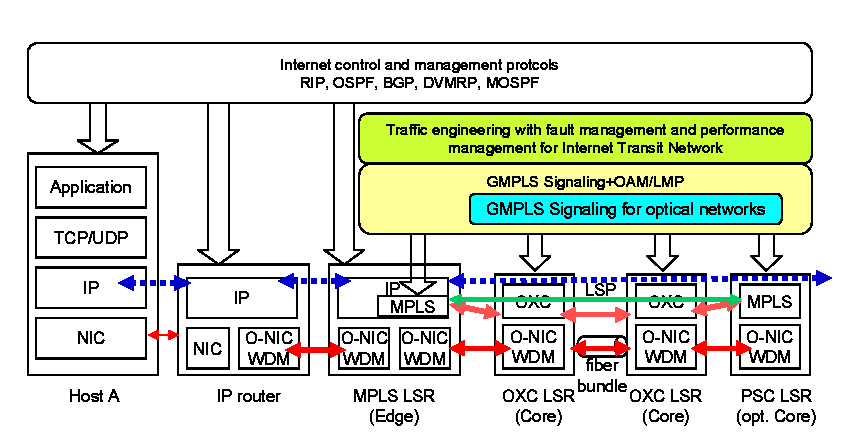
\includegraphics{Figures/NetworkModelNGN} 
\end{center}
\caption{Internet multi-layered traffic engineering model}
\label{NetworkModelNGN}
\end{figure}

Within the context of GMPLS, three basic control plane architectural models have been proposed: the overlay, peer, and the border models. In the peer model, all nodes keep network state information about all links (physical and logical) across all layers of the network. This entails a significant number of control messages to be frequently flooded across network layers to refresh network state information. The overlay model, however, offers total separation between the network switching layers.  The control planes at each of the switching layers operate independently with no exchange of network resource information between adjacent layers. This results in the entire network being managed inefficiently due to the lack of exchanged information. The border model constitutes a compromise between the two previous models where partial network information is exchanged between adjacent layers providing to more efficient and intelligent usage of resources.

Although it is considered that suitable border model architecture can benefit from the advantages of both the overlay and peer models, to our knowledge, there has been a modest effort done to propose efficient provisioning algorithms for this model. As well, within this context, there is little understanding regarding what kind of information would be most helpful in managing routing and signaling decisions in this architecture.

%======================================================================
\section{Motivation}
%======================================================================
Computer networks today have become ubiquitous with increasingly number of services being offered to their end-users. Service Providers (SPs) or network operators are faced with the challenge to support a variety of reliable, secure, and flexible network services and applications to their end-users on a common network infrastructure.
The design configuration, reliability and protection issues of Wavelength Division Multiplexing (WDM) networks have extensively been covered in the literature [GHA00][RIC02] [PHI02][QIN03]. However, most existing networks are integrated in a multiple layer network architecture based on a combination of transport technologies or switching layers where end-to-end connections are likely to span multiple carrier networks. Actually, this multiple layer architecture makes today's core network architecture ineffective. The IP directly over WDM proposition is promising to eliminate unnecessary network layers leading to a reduction in network cost and complexity. However, the challenge remains to control, manage and operate existing transport network effectively using a unified control plane that supports the routing of service requests through a series of regions using dissimilar convergence layers.

A key issue in achieving the above is for the control plane to have knowledge of the multi-layer structure of the network, and how services requested are accommodated. Hence, the coordination, integration and inter-working aspects between the separate network switching layers, on one hand, and the different administrative region-networks, on the other, becomes crucial to facilitate the dynamic provisioning of end-to-end guaranteed services onto a single unified network infrastructure.

When considering optimization of network resources, mathematically, this model implies an optimal solution is sought in a multi-dimensional space by sequentially searching different dimensions-one for each crossed switching layer/domain. Hence, an optimal solution in this case is search-sequence dependant, and not guaranteed a global optimum.

The evolution and maturity of  \gls{MPLS} and Generalized MPLS (GMPLS) has enabled the planning and enabling of advanced networks and services by providers worldwide. GMPLS is a versatile solution addressing current problems at the network level such as scalability, quality of service, traffic engineering, and fast recovery by means of local protection techniques such as Fast Reroute or end-to-end protection schemes [LAN05] [BER05]. GMPLS's unified control plane enables sharing topology and resource information (bandwidth usages, link conditions) across multiple layers. The visibility, however, needs to be carefully controlled in order to meet scalability requirements. One way to achieve this is by aggregating information about resources at lower layers, and presenting the aggregate information to the upper layers. This also eases the integrated design of survivable networks and promises an efficient and cost-effective way to dynamically provisioning multi-grade guaranteed services over a single shared multilayered network, key ingredients of which are bandwidth, latency, service resiliency, and pricing. Active discussions are currently held in IETF working groups [IETFcc], and OIF forums [OIF20] to define metrics and parameters that are required for the routing and signaling in such networks.

Constraint-based path computation is a fundamental building block for traffic engineering in  \gls{MPLS} and GMPLS networks. Specifically, path computation in large, multi-domain, multi-region or multi-layers networks is highly complex and may require special computational 

components and cooperation between the different network domains. A Path Computation Element (PCE) [OKI05] that is present in each node or centralized in each domain is capable of computing optimal and/or diverse TE LSP paths, and providing dynamic inter-layers resource optimization (e.g. optical, and packet layers) of the network's primary and backup capacity. 
In addition, it is imperative to have optimal network resource utilization globally across all network layers to achieve better network efficiency, rather than optimizing resource utilization at each layer independently. This process mandates mechanisms to compute end-to-end paths across layers (inter-layer path computation), and mechanisms for control and management of the virtual network topology (VNT) by setting up and releasing LSPs (or diverse LSPs) in the lower layers.

Approaches to provisioning constrained-based paths are broadly classified into three categories: source routing, distributed hop-by-hop routing, and hierarchical source routing. The hierarchical source routing scheme has been regarded as the most promising scalable approach. However, there is little research on the integration of the hierarchical QoS routing scheme in a GMPLS multilayered network. Additionally, there has been little research investigating mechanisms for supporting QoS/SRLG aggregation schemes suitable in large scale GMPLS networks.
In this context, a multi-grade service offers the benefits of flexibility in service offerings, efficiency in using idle resources, graded pricing to accommodate a wide-spectrum of customers, and the ease of network convergence.

%======================================================================
\section{Objectives}
%======================================================================
The proposed thesis addresses the above raised issues, and presents design constructs and algorithms that suitable for large scale hierarchical layered networks. At present, some of the mathematical analysis and results are at a conjectural stage, the resolutions of which will complete this thesis.

In particular, our objective is to design a multi-layered traffic engineering system that is able to dynamically react to traffic changes while at the same time fulfilling QoS requirements for different classes of service. The main building blocks and operations of the system are:

\begin{itemize}
\item A  \emph{hierarchical aggregation} scheme suitable for the integration in the border model multilayered network architecture. The scheme will be applicable to horizontal as well as vertical layers of the network hierarchy and capable of relaying SRLG and QoS detailed/summarized information for failure-disjoint path calculations.

\item A novel \emph{intelligent path calculation scheme}, within a Path Computation Element (PCE) approach, for the computation of service-constrained optimal and failure diverse LSPs across multiple switching layers and domains. Within this context, two path calculation scheme variants will be considered

\begin{itemize}
\item	scheme that assumes partial/aggregated information about neighboring vertical/horizontal layers. This scheme fits well within a single carrier network managed by a single administrative authority, and

\item a scheme that assumes no/minimal exchange of network state information between layers. 
\end{itemize}
\end{itemize}

In achieving the above, the following is the roadmap sought in the thesis to verify the efficacy of the proposed solutions:

\begin{itemize}
\item Study, design and formulate an analytical mathematical model for multilayer network architecture and apply optimization techniques including Linear Programming and heuristics to achieve network resource utilization optimization.

\item Design dynamic QoS hierarchical routing algorithms suitable for large scale networks, and propose a heuristic for routing QoS/SRLG constrained LSPs

\item Analyze and compare results (e.g. call blocking ratio, crankback frequency, etc.) from simulations run over a hypothetical multi-domain network against optimal solutions achieved using analytical analysis.

\end{itemize}

%======================================================================
\section{Thesis Outline}
%======================================================================
The remainder of this thesis is organized as follows. Chapter 2 describes the hierarchical state of transport networks and the different architectural models that are implemented by network operators today. It also describes interactions between the different switching layers to achieve multi-grade services including multilayered traffic engineering and virtual private networks in the context of GMPLS network architecture. Chapter 3 presents an overview of hierarchical network survivability, and taxonomy of protection and restoration techniques including path diversity across vertical and horizontal layers of the network structure. Chapter 4 presents an overview of network resource aggregation techniques found in the literature and an overview of the related work accomplished in this area, including a novel technique to aggregate for SRLG and QoS resource on links found at different network switching layers, and heuristic algorithm for finding a pair of failure-disjoint working and protection paths. Finally Chapter 5 concludes this report with an identification of work items yet to be finished and a research plan.

\chapter{Survey on Existing Techniques}
\label{chapter.Survey}
\markright {Survey on Existing Techniques}

\section{Introduction}

\section{Review of Path Computation Techniques for Interdomain LSPs}
Puype et al. [PUP03][YAN05] propose Multi-Layer Traffic Engineering (MTE) schemes based on two main strategies: a �reactive� one where MTE actions are triggered only by the detection of network congestion and a �proactive� one that tries to keep the network optimal at all times, triggering a reconfiguration whenever optimizations are possible.
Sabela et al. [SAB03] propose an offline multilayered solution for the global path provisioning in GMPLS multilayered optical networks. They propose a new heuristic and to solve an optimization problem with help of the CPLEX solver optimizing network configuration and traffic routing considering both the optical and the electrical layers.
Iovanna et al. [IOV03] propose a hybrid approach for the routing of IP/MPLS LSPs over a WDM layer which takes advantage of a combined use of off-line and on-line routing strategies to optimize the use of network resources. The proposed heuristic approach is composed of two main phases: (i) an initial paths set-up (performed off-line) by means of a successive shortest-path algorithm (ii) an on-line local search procedure (triggered by network congestion detection) based on the deletion of the lightest loaded lightpath and used for improving the resource utilization to allow the accommodation of incoming LSP requests. Compared to the previous scheme, no details are included here to describe when a link can be considered congested.

\section{Review of Protection and Restoration Techniques}
\subsection{Multi-layer Survivability}
Demeester et al. [DEM99] studied survivability in multi-layer transport networks. They provided guidelines for coordination of recovery actions in WDM, SONET, and ATM layers. Quantitative comparisons were given in terms of recovery time and investment cost. Fumagalli et al. [FUM00] also envisioned the cooperation of the IP and optical layers in providing network resiliency. A heuristic based on simulated annealing was proposed to choose the optimal protection/restoration scheme for each link of an IP-over-optical mesh network. Finally, the practical requirements for multi-layer survivability were examined in the recent RFC [LAI02], in which the use of nested hold-off timers was recommended.

\subsection{Multi-Domain Survivability}
As the network relies more on multiple carriers, issues of survivability in multi-domain/multi-area networks are becoming important in the IP-over-optical network community. Huang in [HUA02] introduced a set of mechanisms for establishing LSPs that span multiple routing areas. Papadimitriou et al. [PAP05] analyzed suitability of using the GMPLS control plane in multi-region networks. Finally, RFC 3386 [LAI02] studied interoperable survivability approaches in a multi-provider environment. Criteria that trigger protection mechanisms at domain boundaries, as well as requirements on the interaction of protection mechanisms on both sides of a boundary, were suggested.

\begin{figure}[t]
\centering
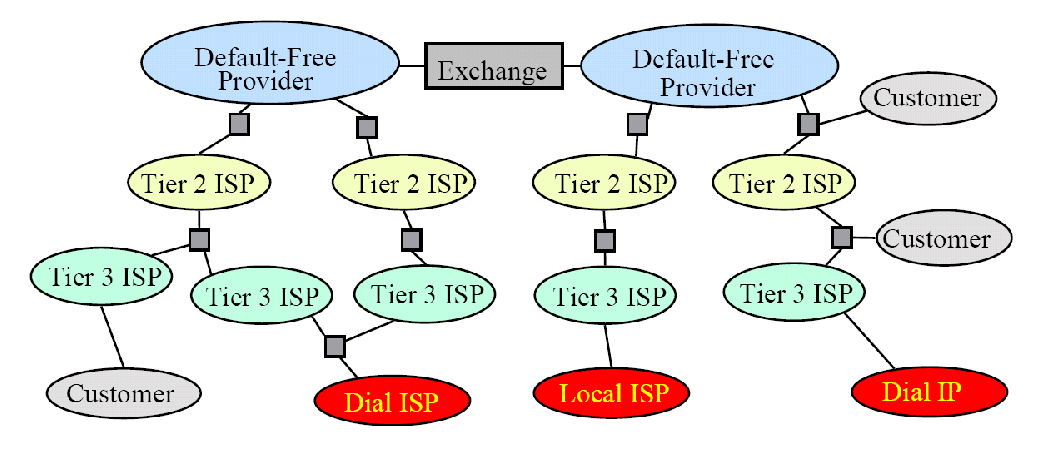
\includegraphics[scale=0.7]{Figures/InternetArchitecture.eps}
\caption{The Internet Architecture}
\label{fig:InternetArchitecture}
\end{figure}

\section{Review of PCE Selection Techniques}
\begin{itemize}
    \item Mesh of separate networks connected at exchange points
	 \item Tier 1 Providers carry full Internet Routing Tables � No defaults
	 \item Tier 2+ Providers carry subset and point to �upstream� default
\end{itemize}

What Is an Intranet?
� A small to global-size collection of interconnected computing resources
available to a closed set of end-users
- could be extended across shared, public Internet or ISP network via tunnels �
VPN
� Applications are distributed (e.g. e-mail) and centralized (e.g. mainframe)
� (Still) based on many protocols � IP, IPX, SNA, Decnet, etc.
- direction towards TCP/IP
� Performance MUST be predictable and Security is ASSUMED
� Internet technologies are now commonplace for corporate networkers
- Web Browser access to corporate resources (including the mainframe which is now just a big server)
- Secure mobile access with performance
- Internet access

\section{Conclusions}

\chapter{Hierarchy of Networks}
\label{cha:HierarchyOfNetworks}
\markright{Hierarchy of Networks}

\section{Introduction to Network Hierarchy}
Hierarchy is a method used in creating scalable and complex systems. It is based on abstraction, at each level, of the most significant of details to the levels further away. Specifically in communication networks, hierarchy is an abstraction of parts of the network's topology, routing or signaling mechanisms. Here, abstraction or aggregation of information is used as a technique to achieve scalability in large networks, or for enforcing administrative, topological, or geographic boundaries. For example, network hierarchy might be used to separate the metropolitan and long-haul regions of a network, to separate the regional and backbone sections of a network, or to interconnect service provider networks.

In our study, we will concentrate on the network hierarchy from two perspectives: 

\begin{enumerate}
\item \emph{Vertical hierarchy}: between two network technology layers. 
\item \emph{Horizontal hierarchy}: between two areas or administrative subdivisions within the same network technology layer.
\end{enumerate}


\subsection{Multilayer Horizontal Network Hierarchy}

\begin{figure}[ht]
 \centering 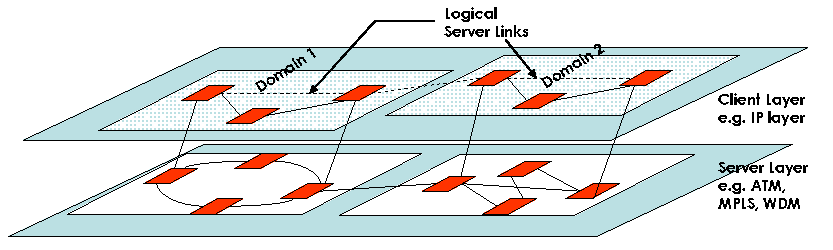
\includegraphics{Figures/HorizLayers} 
\caption{Horizontal hierarchy separation in transport networks}
\label{fig:HorizLayers} 
\end{figure}

Multi-domain horizontal hierarchy is the abstraction that allows a network to scale at certain technology layer, for instance a packet network. Examples of horizontal hierarchy include BGP confederations, separate Autonomous Systems (\gls{AS})s, and multi-OSPF areas.

In the horizontal hierarchy, a large network is partitioned into multiple smaller, non-overlapping sub-networks. The partitioning criteria can be based on topology, network function, administrative policy, or service domain demarcation. Two networks at the same hierarchical level, e.g., two ASes in BGP, may share a peer relation with each other through some loose form of coupling. On the other hand, for routing in large networks using multi-area OSPF, abstraction through the aggregation of routing information is achieved through a hierarchical partitioning of the network.

\subsection{Multilayer Vertical Network Hierarchy}
In multilayer vertical hierarchy, the total network functions are partitioned into a series of functional or technological layers with clear logical, and sometimes physical separation between adjacent layers. Vertical hierarchy, hence, is a generalization that reduces the communication overhead when propagating information across various switching layers of the network; for example, when propagating information between optical and packet switching layers. Figure~\ref{fig:ClientServerLayers} shows interactions between adjacent vertical layers of a network element, as well how vertical network layers form adjacencies between adjacent peering network elements.

\begin{figure}[ht]
 \centering 
 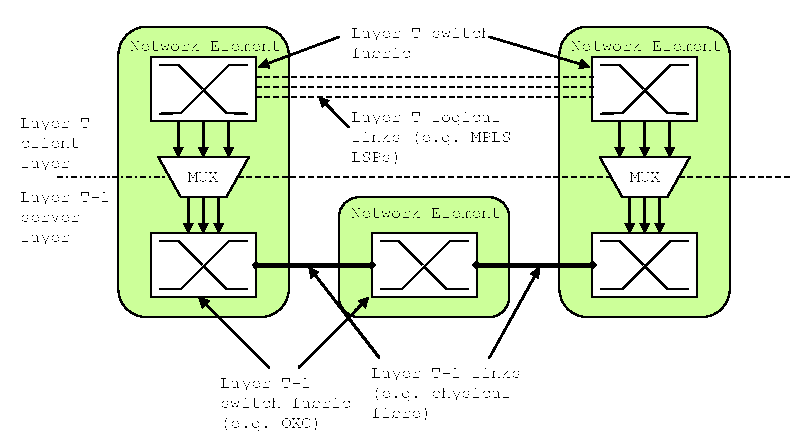
\includegraphics{Figures/ClientServerLayers} 
 \caption{Client-server relationship between vertical layers of network hierarchy.}
\label{fig:ClientServerLayers} 
\end{figure}

\section{GMPLS and Hierarchical Networks}
Several architectural models for the control plane of multilayered networks are in existence today, including the overlay, augmented or border, and the peer models. One of the key differences among these models is how much, and what kind of network information is exchanged between individual layers. \emph{Vertical integration} refers to the collaborative mechanisms within a single control plane instance driving multiple (but at least two) data planes (also referred to as switching layers). \emph{Horizontal integration}, on the other hand, refers to the collaborative mechanisms of control planes extending over several partitions (e.g. IGP areas or autonomous systems) within the scope of at least one data plane instance or veridical switching layer. In this case, the relation between the various horizontal partitions constitutes a peer-to-peer relationship as opposed to a client-server relationship as in the case of vertical integration model {[}KOO04].

\subsection{Overlay Model}
In the overlay network model, the nodes in each layer maintain network information about nodes and links residing in the same layer- such as residual capacity on existing logical links and number of available ports- which makes it more suitable in the case with different management/ownership in each layer. The upper layer only receives a response from the adjacent lower layer on whether or not the requested connection can be set up. There is no specific network information exchanged between individual layers, since the routing in each layer is done separately with each layer's own signaling and control plane.

Hence, in this model, each network layer has to decide whether it will use the existing logical links in its topology or try to create new connections/logical links, and how to route the new request over the existing logical topology without any network information from the lower layer. Each layer's control plane is strictly separate from its adjacent one and runs its own routing and signaling instance protocols,and no information is shared among the two.

\subsection{Peer Model}
In the peer model, the topology and other network information (\eg routing and link state) are shared among all network elements across all the layers by a unified signaling protocol and control plane (\eg single control plane instance for packet and optical layers). Such a model is appropriate when the transport and service networks are operated by a single entity.

In this model, each LSR keeps information about the topology and status of links (\eg bandwidth availability on packet links, and availability of each wavelength at the WDM layer) as well as logical links in the IP/MPLS layer. As often visualized, a network in the peer model can be seen as one graph with both LSRs and OXCs interconnected with physical and logical edges. In this case, an integrated routing can be done with a unified control plane. For example, the integrated routing scheme decides routing over existing logical links, and routing and wavelength assignment (RWA) in the WDM layer at the same time. Note that this is a fundamental difference in the dynamic \gls{LSP} provisioning problem between the peer model and the other two models. In the overlay and augmented models, the RWA in the WDM layer is beyondthe scope of the \gls{LSP} provisioning problem in the IP/MPLS layer.

While in the overlay model global resource usage optimization is not guaranteed - since every layer is optimized in isolation, in the peer model, all layers collaborate in order to achieve some common performance objectives. In this case, a globally optimum solution does not necessarily mean that the individual layers are also optimized. In the peer model, each network node has complete knowledge about the network status (traffic flows, links used, available optical resources, and available capacity in the already established routes), and the entire network can self-adapt dynamically to traffic changes.

\subsection{Border Model}
The border model (also known as the augmented model) provides a compromise between the two extreme cases of peer and overlay models by running separate routing protocols in each layer but still allowing the exchange of partial network information between them- for example, reachability and/or summary of link state information and residual capacity -- depending on a necessary and specific agreement between the two layers.

For example, the IP/MPLS switching layer may utilize a small amount of capacity information passed from the WDM switching layer- for example, the number of lightpaths that the WDM layer can further provide between
every LSR pair in the current state of the WDM network. Hence, a network in the augmented model has to make the same provisioning decision as in the overlay model except that it has more information about the status of the adjacent layers.

\section{Quality of Service}
The notion of \gls{QoS} and network performance are defined in ITU-T Recommendation E.800 (ITU94) as follows:

\begin{quotation}
\emph{{}``The Quality-of-Service is the collective effect of service performances that determine the degree of satisfaction of a user of the service. The Network performance is the ability of a network portion to provide the functions related to communications between users.''} 
\end{quotation}

End-to-end \gls{QoS} ordains that all network layers from top-to-bottom, as well as every network element from end-to-end work collaboratively to provide the desired level of \gls{QoS}. Any \gls{QoS} assurances are only as good as the weakest link in the chain between sender and receiver. End-to-end \gls{QoS} service can be achieved by signaling and reserving the network resources in advance before transferring data.

Often, \gls{QoS} is seen as the need for networks to provide performance bounds on offered services. In other instances, \gls{QoS} is measured in terms of network survivability or availability in the presence of failures. The traditional best-effort Internet was not designed to support a specified, desired, or consistent level of \gls{QoS} to network traffic. Nonetheless, customers now require mission critical services-- such as corporate \gls{VPN}s and radio access networks that demand high levels of network availability and guaranteed levels of service under heavy traffic loads. Service providers now use sophisticated \gls{TE} mechanisms to manage their networks to meet these demands.

\subsection{QoS in Multilayered Networks}
As mentioned, \gls{SLA} levels and \gls{QoS} parameters can be defined on all seven levels of the OSI network model. For example, the Differentiated Services (\gls{Diffserv}) defines mechanisms to provide service differentiation at layer-3 IP packets. At the \gls{MPLS} layer other models, e.g. EXP-inferred \gls{LSP}s (E-\gls{LSP}s) and label inferred \gls{LSP}s (L-\gls{LSP}s), are used to ensure \gls{QoS} for \gls{MPLS} traffic. At switching layer 2, Ethernet's 802.1p and ATM classes of service (CoS) are used to assure \gls{QoS} to traffic traversing at these layers. At layer 1 (WDM layer), \gls{QoS}
is provisioned by introducing schemes to partition wavelengths and classify them into different sets, each being used to service one or more traffic types. This segregation prevents traffic of one type impacting another. \gls{MPLS} preemption based on \gls{LSP} priority is another feature that provides a way to define the relative importance of \gls{LSP}s that compete for the available resources; for example, it allows the preemption of low-priority \gls{LSP}s in favor of higher-priority \gls{LSP}s within a single switching layer. Moreover several service policies can exist for the definition of \gls{LSP} priorities between different layers.

It is imperative, therefore, that \gls{QoS} parameters at all layers of the communication network be considered in the calculation of a potential path for assuring end-to-end \gls{QoS}. A multilayer \gls{QoS} routing system will require performing the following tasks: 2) aggregate \gls{QoS} information to other levels of the network hierarchy, 1) disseminate \gls{QoS} information parameters, and 3) provide the exact hierarchical \gls{QoS} path computation and resource reservation schemes.

\begin{figure}
 \centering 
 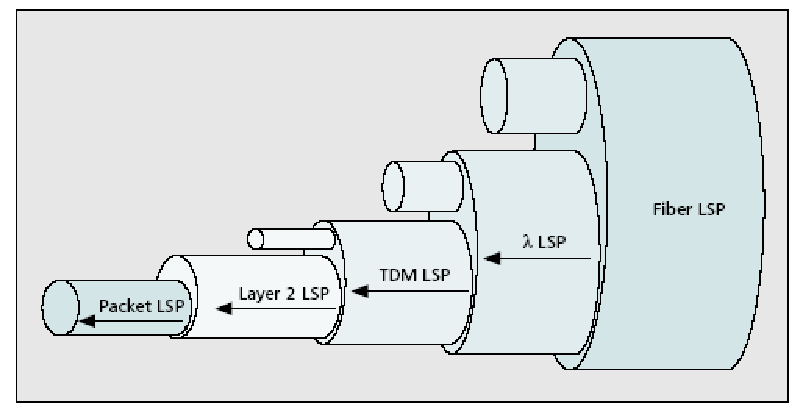
\includegraphics[scale=1]{Figures/HierarchicalLsps}
 \caption{LSP hierarchy in multilayered GMPLS networks}
\label{fig:HierarchicalLsps}
\end{figure}

\subsection{QoS and Traffic Engineering in Multilayered Networks}
The main objective of Traffic Engineering (\gls{TE}) is to improve the efficiency and reliability of networks while optimizing resource utilization and traffic performance. \gls{TE} solutions enable the fulfillment of all these requirements by allowing the network to choose routes for traffic flows while taking into account the amount of traffic load and the network state, or to react to rapid traffic changes or network failures in short time intervals. These solutions can be adopted by using an intelligent unified control plane (such as \gls{GMPLS}), which is able to adequately handle network resources.

Traffic engineering and QoS are strongly related, but to make a difference, QoS controls how the resources are allocated to different users, whereas TE controls where in the network resources are used. Performance optimization of IP networks can be done both at the traffic level and at the resource level. Traffic oriented performance concentrates on the quality of service of traffic streams. Minimization of packet loss and delay, maximization of throughput and execution of service level agreements are the major measures to be improved. The resource oriented performance objectives consist of efficient resource utilization and resource management. Usually bandwidth is the most scarce resource, so a major function is to manage bandwidth allocation.

Both from traffic and resource oriented perspectives the minimization of congestion is crucial. Congestion can be divided into two types, congestion in the case
where resources are insufficient to carry all the traffic, and congestion in the case where resources are divided inefficiently so that a part of network is over-utilized while another part of network has unused bandwidth. The second type of congestion is usually the topic of studies that attempt to minimize it by using techniques provided by traffic engineering by minimizing the maximum TE link utilization. However, TE should still be carried out in such a way that congestion can be managed cost-effectively. 

Performance optimization of networks is actually a control problem. Traffic engineering should provide sufficient control in an adaptive feedback control system. The tasks of a controller consist of modification of traffic management parameters, modification of routing parameters and modifications of resource attributes and constraints [RFC2702].

MPLS-\gls{TE} in packet-based networks provides efficient bandwidth utilization by rerouting traffic via links that are under-utilized. Extensions were defined to enable hierarchical \gls{LSP} establishment-- \eg packet over optical \gls{LSP}s for hierarchical \gls{LSP}s nested inside existing higher-order LSPs. In this case, the preexisting lower-order \gls{LSP} serves as a link along the path of the new \gls{LSP}. Devices form different regions based on their multiplexing capabilities. For example, photonic cross connects define Fiber Switching Capable (\gls{FSC}) devices, Optical Cross Connects (\gls{OXC}s) define the Lambda Switching Capable (\gls{LSC}) devices, L2 switched define the layer-2-switching-capable devices, SONET cross connects define the time division multiplexing (\gls{TDM}) devices, and routers/LSRs define the Packet Switching Capable (\gls{PSC}) nodes. \gls{LSP}s that start and end in a \gls{PSC} region can be combined and nested into an LSP of type \gls{TDM}. \gls{TDM} LSPs in turns can be nested inside an LSC type LSP which can be nested into an FSC type LSP-- as shown in Figure~\ref{fig:HierarchicalLsps}. The new LSPs can be flooded into the routing database to appear as a TE Links.

To perform path computation, a node is able to use conventional links as well as existing LSPs. In optical networks, the traffic coming from upper layers such as IP, ATM, MPLS or SONET/SDH is carried over the logical topology defined by the set of established lightpaths. TE solutions address routing schemes for lightpath set-up, intelligent reconfiguration of the virtual network connectivity (topology), as well as to protection or restoration schemes for lightpath recovery. In a 2-layer IP over \gls{WDM} model, TE can be performed in two main methods, depending on the knowledge of the traffic demand and the level of integration between layers (e.g. overlay, full-peer, or border model).

If traffic demand is known only in terms of an aggregated traffic matrix, the problem of automatically updating the configuration of an optical network to accommodate traffic changes is referred to as Virtual Topology Reconfiguration (VTR). If instead the traffic demand is known in terms of data-level connection requests with sub-wavelength granularity, arriving dynamically from some source node to any destination node, the problem is called Dynamic Traffic Grooming (DTG).

The Traffic Grooming problem has been proven to be NP-hard; thus, heuristics that provide sub-optimal solution are usually applied when connection requests arrive dynamically in realtime. Although many algorithms have been developed to deal with this problem, little attention has been put so far on the \gls{QoS} guarantees for the traffic that simultaneously spanns vertical as well as horizontal layers of
the network hierarchy.

\section{VPNs in Multilayered Networks}
Today, there is increased interest from service providers in offering diverse services and transport solutions for different traffic types over a single common infrastructure. A Virtual Private Network (\gls{VPN}) is usually defined as an overlay network that is built over a public network infrastructure, providing its users with a private and secure network using tunneling, encryption, as well as authentication mechanisms {[}KHA04]. \gls{VPN}s are usually built over various types of public provider networks, such as Frame Relay, ATM or the Internet. \gls{VPN}s are technically classified based on two factors: 1) the underlying technology stack of the backbone transport network that carries the \gls{VPN} application�s traffic (\eg Layer-3 IP/MPLS, Layer-2 SONET/SDH and ATM, or Layer-1 \gls{WDM} core switching networks), or 2) the tunneling endpoint switching layer (\eg Layer-2 Ethernet, Frame Relay or ATM tunnels, or Layer-3 IP tunnels). Figure~\ref{fig:VPNSchemes} shows several \gls{VPN} models that have been proposed to date. For example, a Layer-3 VPN forwards packets based on the \gls{VPN} customer�s IP information, while a Layer-2 \gls{VPN} forwards Layer-2 frames based on information in custaomer's VLANs, MAC addresses, ATM VC Connection Identifiers (VCID), etc. Both of the previous mentioned examples, however, can be carried over a Layer-1, Layer-2, or Layer-3 core based network. Two major flavors of VPNs exist: Provider Edge based (PE-based) and the Customer Edge based (CE-based). Both offer transport services for Layer-2 as well as Layer-3 traffic.

\begin{figure}[ht]
 \centering 
 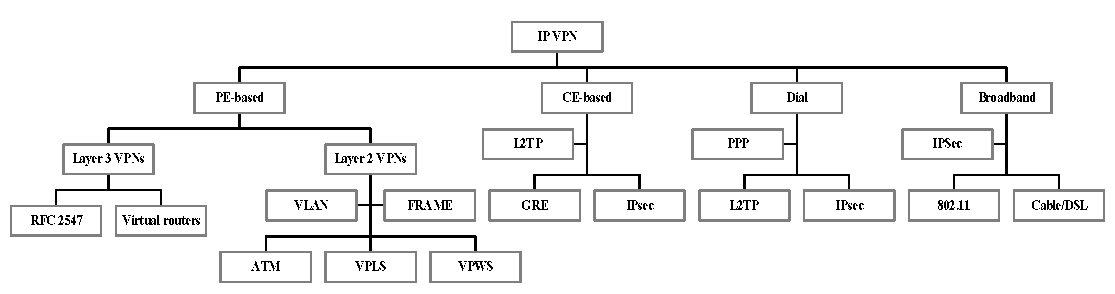
\includegraphics[scale=0.85]{Figures/VPNSchemes}
 \caption{IP VPN protocol implementation schemes.}
\label{fig:VPNSchemes} 
\end{figure}


\subsection{VPN Security}
Security is considered a key aspect in implementing VPNs. To achieve maximum security, customers� encryption and authentication are usually required. Encrypting the customer�s \gls{VPN} traffic prevents other customers in other VPNs from sniffing the data in case of misrouting within the provider�s network. Moreover, authenticating customer \gls{VPN} traffic filters incoming traffic at the Customer Edge or Provider Edge to ensure authenticity of the received traffic. As shown in Figure 1, there are two basic security models that exist within \gls{VPN} implementations: 1) Provider-Edge based security model and 2) the Customer-Edge based security model. In the PE-based model the provider manages and secures communication of traffic crossing its edge boundaries, whereas PE-CE links fall out of its scope of responsibility. In the CE-based \gls{VPN} security model, the connection�s security is covered from end-to-end. The security rules and configuration are done at the customer's side and the provider's edge only provides a transparent media for end-to-end connectivity. Hence, the CE-based security model inherently provides a more stringent and secure implementation of \gls{VPN} than its PE-based counterpart. MPLS and \gls{VLAN}s, by themselves, provide little security for traffic transported over them. In order to enhance security, it is possible to augment them with IP sec tunnels that run from PE-to-PE. This consists of applying IPsec in transport mode to IP tunnels transported over tagged \gls{VLAN}s or MPLS LSPs. The \gls{VLAN} tags or MPLS labels are used ensure privacy and segregate traffic from different VPNs.

Within the Service Provider network, forwarding is based on labels, not on IP addresses carried in the packets. The MPLS switching paths for \gls{VPN} traffic originate and terminate at a PE. They do not begin or terminate in the middle of the Service Provider network. Logical ports on the PEs are associated with VRFs and thus with VPNs at the provisioning time.

MPLS \gls{VPN} privacy is similar to the traditional form of WAN such as Frame Relay and ATM. It provides separation of the traffic between the private customers' networks carried on the Service Provider backbone. MPLS \gls{VPN} establishes network privacy via constrained distribution of routing information and encapsulation of the \gls{VPN} site traffic with a label header in order to traverse an MPLS core. It does not, however, provide firewall security or encryption on the packet, so when \gls{VPN} sites are connected to Extranets or the Internet, additional security measures are necessary to maintain the customer network privacy.

\subsection{VPN Reliability}
Existing transport networks run a variety of network technology layers such as IP, ATM, Gigabit Ethernet, SONET, and \gls{DWDM}. The degree of availability of a connection depends on the proper identification and selection of the protection layer through which the connection traverses. In general, a connection can be protected against failures that occur at the uppermost containing layer as well as layers that fall below. For instance, in a traditional IP multi-layered transport network, a protection layer for a connection can be any of the layers IP, ATM, SONET, down to DWDM. It is possible to apply redundancy or protection techniques at one or more of the transport network layers. However, care should be taken to the tradeoffs between recovery-time and network resource utilization when choosing the appropriate protection  layer. There are mainly two methods for implementing protection on any of these layers: 1) the proactive approach-- typically referred to as protection, and 2) a reactive approach-- also referred to as restoration. In the proactive approach spare capacity is signaled and reserved at connection setup time. In the reactive approach, spare capacity is signaled and reserved after failure occurs. There are several solutions to implement redundancy at each of the layers of a transport network, among them are: the Spanning Tree Protocol (STP), the multi-link trunking, MPLS�s protection and restoration techniques and DWDM ring protection techniques.


\subsection{Classification of VPNs}
\subsubsection{CE-based VPNs}
In a CE-based \gls{VPN}, the CE performs all the \gls{VPN} configuration and provisioning setup. For example, the customer has to engineer provision and maintain a mesh of tunnels or virtual circuits between endpoints of remote sites. The provider only provides a transport for normal IP packets as they travel to and from the CE routers without any knowledge of a customer�s \gls{VPN} routing or addressing scheme.  
Notably, this scheme entails an $O(N^2)$ scalability and attendant complexity where $N$ represents the number of connected intra-VPN sites.

An example of CE-based \gls{VPN} implementation is shown in Figure~\ref{fig:CePeVPNs}. IPsec and Generic Router Encapsulation (GRE) are two methods for implementing the CE-based VPNs.

\begin{figure}[ht]
 \centering
 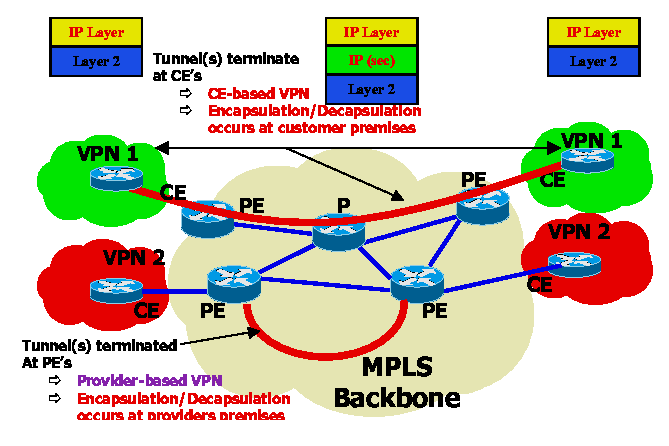
\includegraphics{Figures/CePeVPNs} 
 \caption{Example of CE-based and PE-based VPNs.}
\label{fig:CePeVPNs} 
\end{figure}

CE-based point-to-point VPNs require each router to maintain routing peering with N (CE) devices. This requires the set up of $N\times(N-1)$ connections for full mesh, which will not scale in large networks. With MPLS VPNs, CE only maintains routing peering with one device, which is independent of the total number of sites within the \gls{VPN}.

\subsubsection{PE-based VPNs}
In Provider Edge (PE) based \gls{VPN}, all \gls{VPN} configuration and provisioning are performed on the PE side. The customer edge equipment (CE) connects to the provider PE via a LAN or WAN data link. PE devices hold customer related routes and configurations, while P devices form the backbone devices of the provider�s network. PE-based VPNs solution exists in both Layer-2 and Layer-3. A Layer-3 \gls{VPN} forwards packets based on the \gls{VPN} customer�s packet header IP address. A Layer-2 \gls{VPN}, on the other hand, forwards frames based on information present in the layer 2 frames (e.g. \gls{VLAN}, frames, MAC address, VC Connection Identifiers, etc). Examples of difference PE-based \gls{VPN} implementations are shown in Figure~\ref{fig:CePeVPNs}.

Scalability: only PE routers maintain per-VPN FIBs and run BGP; P routers run IGP only and maintain no VPN state in the core
Customer does not have to maintain virtual backbone, and
the ISP builds/manages tunnels between intra-VPN sites

\subsubsection{Tunnel-based IP VPNs}
In tunnel-based IP-VPNs, a tunnel has two end points where the security service is both negotiated and maintained. Tunneling is a technique used to transfer data for one network over another network. At the start point of the tunnel, the encapsulating protocol adds an outer header over the original packet to form the encapsulated packet. The additional headers provide routing or switching information that enable the encapsulated payload to traverse the intermediate internetwork. At the other end of the tunnel, the outer header is removed and the original packet is recovered. The tunnel itself constitutes the logical path-- otherwise, referred to as a pseudo-wire-- that the encapsulated packets traverse over throughout internetwork.

Tunnels can be applied to various layers in the network protocol stack. It is typically used when transporting or bridging packets belonging to various heterogeneous networks implementing dissimilar protocols for communication. More commonly, tunneling is performed at the data link layer or the network layer.

Tunnels are established across a network for several reasons that include: 

\begin{enumerate}
\item bridging disconnected networks-- for example, to tunnel IPv6 customer packets over an IPv4 \gls{SP} network,
\item providing communication between the home and remote/foreign network in order to reroute traffic destined to the mobile node (\eg in mobile-IP implementation), 
\item providing private and secure communications across a public network,
\item providing connectivity for multiprotocol network layer protocols (\eg System Network Architecture (SNA), IPX, Appletalk, etc.) over a single-protocol backbone, and offering an alternative to source routing.
\end{enumerate}

Tunnels are usually classified based on the type of traffic that they can transport. Example of some Layer-3 IP tunnels include: IP-in-IP (IP/IP), Generalized Routing Encapsulation (GRE), and IPsec tunnels. Layer-2 tunnels include Point-to-Point Tunneling Protocol (PPTP) and Layer 2 Tunneling Protocol (L2TP), and Stacked VLANs (SVLANs). The  Any Transport Over MPLS (AToM) enables MPLS-TE tunnels, however, to
transport Layer-2 as well as Layer-3 traffic. Recently, the IETF has also established a working group named Pseudo Wire Emulation Edge-to-Edge (PWE3) {[}1] which aims at developing standards for the encapsulation
of service-specific PDUs arriving at an ingress logical port and carried across a tunnel.

There are two methods for implementing IP tunnels: 1) the voluntary tunneling and 2) the compulsory tunneling. Voluntary tunneling is client initiated, while compulsory tunneling is initiated at the network access server located at the \gls{ISP}'s point of presence dial-up system. Voluntary tunneling can be used today without requiring any new hardware or negotiating special contracts with an \gls{ISP}.
It is also inherently more scalable than compulsory tunneling, because the tunneling client handles the work of encapsulation and encryption, rather than requiring that this be done on a network device.

\subsection{MPLS-based VPNs}
MPLS offers a scalable IP-VPN solution that delivers value-added services such as security, protection, and support for \gls{QoS} (\eg using \gls{DS-TE}). MPLS also facilitates TE functions by introducing Constraint Shortest Path (\gls{CSPF}) computation features that enable better management of traffic and link utilization in the provider network. Label-Switched Paths (LSPs) can be setup to provide the generic tunneling service to connect segments of a \gls{VPN} over a public provider network, interconnect two non-IP based networks, or define certain treatment (\eg class of service) for packets based on a defined filtering policy. The interior of an MPLS \gls{VPN} network is made up of MPLS-aware P router-devices. PE routers surround the core devices and enable \gls{VPN} functions. P and PE routers act as label switch routers (LSR) that are devices capable of switching packets based on their MPLS-imposed labels.

\subsubsection{Layer-3 MPLS-based VPNs}
The Layer-3 approach to creating MPLS-based VPNs offers a routed solution to the problem. This implementation described in the IETF RFC2547-MPLS/BGP VPNs {[}2] was proposed by the two leader networking solution providers Cisco Systems and Juniper. The approach emphasizes on the use of BGP protocol that already runs at the edges of \gls{ISP} networks and proposes the setup of MPLS LSP-tunnels based on stacked labels that begin and terminate at the PE routers. The inner label identifies the specific \gls{VPN} the packet belongs to, while the outer label determines the path that the packet travels through in the provider network. BGP is used as signaling mechanism for the inner labels while the outer labels� signaling is usually done through LDP or RSVP-TE.

The PE routers exchange routes with the Customer Edge (CE) routers to acquire reachability about the customer's network. These routes are shared with other PE routers carrying the same \gls{VPN}(s) via BGP. Each \gls{VPN} is associated with a \gls{VPN} routing and forwarding instance (VRF). A VRF defines the \gls{VPN} membership of a customer site attached to a PE router. The incoming interface on the PE is used to determine which forwarding table to use when handling a packet because each incoming interface on a PE router is associated with a particular \gls{VPN}. Route Distinguishers (RDs) provide a way of differentiating overlapping routes belonging to different VPNs on the BGP receiver side. When a PE router receives the routes of a given \gls{VPN} site from another PE, it forwards them to the CE router of the connected site belonging to that same \gls{VPN}, so that the CE knows about the networks in the remote site. P routers perform their label switching function without knowledge of the customer's network. Hence, they do not need to share the routes with PE routers.

\subsubsection{Layer-2 MPLS-based VPNs}
The transport of layer-2 traffic, such as Ethernet, Frame Relay or ATM, over an MPLS-enabled transport network has gained recent popularity. Service providers can now use an IP/MPLS core network to offer \gls{VPN}
and Internet access services at the same time. In layer 2 VPNs, the customer data can be forwarded over the MPLS backbone based on information embedded in the layer 2 headers, such as a Frame Relay DLCI, an Ethernet MAC address, or 802.1q \gls{VLAN} tag. Hence, Layer-2 VPNs are inherently Layer-3 protocol transparent, and support the transport of both IP and non-IP traffic. Layer-2 VPNs also eliminate the need
for service providers to participate in a customer�s Layer-3 routing. From a customer�s viewpoint, nothing changes in the network since there are no special requirements on the CE devices and the customer is not exposed to any MPLS technology.

\subsubsection{Layer-2 VLAN-based VPNs}
\gls{VLAN}s represent a standardized Layer-2 mechanism for partitioning a single physical LAN into multiple disjoint logical LANs. \gls{VLAN}s are typically assigned based on the traffic port number, type of the
protocol, the hardware address, or an explicit tag carried within the packet. \gls{VLAN}s provide an efficient mechanism for enhancing performance by reducing the span of a layer 2 broadcast scope. Layer 2 switches isolate traffic across \gls{VLAN} boundaries. Connectivity between distinct \gls{VLAN}s is achieved by routing at layer-3 usually done by a router device. The IEEE 802.1Q standard defines the packet format and required behavior for tagged-based \gls{VLAN}s. The Q tag inserted in the Ethernet frames is limited to 12-bits, or 4096 unique \gls{VLAN} Ids (VIDs). This limits the maximum number of \gls{VLAN}s accommodated within one network.

Stacked VLANs (SVLANs) were introduced to address this shortcoming by adding an additional 4-byte Q-tag header to each tagged packet. SVLANs provide \gls{VLAN} transparency for IEEE 802.1Q tagged or untagged traffic, and can be implemented in a provider network as a PE-based \gls{VPN} solution to provide connectivity to remote \gls{VLAN}s over a publicly share infrastructure. Using this scheme, up to 4096 \gls{VLAN}s can be defined per customer, while the service provider uses up to 4096 SVLANs, increasing the maximum number of accommodated number of \gls{VLAN}s to 4096x4096.

This technology has been widely adapted in Metro Ethernet applications since it provides a very cost effective solution to transport multiple customer \gls{VLAN}s across the service provider's MAN/WAN without interfering with each other. Layer 2 Class of Service (CoS) can further be supported in the core network on per SVLAN basis.

\subsubsection{Layer-1 GMPLS VPNs}
Recently, there has been an increased attention in providing coarse-grained \gls{QoS} using differentiated optical services {[}TOM04]. From the high speed networking perspective, the most promising approach to deliver high bandwidth with the appropriate \gls{QoS} is in an integrated IP over WDM architecture that is facilitated by using the Optical Cross Connect (OXC) and \gls{GMPLS} technologies. The challenge of VPNs in IP/WDM network stems from jointly considering \gls{VPN} provisioning, IP routing, and WDM lightpath configuration. Such a problem can be formulated as a non-linear and non-convex combinatorial optimization problem in which the network construction cost is to be minimized. Problem constraints in this case include \gls{QoS} requirements for \gls{VPN} users and network operators, IP routing
and link capacity assignment, and WDM wavelength configuration constraints.

In IP over WDM network design problem, the two-phase approach is the most common approach. Gouveia et al. {[}GOU03] have proposed a two-phase approach for tackling the MPLS over WDM network design problem. The
first phase solves the core label switching routers placement in MPLS network. The second phase is to determine the physical lightpaths in order to support the logical paths determined in the first phase. However, such an approach sacrifices optimality. Buype et al in {[}PUP03] and {[}PUP05] propose a multi-layer traffic engineering optimization that requires knowledge of the underlying WDM topology. The online
algorithm monitors and reacts to the increase and decrease of bandwidth beyond and below a threshold respectively to set up or tear down links. In our study, we intend to study an integrated approach to jointly
consider the multilayer IP/WDM design problem at the same time, as well take into account VPNs that cross multiple service provider domains.

\begin{figure}
\centering
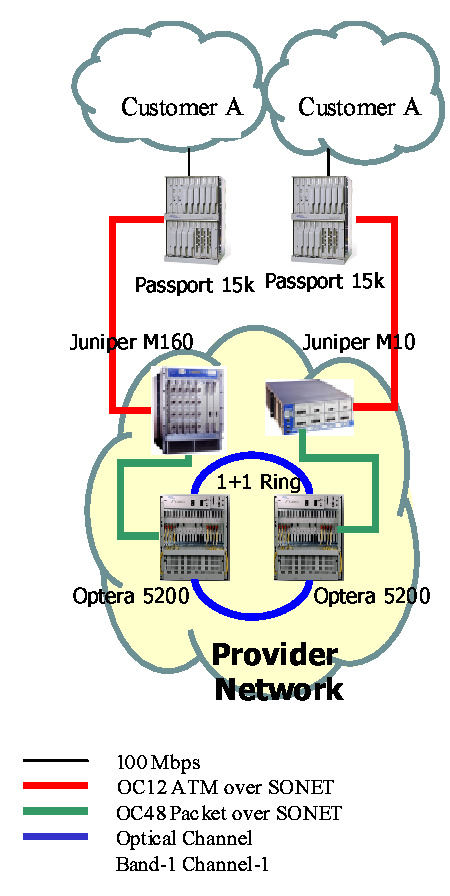
\includegraphics[scale=0.45]{Figures/ProviderNetwork} 
\caption{Layer-3 VPN testbed setup}
\label{fig:ProviderNetwork} 
\end{figure}

\section{Experimental Implementation of Multi-layered VPNs}

In {[}SAA05a] and {[}SAA05c], we published our experiences in the implementation of provider-based VPNs based on different tunneling techniques. Using a metro-based testbed at the Optical Networks Research Lab (ONRL). We described our implementation of several \gls{VPN} tunneling techniques including: 1) Layer-2 virtual circuits using Generic Routing Encapsulation (GRE) {[}HAN94] tunnels, 2) Layer-2 trunks using Ethernet SVLANs {[}IEEE80], 3) Layer-2 tunnels using L2TPv) {[}TOW99], and finally 4) Layer-2 transparent bridging across heterogeneous networks using GRE and L2TPv3 tunnels. Figure~\ref{fig:TBL2VPNs} shows the several configuration setups that were used to implement the mentioned schemes for Layer-2 VPNS.

There are various measurable quantities of interest that can be of indication to the state of the network. For example, available bandwidth, throughput, packet latency, and packet loss, etc. are usually an indication of performance of the network. In this article, we consider the throughput parameter to study different protection schemes that were implemented over the \gls{VPN} solutions discussed earlier.

\begin{figure}
\centering
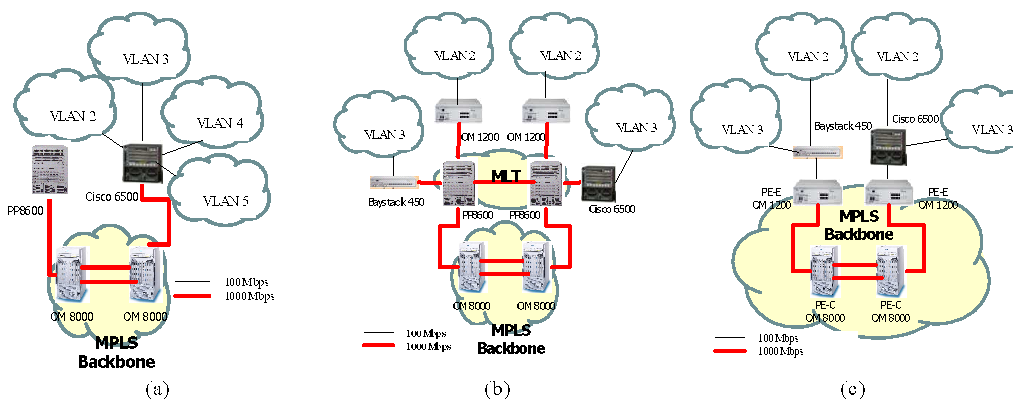
\includegraphics[scale=0.85]{Figures/TBL2VPNs.eps} 
\caption[Layer-2 VPN Testbed setup]
{Layer-2 VPN Testbed setup:
 (a) Switched L2-VPN.
 (b) Transparent L2-VPN.
 (c) VPLS L2-VPN}
\label{fig:TBL2VPNs}
\end{figure}

\subsection{Description of Testbed Hardware}
The testbed that was used to carry out our experiments consisted of multi-vendor equipment from Nortel Networks, Cisco Systems, and Juniper. The Optera Metro 1200 (OM-1200) switch-aggregator was equipped with 10/100 Mbps User to Network Interface (UNI) ports and two Network-to-Network (NNI) Gigabit Ethernet (GigE) interface-cards and were used as CE devices. The Optera Metro 8000 (OM-8000) MPLS switches were equipped with GigE ports and were used in the MPLS backbone. The Passport 8600 (PP-8600) router/switch was equipped with GigE ports and was used as an IP router and as a provider SVLAN-enabled layer 2 switch. The Baystack 425 and Cisco Catalyst 6500 switches were used as an 802.1q-enabled switches that also support layer 2 Class of Service (802.1p) and layer 2 multicast.

Nortel Networks Passport 15K (PP-15K) was used as CE device and was equipped with two OC-12 ATM interfaces, and two FastEthernet ports. Juniper's M-10, and M-160 were used as PE MPLS LSRs, and with OC-48 POS, and OC-12 ATM interfaces. Nortel's OPtera Metro (OM-5200s) DWDM sitches were used as an Optical Add Drop Multiplexer (OADM) for OC-48 POS interfaces. Five Intel-Pentium IV PC-machines were used as traffic sources/sinks in our tests.

Figure 2.5 shows the throughput of TCP flows across the established tunnels described in cases 1 to 4. The throughput was measured while varying the maximum segment size (MSS) of TCP from 350 to 1200 bytes. As expected, as the MSS increased-- \ie\ the payload size increased-- the total number of packets needed to transfer the same amount of data decreased resulting in an increase of the overall throughput of the TCP flow. However, as total packets size exceeded the MTU of the tunnel, we noticed that packets were fragmented before entering the tunnel and defragmented back at the other end point. This resulted in an increase in the overhead and CPU utilization of the routers.

Using a network protocol analyzer, we were able to compute the approximate overhead bytes per packet by sending a 1000-byte UDP datagrams and comparing it with the size of the overall captured packet (after applying tunneling encapsulation in the core of the network). Figure 2.6 shows the overhead per packet as measured when transported over each of the established tunnel in cases mentioned earlier. Results showed that MPLS-based techniques outperformed other IP-based tunneling in terms of overhead in signaling, reliability, scalability and performance. Furthermore, our tests have shown that increasing the size of the transported payload will increase the throughput as long as the packet size does not exceed the MTU size of the established  tunnel. In this case, extra fragmentation and de-fragmentation becomes necessary at the endpoints of the tunnel incurring extra processing power on the routers as well as a decrease in the overall throughput due to the increase in the total overhead.

\begin{figure}
\centering
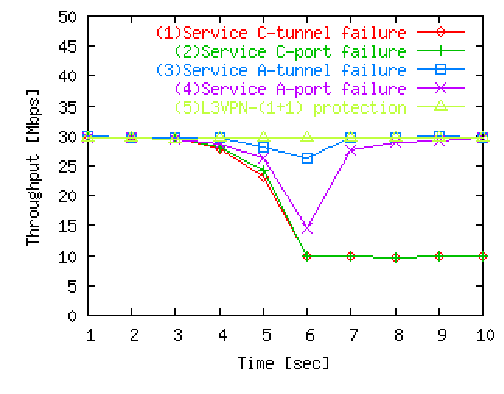
\includegraphics[scale=1]{Figures/ExpResults-01.eps} 
\caption[Throughput of traffic for switched VPN service]%
 {Throughput of traffic for switched VPN service over:
  (1) Service C with tunnel failure,
  (2) Service C with port failure,
  (3) Service A with tunnel failure,
  (4) Service A with port failure, and
  (5) Layer-3 VPN service.}
\label{fig:ExpResults-01}
\end{figure}

\subsection{Experiments Setup}
TODO...


\subsection{Numerical Results}
Figures 6 shows the measured throughput when 30 Mbps of UDP traffic is sent from source-host to a sink-host across the \gls{VPN} implementation scenarios described in previous sections. The abrupt drop in throughput in cases 1 and 2 (at approximately t= 6 secs) coincides with the time that the fault was injected on the primary connection. As expected, recovery from the failure was faster in the case of tunnel failure in one direction as opposed to port failure that brings down the tunnels in both directions of the primary connection. On the other hand, service C (which resembles a best-effort service in our test setup) was allowed only the available bandwidth on the backup tunnels (10 Mbps in this case) -- only after service A had been assigned its full backup capacity. Case 5 shown in Figure 5 represents the throughput of the same UDP traffic transferred over layer-3 \gls{VPN} implementation scenario. In this case, we estimated recovery time of the \gls{VPN} connection between the 2 OM-8000s to be around 27 msec. The downgrade in throughput was barely noticeable.


\section{Evaluation of Protocol Overhead for Tunnel Techniques}
In this experiment, we try to compare the performance characteristics of various tunneling implementations and their impact on the end-to-end data throughput. In each case, an end-to-end virtual connection is established using a tunnel or a series of concatenated tunnels spanning different heterogeneous provider domains each implementing a different tunneling technique. The concatenated tunnels constitute a virtual connection that interconnects remote customer \gls{VLAN} sites.

Generally, there are two types of inter-provider relations that co-exist between different network operators, namely: the peer-to-peer model, and the client-server model. In the client-server model the client domain requests service that the server domain offers. Client network domains receive transport services from their service provider to reach each other. In the peer model, a client network domain is treated as a peer of its service-provider; hence, peer domains not only receive transport services from other participating domains but also contribute new transport services to other domains. For our tests, the Iperf tool was used to generate traffic and measure throughput. Iperf is a tool capable of measuring a number of parameters including bandwidth, throughput, delay jitter, and packet loss.

\subsection{Description of Testbed Hardware}
The testbed that was used to carry out our experiments consisted of equipment from Nortel Networks, Cisco Systems, Juniper and Navtel. The Nortel Optera Metro 8000s (OM-8000s) MPLS switches were equipped with Gigabit Ethernet (GigE) ports, and were used in the ONRL-L2 MPLS domain. The Passport 8600s (PP-8600s) router/switches were equipped with GigE ports and were used in the ONRL-SVLAN domain. The Cisco 3745 routers were equipped with GigE ports and Fast Ethernet (FE) ports, and were used in the IP-based CRC-domain. The Juniper M-10 and M-160 were equipped with GigE ports and OC-12 ATM over SONET interfaces, and were used as Prvider Edge (PE) routers in the ONRL-L3 MPLS based network. Two Intel-based Pentium IV machines equipped with a GigE port were placed in each of the customer�s remote \gls{VLAN}-sites, and were used as traffic sources/sinks in our tests. The Navtel protocol analyzer was used to capture test traffic in order to measure the overall performance and tunnel overhead.

\begin{figure}
\centering
\subfloat[Normalized TCP flow throughput for the implemented tunnel scenario versus maximum segment size.]
{\label{fig:MssThruput}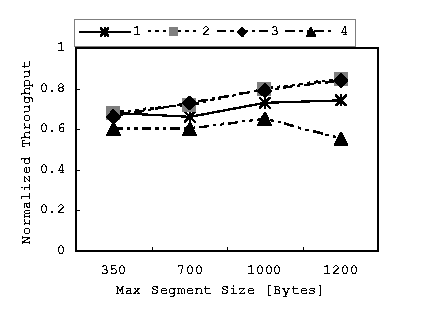
\includegraphics{Figures/MssThruput.eps}}
\quad
\subfloat[Percentage of maximum packet overhead per packet for established tunnels for a 1000-byte packet.]
{\label{fig:TunOverhead}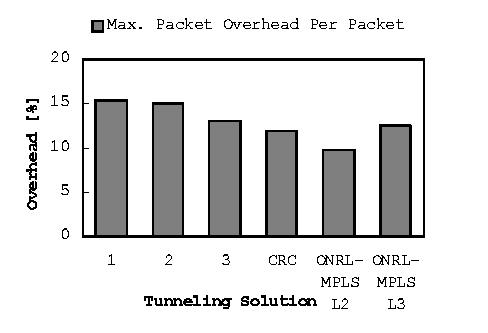
\includegraphics{Figures/TunOverhead.eps}}
\caption{Experimental results}
\label{fig:OverheadResults} 
\end{figure}

\subsection{Experiments Setup}
The purpose of the experiments is to transport \gls{VLAN} traffic over networks running heterogeneous transport protocols. 1) Implementing L2 virtual circuit using GRE: In this setup, the CRC IP-domain, and the ONRL-L2 MPLS domains are employed. The ONR-L2 runs MPLS tunneling service to provide transparent transport for Ethernet VLAN-tagged traffic between the two end PC-clients in the remote \gls{VLAN}s as shown in Fig. 3. In this case, the CRC domain is totally contained inside the ONRL-L2 domain and runs Ethernet over IP-based GRE tunneling service in order to stitch LSPs crossing it from side to side. Ethernet encapsulated MPLS packets arriving at one of the CRC border routers are encapsulated within IP/GRE packets, and then forwarded towards the other border router where it gets decapsulated back to an MPLS over Ethernet datagram and forwarded to the neighboring LSR. Fig. 3 shows the packet encapsulation at each of the mentioned stages.

2)Implementing L2 trunking using S-VLANs: For this experiment, the ONRL-SVLAN and the ONRL-L2 MPLS domains are configured to provide a tunnel connection for the remote PC-clients present in the customer \gls{VLAN}s as shown in Fig. 4. The ONRL-L2 provides transparent transport for Ethernet \gls{VLAN}-tagged traffic over MPLS L2 tunnels. The ONRL-SVLAN domain is totally contained inside ONRL-L2 domain and runs SVLAN tunneling service in order to stitch LSPs crossing its domain boundaries. The Ethernet encapsulated MPLS packets arriving at one of the ONRL-SVLAN border-routers are wrapped within SVLAN packets and forwarded towards the next border router where they are decapsulated back to MPLS over Ethernet frames and forwarded to the neighboring LSR. Fig. 4 shows the Packet encapsulation at each of the mentioned stages. 3) Implementing Ethernet transparent bridging using L2TPv3 tunnels: In this setup, the CRC IP domain and the ONRL-L2 MPLS domains are configured to provide the same service for the PC clients in the customer \gls{VLAN}s as shown in Fig. 3. The CRC domain uses L2TPv3 to establish tunnels that carry VLAN-tagged Ethernet frames encapsulated over MPLS. The Packet encapsulation at each of the mentioned stages is shown in Fig. 3.

4) Implementing Ethernet transparent bridging across heterogeneous network: In this experiment, the CRC, ONRL-L2 and ONRL-L3 are arranged as peer domains that provide transit tunneling-service to end-to-end connections between the PCs in the customer VLAN networks. The ONRL-L2 MPLS and CRC IP domains are configured to provide the same services as described in experiment 1 and 2. The ONRL-L3 domain is configured to provide a layer-3 tunneling service over MPLS as per RFC-2547bis. In order to transfer layer-2 VLAN-tagged frames over layer-3 MPLS tunnels, an IP/GRE tunnel is first established between the ONRL-L3 edge routers. The VLAN-tagged frames are first encapsulated over IP/GRE and then encapsulated over MPLS packets. At the egress edge router, the MPLS and IP/GRE headers are extracted and the VLAN-tagged frame is restored back and forwarded to the customer network as shown in Fig. 5.


\subsection{Numerical Results}
Figure~\ref{fig:MssThruput} shows the throughput of the TCP flow across the established tunnels described in cases 1 to 4. The throughput was measured while varying the maximum segment size MSS) of TCP from 350 to 1200 bytes. As expected, as MSS increased- i.e the payload size increased- the total number of packets needed to transfer the same amount of data decreased resulting in an increase of the overall throughput of the TCP flow. However, as total packets size exceeded the MTU of the tunnel, we noticed that packets were fragmented before entering the tunnel and defragmented back at the other end point. This resulted in an increase in the overhead and CPU utilization of the routers. Figure~\ref{fig:TunOverhead} shows the overhead per packet measured when transported over each of the established tunnel in cases mentioned earlier. In cases 1 and 3, the maximum overhead occurred across the CRC domain. In this case the overhead was composed of an IP, Ethernet VLAN, MPLS, Ethernet, GRE/L2TPv3, IP, and Ethernet header. For case 2, the maximum overhead occurred across the ONRL-SVLAN domain and was composed of an IP, ethernet vlan, mpls, Ethernet, SVLAN header. In case 4, Fig. 7 shows the overhead in each of the three domains: ONRL-L2, CRC and ONRL-L3 individually. In the ONRL-L3 domain, the overhead was composed of an IP, Ethernet VLAN, GRE, IP, MPLS, and Ethernet header.

\section{Conculsions}
In this chapter, we gave an overview of the architectural structure of existing hierarchical transport networks and its different abstraction layers. We highlighted the challenges posed in performing multi-layer traffic engineering and \gls{QoS} routing across vertical and horizontal layers for hierarchical networks. Three basic models for the control plane implementation in \gls{GMPLS} networks were also considered, namely: overlay, full-peer, and border model. The border model is seen as a promising architectural model that addresses the full-peer model�s scalability problems � by only exchanging partial information between switching layers� and offers better utilization than the overlay model by introducing new intelligent PCE schemes at border or edge nodes that can base their path computation based on information from multiple layers. In our work, we will propose to utilize the border model architecture, while revising and extending the information exchanged by \gls{GMPLS} border routers for different domains or switching layers.

This chapter also introduced multilayered VPNs, including traditional layer-3, layer-2, and layer-1 optical VPNs. We presented our findings in some of the works that we have concluded in this area. In Chapter 3, we will consider the survivability issues in multilayered transport networks.

\chapter{Survivability of Hierarchical Networks}
\label{chapter.SurvivabilityOfHierchicalNetworks}
\markright{Survivability of Hierarchical Networks}

\section{Background}
Recent developments in transport networks have resulted in an increasing
concentration of high capacity traffic on fewer network elements.
Hence, the risk of losing large amounts of data becomes imminent and
maintaining a high level of network survivability becomes desirable.
Network survivability relates to the ability of a network to recover
from network element failures. Typically, service providers (or carriers)
provision backup or redundant network resources to protect their services
against network failures. However, they are equally faced with the
objective to efficiently utilize their network resources.

Several factors are considered when designing survivability options
in transport networks. The most important are: resource utilization,
connection request blocking, restoration recovery time, recovery ratio,
recovery granularity, control complexity, tolerance of single or multiple
faults and scalability; the goal being ideally to achieve maximum
survivability with minimum recovery time, while maintaining maximum
resource utilization. It is hard to achieve all these goals simultaneously,
so trade-offs are typically considered when designing a realistic survivable
network. For example, dedicated protection schemes usually offer faster
recovery than restoration schemes; however, they are less resource-efficient.


\section{Protection and Restoration Schemes}

Throughout the literature the terms protection and restoration are
used in slightly different meanings. Protection makes use of pre-assigned
capacity between nodes. This includes the pre-calculation of the protection
path and the preplanning of resources. To provide protection of a
working connection, guaranteed recovery with similar grade of service
and sufficient amount of bandwidth must be set aside in the network.

Depending on the different time-scales in which the spare capacity
is allocated, there are essentially two types of fault management
techniques: protection and restoration. Prior to performing recovery,
the layer closest to the failure is responsible for detecting the
failure. Network nodes communicate with each other to determine where
the failure has occurred and notify other network elements of the
failure. Depending on the different time-scales in which the spare
capacity is allocated, there are essentially two types of fault management
techniques: protection and restoration.

In restoration, signaling is used in real time after the failure occurs
to reroute traffic onto newly computed paths. The LSP is able to compute
the route of the backup LSP according to the automatically updated
routing table after the failures happen. The main disadvantage of
this scheme is its recovery time, mainly due to its dependency on
the slow convergence of IP routing protocols. The advantage of this
scheme is its ability to react to complicated scenarios such as multiple
simultaneous failures.

In protection, however, backup paths are pre-provisioned, and spare
capacity is reserved for them at the time the working path is set
up. Protection techniques can be implemented by several architectures
(for example, 1+1, 1:1, 1:N, and M:N).

Generally, protection is more resource costly, since it requires pre-allocation
of spare capacity for the pre-established backup paths. On the other
hand, restoration may take longer to restore the connection, since
the restoration process happens in real-time. Protection and restoration
have traditionally been addressed using two techniques: end-to-end
path switching and local span/link switching.

Protection and restoration have traditionally been addressed using two techniques: end-to-end path switching and local link switching [XXX].

\begin{figure}
\centering 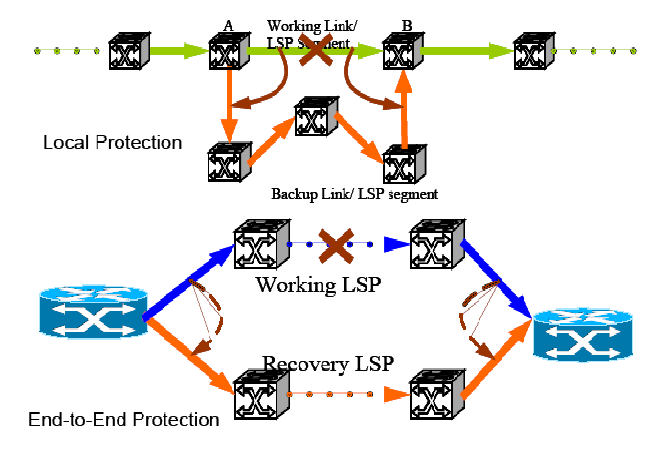
\includegraphics[scale=0.75]{Figures/LocalVsE2EProtection}
\caption{Local versus end-to-end LSP protection}
\label{fig:LocalVsE2EProtection} 
\end{figure}



\subsection{Local versus End-to-End Recovery}
End-to-end recovery refers to the recovery of an entire LSP from its
source (ingress router end-point) to its destination (egress router
end-point). Local/segment recovery refers to the recovery over a portion
of an LSP segment. Figure~\ref{fig:LocalVsE2EProtection} depicts
the difference between local and end-to-end protection.

In an end-to-end path protection scenarios {[}7, 8], a preestablished
backup LSP is set up from ingress label switched router (LSR) to the
egress LSR. In order to guarantee maximum availability, the backup
LSP path is typically routed over a physically disjoint path from
the working LSP. When the ingress LSR is notified of failure on the
working LSP (e.g., reception of a signaling RSVP Path Error due to
the failure of a network component), the ingress LSR immediately starts
switching traffic over to the backup LSP.

In normal situations, the backup LSP does not normally carry any protected
traffic as long any resources along the working LSP have not failed.
For efficiency, and to make best available use of network resources,
it is common practice to allow backup paths to carry traffic (referred
to as low-priority traffic or extra traffic). This low-priority traffic
gets preempted by the high-priority protected traffic when the working
LSP fails.

A similar approach to path protection can be implemented on a link
switching-- also referred to as local link protection. A backup LSP
only spans a link (or a node) to protect this link (or node) {[}FRR].
The backup LSP originates at the protection switch LSR-- also known
as the Point of Local Repair (PLR)-- and terminates in the protection
merge LSR or Merge Point (MP) where the backup LSP is merged with
the working LSP. It is important to note that if a working LSP spans
several links, one backup LSP has to be set up for each protected
link along the working LSP path in order to protect the entire working
LSP.

Path protection reacts to failures more slowly than local protection,
since it takes a significant amount of time to notify the ingress
LSR to switch over to the backup LSP. This leads to more packet loss.
On the other hand, only one backup LSP is needed for one working LSP,
and its global nature allows for less spare resource requirements.

A hybrid scheme named referred to as Fast Reroute was also proposed
FRR. A backup LSP is provided in the opposite direction and concatenated
to a physically disjoint LSP. It combines the best characteristics
of both path and local protection schemes; see {[}9] for more detail.


\subsection{1+1 Protection}

The 1+1 protection scheme refers to the case where one dedicated protection
LSP protects exactly one working LSP or link and protected traffic
is permanently duplicated at the ingress node on both the working
and protection LSPs. Both the primary and backup paths are set up
at the same time, and the required bandwidth is allocated for both.
Upon failure, the destination node can select, independently from
the source node-- \emph{e.g.}, by monitoring the signal quality or
Bit Error Rate (BER)-- the preferred LSP to receive protected traffic
on. Upon failure, the destination can switch (i.e., non-signalled
switchover based on LOS, etc.) from one LSP to another. Hence, $1+1$
protection implicates no signaling delays after failure. Although
such recovery is very fast, it is also inefficient due to the inherent
resource redundancy dictates that extra traffic can be carried over
the protection LSP while the primary or working LSP is active.


\subsection{1:1 and 1:N Protection}

The 1:1 (\emph{aka}, $1-to-1$) protection scheme refers to the case
where one specific backup LSP protects exactly one specific working
LSP/span but the normal traffic is transmitted over only one LSP/span
(working or protecting) at a time. Both working and protection paths
are provisioned simultaneously, but data is only forwarded over the
working path. As a result, protection paths can be used to transmit
low priority pre-emptable traffic during non-failure conditions. As
in 1+1 protection, failure recovery is relatively fast, but efficiency
is somewhat improved.

The 1:N (\emph{aka} $n-to-1$) protection is a extension case of the
1:1 protection. The basic idea of 1:N protection, is that one backup
LSP can protect N working LSPs/spans. When provisioning the working
path, the backup path is negotiated but the allocated bandwidth can
also be used for low-priority traffic (extra-traffic).


\subsection{Shared Mesh Restoration and N:M Path Protection}

Shared path protection builds upon the advantages of 1:N by further
increasing resource efficiency. The backup resources, in this case,
can be shared amongst many LSPs if they fail independently. Since
resources along the protection path are shared, switch nodes along
the protection path are not configured at connection setup. Instead,
upon a failure, source nodes (of failed paths) are notified and generate
signaling messages to configure the switches along the protection
path.

Path-based protection schemes such as 1:1 or n:1 consider the protection
of service traffic between two particular nodes. For path-based schemes,
arrival of a request to establish shared mesh protection service between
two nodes can prompt computation of a pair of disjoint connections
between them. The primary and protection connections would be set
up, meeting the following two necessary requirements.

First, sufficient bandwidth should be available along the route of
the working connection to accommodate the requested load. Second,
either of the following two conditions must hold: either whatever
bandwidth for protection had previously been reserved along the protection
path is already sufficient to guarantee recovery from any single link
or node failure along the new working path, or there must be enough
available bandwidth along the protection path to accommodate the additional
reservation. From the point of view of the network, the degree to
which the additional bandwidth for protection should be shared in
this manner depends on the failure coverage objective for the particular
LSP: whether the objective for the LSP is protection against failure
of any single node, of any single link, or of an SRG.

TODO: FIXME Both shared mesh restoration as well as the N:M path protection
offer sharing for protection resources for multiple working LSPs.
Specifically, in the N:M protection case, N multiple backup LSPs can
potentially protect M working LSP/spans. Backup LSPs .

Shared-mesh restoration, on the other hand, is defined as a particular case of pre-planned LSP re-routing that reduces
the restoration resource requirements by allowing multiple restoration
LSPs (initiated from distinct ingress nodes) to share common resources
(including links and nodes).

%
\begin{figure}
\centering 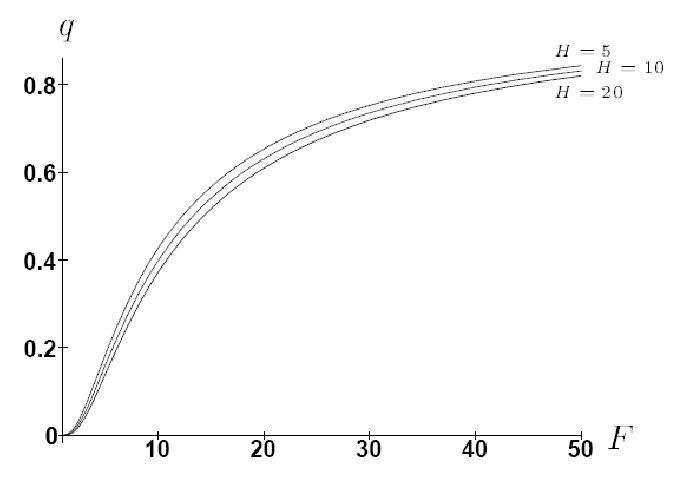
\includegraphics[clip]{Figures/util1} 

\caption{Blocking probability for different path hops \emph{H}}


\label{fig:Utilization} 
\end{figure}



\section{Survivability in Hierarchical Networks}

Transport networks are planned to recover from failures due to a risk
using different mechanisms at different layers. Establishing a primary
path disjoint from the secondary reduces the chances of losing or
dropping traffic for longer time. Indeed, it is imperative to note
that path disjointness at one layer does not necessarily infer physical
path disjointness at all lower layers.

As described earlier, transport networks are structured in vertical
and horizontal structure. This motivates the need to study survivability
of a connection crossing vertical as well as horizontal layers of
the transport network.


\subsection{Survivability across Vertical Layers}

GMPLS networks can be segmented into several areas, such as, wavelength,
waveband, and fiber areas in order to optimize the resilience and
scalability of the networks as shown in Figure 3.1. The achievable
availability of a connection depends highly on the proper identification
and selection of a protection layer. The protection layer is defined
with the following two characteristics: (1) it is one of those layers
below the layer containing the connection; and, (2) the connection
will be protected against resource failures in the protection layer
{[}PIC06].


\subsubsection{Recovery at highest layer}

With recovery at highest layer, the traffic is recovered at the layer
where the traffic is injected. This recovery approach allows the provision
of different survivability classes at a high granularity. On the other
hand, in case of physical failures like cable cuts, a large number
of connections must be recovered individually. This results in a slower
recover performance, as we will attempt to show with simulation results.
With recovery at the highest layer the single layer recovery mechanisms
need not be coordinated, since the mechanisms in the different layers
work independent of each other. At the planning phase of the network
it must however be assured, that client demands of working and protection
network connections are not protected within the server (lower) layer.


\subsubsection{Recovery at lowest layer}

When using recovery at the lowest layer disrupted traffic is restored
at the layer closest to the failure. If a network has to be 100\%
protected against all single link and single node failures, spare
resources in the client layer are only needed for multi-hop client
connections. Due to fault propagation, the client layer detects failures
caused by server layer or physical layer failures. It must be stressed
that the client layer in some cases cannot distinguish whether defect
detection is due to a failure at the client layer itself, or due to
a failure at the server layer. Hence, recovery mechanisms must be
coordinated to prevent a contention between them. Three such interworking
strategies are presented next.


\paragraph{Uncoordinated Recovery.}

In the uncoordinated recovery no interworking mechanism is used to
coordinate the recovery mechanisms. The client layer switches an affected
connection to a backup path as soon as a defect is detected. However,
if the failure occurred in the physical layer, the server layer also
starts the recovery. Due to a time delay between the detection of
failures and the completion of the recovery mechanisms, it may happen
that failures which were already recovered by the lower layer are
again switched to another recovery path in the client layer. This
second switching causes a secondary temporary disruption of already
recovered connections and client layer spare resources will be unnecessarily
occupied. If low priority traffic was carried as extra traffic on
these spare resources, this traffic is unnecessarily pre-empted, causing
additional loss of (low priority) traffic.


\paragraph{Hold-off Time.}

The drawbacks of an uncoordinated recovery prove the need for an interworking
strategy for the coordination of the recovery mechanisms. A simple
and robust interworking strategy is the adoption of a hold-off time
to delay the activation of a higher layer recovery mechanism. The
hold-off time has to be dimensioned large enough so that the lower
layer recovery has enough time to finish the recovery process. If
after the elapse of the hold-off time the upper layer connections
are still affected by the failure, the higher layer recovery will
be activated. The advantage of this solution is its simplicity and
robustness. The obvious drawback is that in some failure scenarios
the higher layer recovery is delayed even if the lower layer recovery
is not able to recover the failure.


\paragraph{Recovery Token.}

To improve the recovery performance in situations where the lower
layer recovery fails, a recovery token delivered to higher layer and
trigger recovery may be employed.


\subsection{Survivability across horizontal layers}

In addition to being vertically layered, optical transport networks
may consist of multiple domains since different carriers or service
providers may want to manage their own parts of the network similar
to the Internet that is formed of great number interconnected Autonomous
Systems (ASes). In this case, a horizontal hierarchical representation
of the network topology can be applied to achieve better scalability.
In this situation, a global connection is likely to cross multiple
domains before it reaches its destination. Connections between regions
or domains can be maintained as abstract (or logical) links. This
process typically includes three main components: an aggregation scheme,
an update policy and a routing algorithm. In Chapter XX, we define
an aggregation scheme that is suitable for calculation of diverse
path at the domain level as well.

We distinguish between inter- and intra- protection techniques for
networks that are separated into several areas. The nodes interconnecting
two or more areas are called border nodes. Intra-area protection implies
that a failure can be restored within the affected areas. This is
done either by local area protection (i.e., by the node adjacent to
the failure) or by the border node on the path to the source. Hence,
local protection is more efficient and faster than end-to-end path
protection across the whole network. Inter-area protection implies
that a connection can be protected against a whole domain failure
and that a connection can be restored by through a path that reroutes
around the failure domain.


\section{Survivability of QoS-sensitive Traffic}

The Internet carries a variety of applications that have varying requirements
for network reliability. For example, some applications, such as email,
do not need the same high reliability as real-time medical or banking
information. Also, it is not cost-efficient to provide equal resilience
to all different type of traffics running over the Internet. Thus,
it would be more realistic to provide differing levels of network
survivability to various traffic types in accordance with the respective
Service Level Agreement (SLA) and try to maximize the network utilization
{[}IWA00].

While the standard routing protocols based on Constraint-based Shortest
Path First (CSPF) algorithms are suitable for establishing new LSPs,
they are too slow to be used for dynamic rerouting of QoS-sensitive
traffic in the presence of node and link failures. In SONET-based
networks bandwidth restoration and protection occurs at the SONET
level. However, where SONET-based restoration is not available, other
protection mechanisms become necessary to ensure that bandwidth guarantees
are still in place upon link or node failure; example of the new emerging
technology that suitable for non-SONET level is Bidirectional Fault
Detection (BFD) Mechanism.


\section{Path Diversity and SRLGs}

One important requirement of survivable network design is the ability
to discover diverse routes for client connections. Multiple connections
are often setup between endpoints for primary and backup paths with
a constraint of being diversely routed. This can include paths that
are link-diverse (i.e. do not share any common link), or node-diverse
(i.e. which do not share any node). This characteristic of path computation
can become complicated when multiple layers (physical and logical)
are considered.

Finding diverse protection paths in a layer in a multilayered network
is a challenging problem. For example, in a hierarchical optical network
an MPLS packet LSP is tunneled inside a lambda-LSP tunneled inside
a fiber-LSP. Multiple fibers are placed into conduits, which are buried
along the right of way (ROW). For economic reasons, service providers
rent ROWs from third parties, such as the railroad companies. As a
result, two diverse fiber links at the OXC layer may be placed into
the same conduit at the conduit layer and are subject to a single
point of failure. Such links cannot be regarded as diverse links when
being used to compute working and protection path pairs. Shared risk
link group (SRLG) was proposed to address this problem {[}XU 03]and
{[}XU 04]. An SRLG is a group of links that are subject to a common
risk. The SRLG concept can be applied to physical as well as logical
resources at all layers of the network

Therefore, finding a pair of diverse paths at the optical layer involves
computing a pair of SRLG-diverse paths. Although the concept of SRLG
was originally proposed to deal with conduit cuts, it can be extended
to include general risks. For example, all the fiber links located
in a geographic area may be assigned the same SRLG considering the
risk of earthquakes. In our study an SRLG risk in this paper represents
a general risk.


\section{Service Availability}

Service availability between two nodes in a network refers to the
ability of the network to perform its primary function (e.g., IP packet
forwarding). This involves physical connectivity, link-layer protocol
connectivity, and network-layer protocol connectivity. Today's ISPs
offer their customers a guarantee of port availability as part of
their SLAs. This simply represents the uptime of a single network
element, i.e., the hardware by which the customer attaches to the
ISP's network. However, this does not, in any way, provide guarantees
about the destinations that a customer can reach at a given point
in time. A key requirement for service availability between two nodes
is the existence of physical connectivity between the nodes (path
availability). A link failure that impacts path availability will
also impact service availability.

It is desirable sometimes to guarantee survivability on per connection
basis, since this provides a means to measure its survivability in
a quantifiable manner. The pre-defined approach to handling LSP protection,
such as letting the high-priority LSPs use optical-layer protection
and the lower-priority LSPs use IP-layer protection, is at times not
sufficient. This is because customer usually demands a more concrete
threshold for guaranteed services. In this case, the connection survivability
guarantee can be specified in terms of minimum connection availability,
defined as the fraction of time the service is available between both
ends of a connection. Several equations describe the basic concepts
that define availability:

\begin{equation}
Availability=1-\dfrac{(Total\ connection\ outagetime)}{(Total\ in\-service\ connection\ time)}
\end{equation}


Availability for devices can be expressed as the following equation
for mean time between failure (MTBF) and mean time to repair (MTTR):

\begin{equation}
Availability=\dfrac{MTBF}{(MTBF+MTTR)}
\end{equation}


The classic availability objective for the public switched telephone
network (PSTN) is to provide 99.99\% availability. Thus, a definition
of service availability in a multilayered network typically considers
the following factors: 

\begin{itemize}
\item network topology, 
\item mapping of IP links onto the underlying physical infrastructure, 
\item inter-dependence of IP network elements, 
\item failure characteristics of links/routers, and 
\item routing protocol convergence time. 
\end{itemize}

\subsection{Hierachical Link Availability}
The availability of a higher layer link (e.g., IP link) depends on
the underlying link layer protection. For example, for a (1+1) protection
scheme at lambda layer, assuming $F_{1}$ the set of fibers that are
crossed by the primary lightpath at the optical layer, and $F_{2}$
the set of fibers crossed along the backup lightpath, the IP link
will fail only when both the primary and the backup lightpaths fail
simultaneously. The availability $A_{l}$ of link $L$ in this case
can be written as:

\begin{equation}
A_{l}(L_{1},L_{2},1+1)=
	\prod_{f\in F_{1}}A_{f}+\prod_{f\in F_{2}}A_{f}-\prod_{f\in F_{1}\cup F_{2}}A_{f}
\label{eqn:1Plus1Availability}
\end{equation}


For a link at a higher layer that is using shared protection (e.g.
1:N) protection, the link will fail if: 

\begin{itemize}
\item both the primary and the backup lightpaths fail, or
\item the backup does not fail but the primary and at least one other lightpath that share the same backup fail at the same time. 
\end{itemize}

Let $F_{b}$ be a set of fibers in other lightpaths that share the same backup lightpath. The availability of a 1:N protected link in this case can be written as:

\begin{equation}
A_{l}(L_{1},L_{2},1:N)=\prod_{f\in F_{1}}A_{f}+\prod_{f\in F_{2}\cup F_{b}}A_{f}-\prod_{f\in F_{1}\cup F_{2}\cup F_{b}}A_{f}
\label{eqn:1For1Availability}
\end{equation}



\subsection{Hierarchical LSP Availability}
Assuming an LSP at a certain network layer $m$ traverses a subset
$L_{u}nprot$ of unprotected links at a lower layer, a subset $L_{1+1}$
of 1+1 protected links at layer $m-1$, and a subset $L_{1:N}$ of
1:N protected links at layer $m-1$, the availability of that LSP
is therefore:

\begin{equation}
A_{LSP}=\prod_{f\in L_{unprot}}A_{l}\bullet\prod_{f\in L_{1+1}}A_{l}\bullet\prod_{f\in L_{1:N}}A_{l}
\label{eqn:LspAvailability}
\end{equation}


The availability of an inter-domain LSP that traverses multiple domains
offering different protection types for each portion of the LSP crossing
the domain:

\begin{equation}
A_{inter-LSP}=\prod_{d=1}^{n}A_{LSP}^{d}-\prod_{d\in d_{1}\cup d_{2}\cdots d_{n}}^{n}A_{LSP}^{d}
\label{eqn:InterLspAvailability}
\end{equation}

\section{Analysis of LSP Blocking Probability}
For the purpose of evaluation of network performance and optimization for different proposed techniques, it is typical to define an objective function. As a natural choice the total \emph{network revenue} can be considered. According to this approach, LSP requests accepted on a certain path $r$ generate revenue at a rate $w_r$, and the total expected network revenue is then:

\begin{equation}
W=\sum_r w_r\lambda_r = \sum_r w_r \nu_r(1 - B_r)
\end{equation}

where $\lambda_r$ is the carried traffic on route $r$, $v_r$ is the traffic offered to path $r$ and $B_r$ is the end-to-end blocking probability for path $r$.

If $w_r$ is proportional to the bandwidth requirement of each LSP request then $W$ signifies the total carried traffic in the network.

Consider a network with $J$ links connected in an arbitrary topology. Denote $C_j$ for the number of circuits in link $j$. At a given instant of time, some of the bandwidth (circuits) on link $j$ will be allocated while the remainder free. Let $m_j$ denote the number of idle circuits on link $j$ , and let $\textbf{m} = \{m_1, \cdots , m_J\}$ denote the network state. The state space is given by $\Lambda = \{0, \cdots, C\} \times \cdots \times \{0, \cdots , C_J\}$.

A path $R$ is a subset of links from ${1,2, \cdots, J}$. Denote $R_j$ for the set of paths that employ link $j$. In order for a LSP call to be set up on path $R$, at least k-units of requested bandwidth must be available at each link $j \in R$. Denote the rate at which LSP calls requests are \emph{set up} path $R$ when the network is in state $m$ by $\lambda_R(m)$. In this case, $\lambda_R(m)$ satisfies:

\begin{equation}
\lambda_R(\textbf{m})= 0 \text{ if } m_j=0 \text{ for some } j \in R.
\end{equation}

Consider the situation where LSP requests arrive to path $R$ at rate $a_R$ and an LSP request is setup on path $R$ if and only if $mj > 0$ for all $j \in R$. Thus,

\begin{equation}
\lambda_R(\textbf{m})=
\begin{cases}
a_R, &\text{if $m_j > 0~\forall j \in R$.} \\
0, &\text{otherwise}
\end{cases}
\end{equation}


\subsection{Unprotected LSP Blocking}
Consider the situation where an ingress LSR attempts to signal an LSP from source $s$ to destination $d$ over a path with $n$ hops. Assuming that an LSP request will be established if at least 1-unit of bandwidth is available on each link, and each link has a capacity of $C$ units of bandwidth.

Let $p$ be the probability that a link $L$ along the path of the LSP is busy (i.e. at least 1 unit of bandwidth is in-use). The expected bandwidth allocation on $L$ can be writtend as $\rho \bullet C$, and $\rho$ in this case signifies the utilization of Link $L$ on this path. An LSP from $s$ to $d$ is blocked if at least one of the links along the path has reached its full capacity (\ie\ fully utilized).

The probability that the LSP request is \emph{blocked} at any link $j$ is:
\begin{equation}
P_b^j = \left( \rho_j \right) ^C
\end{equation}

and the probability the LSP is \emph{admitted} at link $j$:
\begin{equation}
\begin{split}
P_a^j &= 1 - P_b^{j} \\
	  	&= 1 - \left( \rho_{j}\right) ^{C}
\end{split}
\end{equation}

Assuming all links have the same capacity $C$, the probability $P_B^L$ that an LSP request crossing $N$ hops gets blocked can be written as:
\begin{equation}
P_b^L(s,d) = 1-\prod_{n=1}^{N} P_{a}^j
\end{equation}

Rearranging, define the achievable utilization for a given blocking probability as:
\begin{equation}
q=\left[ 1 - (1 - P_b)^{1/N} \right]^{1/C}
\end{equation}	

and for small $\frac{P_b}{N}$, $q$ can be written as: 
\begin{equation}
q \simeq \left( \dfrac{P_b}{N} \right)^{1/C}
\end{equation}

\subsection{Path-protected LSP Blocking}
Considering the case of a 1+1 path-protected tunnel, for the LSP request not to be blocked, both the working and backup paths have to checked and reserved. The probability $P_b(1+1)$ that the request gets blocked can be written as:
\begin{equation}
\begin{split}
P_b(1:1) &= \Pr\{P_b^{work}~or~P_b^{backup}\} \\
		  &= P_b^{work} +  P_b^{backup} - \prod_{\forall j \in R_{work} \cap R_{backup}} P_b^j
\end{split}
\end{equation}

\subsection{Inter-domain LSP Blocking}
Considering the case where an inter-domain LSP crosses $D$ domains from source $s$ to destination $t$. We first consider the case where the blocking probabilities for each sub-LSP portion crossing each domain is determined independently (\ie\ the blockage probability of links belonging to a domain $D_k$ are independent of state of links in another domain $D_l$, we can write:
\begin{equation}
\label{eqn:InterDomainBlocking}
P_b(inter\-domain) = \prod_{i=1}^{D} P_b^{D_i}
\end{equation}

It is possible, however, as we will show in next chapters, in a multi-layered network it is possible that some links be domain-diverse (belonging to different domains) while still share resources at lower layer. In this case, Equation~\ref{eqn:InterDomainBlocking} can be modified as such:

In Figure~, we plot the achievable utilization 


\section{Numerical Results and Analysis}

In this section we present the results of simulation that we ran.
TODO: simulate 1+1, 1:1, 1:N protection schemes. --> Prove that 1+1
has highest availability, then 1:1, then 1:N. Availability= \%of LSPs
that are torn down due to link failure. Simulate multi-area/region
with each area having different protection scheme. --> Prove that
1+1 recovery at lower (bulk) layer makes sense, and that availability=product
of the availabilities being traversed.

\section{Conclusions}

In this chapter we gave an overview of the survivability schemes in
hierarchical transport networks. Survivable network design is a subject
of many past and present studies. In the past, designing a survivable
network involved capacity planning and demand forecast within a single
network layer only. The design of survivable multi-layer networks,
it is a topic that recently attracts both industry and academic interests.
Some of the challenges in provisioning protection and restoration
schemes in hierarchically layered networks lie in identifying link
and/or node failures, and computing failure-disjoint paths. This is
especially significant since a single failure in lower layers can
affect multiple disjoint paths at higher layers.

Another key issue is the careful coordination of recovery actions
at different layers to prevent undesirable function duplication at
multiple layers which results in waste of network resources. Typically
carriers provide escalation in a bottom-up manner due to high reliability
constraint (99.999\% and up) that the optical transport network is
traditionally subject to as opposed to higher layers (e.g. IP/MPLS).
This escalation strategy is based on the old paradigm of independent
layer management. With the GMPLS common control plane, there is a
better opportunity to manage multiple layers in an integrated manner.
As more information is shared among layers, a better way to coordinate
recovery effort among layers is possible. In this thesis, we will
study the interactions between restoration procedures at different
network switching layers, and analyze the needed cross-layer coordination
to minimize spare capacity and protection resources. In Chapter 4,
we will present a novel approach to for hierarchical TE link representation
that facilitates the process of computing multilayer (vertical as
well as horizontal) failure-disjoint paths. 

\chapter{Path Computation Techniques for Inter-domain LSPs}
\label{cha:PathCompTechniques}
\markright {Path Computation Techniques for Inter-domain LSPs}

\section{Introduction}
Path computation in large, multi-domain, multi-region, or multi-layer networks has become more complex and demanding in terms of CPU resources. With the wide deployment of GMPLS and the variety of switching technologies such as packet, TDM and wavelength switching, path computation constraints have increased and have become more stringent than simple bandwidth availability or administrative constraints in packet-switched networks. For example, the path computation of diverse paths in a multilayered network may involve diversity be satisfied with respect to all underlying switching layers (\eg packet, wavelength, fiber, duct, etc, \dots). In addition, as MPLS TE becomes the preferred choice for network operators, and with the rise of Point-to-Multipoint TE (\gls{P2MP-TE}), the computation of remerge-free P2MP paths to a high number of destinations is also becoming a challenge. Therefore, supporting these complex computation problems-- when even heuristic algorithms are computationally intensive-- at every network node becomes an expensive and sometimes infeasible solution.

Inside an AS composed of a single IGP area, all \gls{LSR}s learn the complete topology of the network by means of link-state flooding \gls{IGP} protocol such as ISIS or OSPF. Each \gls{LSR} is able to compute the complete path from head-end to tail-end node for the LSP. However, the topology of an AS is hidden from LSRs that lie outside of that AS, notably for confidentiality purposes. As a consequence, an LSR is not able to compute an end-to-end path for an LSP crossing multiple ASes. Therefore, the computation of such a path has to be distributed among multiple nodes, where each node computes a sub-segment of the path based on its own knowledge of the local domain topology as well as global domain reachability information provided by inter-domain routing protocols (\eg BGP).

In this chapter, we investigate the different approaches to distributively computing such end-to-end paths LSPs that cross multi-area or carrier networks. We present the current state of development of two distributed techniques for the computation of paths respecting QoS requirements together with a centralized technique that we use in subsequent chapters as a reference point to compare with the other techniques. In appendix A, we present our implementation of these techniques in a simulator.

\section{Overview of TE LSP Spans}
In this section, we examine the issues involved in selecting a suitable path for \gls{TE}-LSPs that:
\begin{itemize}
	\item lie within the boundary of a single \gls{IGP} area (also known as intra-area TE LSPs),
	\item traverse inter-area boundaries \ie their path spans multiple \gls{IGP} areas owned by the same carrier  (also known as intra-carrier, inter-area TE LSPs), or
	\item traverse inter-carrier boundaries \ie their path spans multiple carriers domains (also known as inter-AS TE LSPs)
\end{itemize}
Examples of these types of path are shown in Figure~\ref{fig:IntraInterAreaCarrier}.

\begin{figure}[t]
\centering
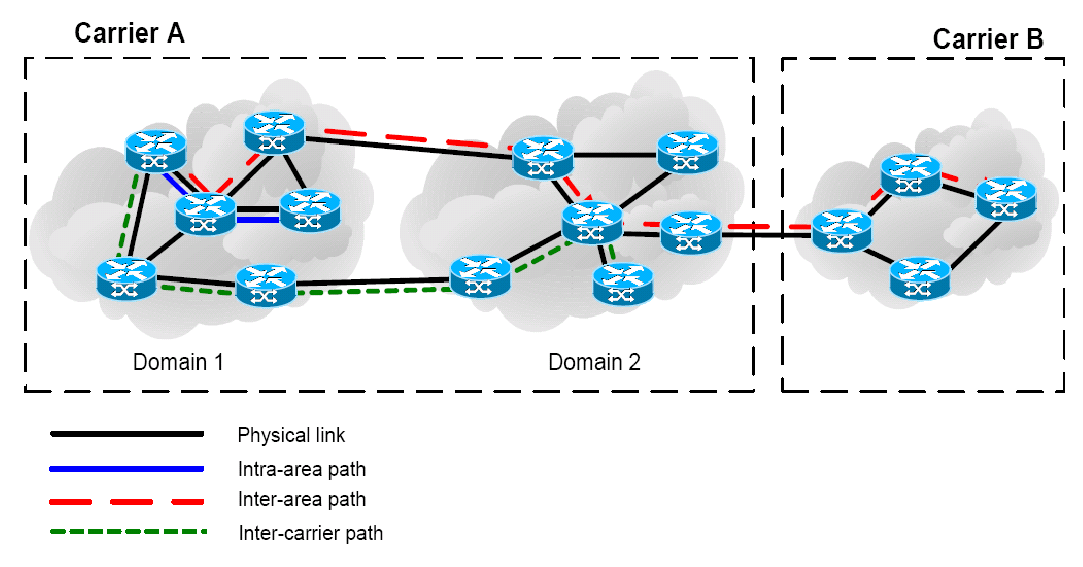
\includegraphics[scale=0.7]{Figures/IntraInterAreaCarrier.eps}
\caption{Intra-area, Inter-area and Inter-carrier paths}
\label{fig:IntraInterAreaCarrier}
\end{figure}

\subsection{Intra-area TE LSPs}
It is relatively straightforward to select a path for an LSP if the ingress and egress points lie within the same IGP area.  The information disseminated by the IGP allows each node to build-up a database of every link in its local area and the appropriate \gls{TE} properties associated with them. If a node receives a request to set up an \gls{LSP} that must meet a certain set of \gls{TE} constraints, then this database can be used to calculate a suitable, complete, explicit least-cost path through the area to the specified egress point of the LSP. If required, the ingress \gls{LSR} can also calculate a diverse backup route (\eg a route that does not use the same link or node) at the same time to provide additional reliability for the LSP.

Typical information flooded by IGPs within a TE-area includes link's: 
\begin{itemize}
	\item maximum bandwidth,
	\item maximum reservable bandwidth: aggregate, per class, and/or per LSP connection
	\item administrative weights (\eg IGP and TE costs),
	\item the Shared Risk Link Group (\gls{SRLG})
	\item delay or latency, and
	\item other characteristics such as resource class attribute color, link availability, \etc
\end{itemize}

As LSPs are established and torn-down, the above \gls{TE} characteristics (such as the available bandwidth) associated with links traversed by the LSPs change dynamically. The IGP, therefore needs to continuously update other LSRs in the same area about the state of their connected links.  To avoid this from happening frequently and causing churn, LSRs could define longer periodic flooding timers. Simultaneously, resource thresholds (\eg available bandwidth) can be set to trigger immediate flooding only when crossed. In this case, if a LSP connection is rejected at any LSR along the LSP path (\eg due to stale resource information at the time of computation of the LSP path), the LSR that blocks the LSP will also immediately trigger flooding of the link state so all other LSRs in the domain can synchronize their TED with recent information.

\subsection{Inter-area TE LSPs}
There are several reasons to divide a single carrier network into multiple areas, including the scalability of the IGP protocol used, administrative convenience, business structure, and compatibility or inter-operability among different vendor equipment.

Unlike the intra-area case, if the LSP must traverse multiple areas, the ingress point of the LSP does not know the details of every link and/or node that could be traversed by the LSP. Since the IGP only runs within a given area, it does not distribute topology information about all the links the LSP might traverse. The information provided by the IGP can no further be used to compute the path up to the Area Border Router (\gls{ABR}) within the area.

However, without this full knowledge a node cannot reliably choose the ``best'' route for an LSP to take-- typically defined as the least cost path that satisfies the constraints associated with the LSP. Instead, the node must try to approximate this function. The goal is to select a path that with high confidence that satisfies the specified constraints without incurring an unacceptable cost in terms of complexity and/or scalability. Generally, there are two ways in which a node can attempt to provide this function.

\subparagraph{Push mechanisms}
\label{par:PushMechanisms}
In these cases, an inter-area routing protocol pushes down a summary of information about all other areas to the nodes in each area. In Chapter~\ref{chap:HierarchyRTAggregation} we discuss in more details how such summary can be formed so nodes obtain a limited or summarized view of the network outside of their own area.

\subparagraph{Pull mechanisms}
\label{par:PullMechanisms}
When using pull mechanisms, nodes do not need to maintain a view of the rest of the network. Instead, when they receive an LSP set up request, they query a remote entity that has a better global view of the network. This entity can further query other sources to collaboratively assist in finding the end-to-end path. On receiving a response to the query, the entity provides the node with a path to the destination that. The \gls{PCE} framework described in Section is one example of this approach. Moreover, In Chapter~\ref{chap:ServiceGuarTE} we propose a novel scheme that falls under this approach that can provide.

Furthermore, there are other complications to setting up protected LSPs spanning different areas. Due to lack of knowledge of all nodes and links along the LSP's working path, it is a challenging tasks for ABR LSR nodes that perform the sub-path computation to find backup LSP paths that protect against node or link failure. In Chapter~\ref{chap:ServiceGuarTE}, we present a mechanism to collect and furnish such information to nodes along the LSP path that would make use of it to compute the such diverse backup paths.

\subsection{Inter-carrier(AS) TE LSPs}
If multiple carriers operate within the network, a single organization will not be responsible for administering the entire network. In order to meet customer requirements, carriers may need to negotiate and provision resources across other carrier's network. The following issues will arise when doing so.

\subparagraph{Issues of Trust}
\label{par:IssuesOfTrust}
When different carriers administer networks, it is critical that a carrier does not disclose sensitive internal information about their topology to other neighboring carriers who may be competitors and can potentially employ the information to gain competitive advantage. For example, carriers may be reluctant to disclose details of the bandwidth available within their network or whether their topology allows them to protect a particular LSP. This makes it much harder to design an efficient path computation algorithm that can calculate paths that span multiple carriers. Also, if a carrier discloses too little information, traffic may sometimes end-up avoiding that carrier network due to the inaccuracy and/or inadequacy of disseminated information which can ultimately  have negative commercial implications.

\subparagraph{Protection issues, standardization and SRLGs}
\label{par:ProtectioIssues}
Setting up a fully protected, end-to-end LSP across multiple carriers is particularly difficult. Nevertheless, ensuring that two LSPs use links in completely different two areas or even different carrier networks does not necessarily guarantee that failure diversity  for the LSP. As different links may use the same physical conduit-- for example different optical fibers may share the same cable and consequently  share the same fate.

To solve this, the Shared Risk Link Groups (SRLGs) can be introduced within the carriers networks. In this case, different links within the carrier network may be grouped together as belonging to a particular SRLG. However, links owned by different carriers can still share the same lower layer infrastructure network(\eg physical conduits). Hence, the concept of SRLG still needs to be extended for the inter-carrier environment to enable nodes across all areas/domains to be able to understand which SRLG is being referred to-- \ie SRLG identifiers need to be standardized across the whole network. This, however, is challenging especially in the inter-carrier environment. A key issue is how to compute paths across multiple areas and/or carrier networks that satisfy the specified constraints.  
In Chapter~\ref{chap:HierarchyRTAggregation} we present a scheme suitable for the inter-area or carrier environment that embeds SRLG information in hierarchical Aggregate Link Resource Tree (ALRT) that is subsequently disseminated to other areas/domains. ABRs, then, can distinguish between links belonging to different SRLGs and compute diverse paths that avoid links of same SRLG.

\section{Inter-domain Path Computation Schemes}
Path computation for end-to-end paths across multiple domains or layers is the next step towards wide-scale deployment of a distributed control plane that supports TE. In this section, we describe three major approaches to path computation for inter-domain LSPs, namely, the IP shortest path, the per-domain path computation, and the PCE-based path computation.
 
\subsection{Inter-domain IP Shortest Paths}
The simplest technique to establish an inter-domain TE LSP is for the LSP path to follow the IP shortest hop-by-hop path. Using this scheme, the RSVP Path signaling messages used to signal the LSP are routed at each hop by performing a IP route lookup for a preferred next-hop (\eg using the IGP routing table for intra-area nodes, or the BGP routing table for destinations outside the AS). Note, this path is usually chosen by Label Distribution Protocol (LDP) LSPs when used between ASs. The drawback of this scheme is that these shortest paths may become overloaded or may not respect the requested QoS constraints.

Figure 4.1 shows the IP forwarding path from node S to node D. This path crosses nodes S-R11-R12-R21-R23-R41-D. More precisely, S determines that R21 is the BGP NH to reach nodes belonging to prefix D/16, based on its forwarding table. From its forwarding table, S also knows that R11 is on the shortest path to R21. Thus, it sends IP packets to R11. The same process takes place at each path on the forwarding path, until the destination is reached.

We note that the end-to-end delay along the IP forwarding path is equal to 115ms. Thus, it could not support a flow requiring a lower delay bound although there might exist other paths (\eg going through S-R11-R14-R31-R32-R41-D, respecting this end-to-end delay constraint. However, this path is not available at node S.

\subsection{Per-domain ERO expansion}
The per-domain path computation scheme defines a technique for establishing inter-domain LSPs where the path is computed during the signaling process on a per-domain basis. It is notably a combination of the inter-domain IP shortest path computation heuristic, and the intra-area path expansion scheme.

The per-domain path computation is applicable when the full ``strict path'' of an inter-domain LSP path is not pre-determined prior to initiating the signaling of the LSP. This usually arises from the lack of TE topology visibility of neighboring TE domains when network state information is not exchanged across domain boundaries. In this case, a set of (loose and strict) hops can be either statically configured at the head-end LSR or dynamically computed at signaling time.


Inside RSVP-TE, it is possible to indicate the path or a portion of the path to be followed by the LSP inside an object called the Explicit Route Object (\gls{ERO}). The ERO expansion technique relies on this object and consists of completing, at the entry ABR of a domain, the path computation up to the next IGP or BGP hop, i.e. last reachable hop toward the destination. This node is usually either the first hop inside the downstream domain or the last hop inside the current domain. The computed path segment is then stored inside the ERO of the RSVP-TE Path message and the message is forwarded along the path inside the ERO. Upon receiving the RSVP Path signaling message, an \gls{ABR} or \gls{ASBR} along the TE LSP path performs a loose hop expansion or partial route computation in its own domain to reach the next loose hop A(S)BR before forwarding the path message downstream.

It is worth noting that such path computation technique does not always guarantee finding a feasible constrained path since it relies on heuristics to choose an appropriate NH among the available NHs announced for the destination (e.g. among the BGP preferred next-hops).  Furthermore, it cannot be efficiently used to compute a set of inter-domain diversely routed TE LSPs. For example, a head-end LSR computes a set of strict path hops up to the first ABR visible in its TE database (TED) topology and then appends the path with loose hops for boundary or domain exit nodes in remote domains. When dynamically computed, the loose hops can be learnt through discovery mechanisms such as IGP, BGP, or policy routing information.

The ERO expansion technique can also make use of the crankback capability of RSVP-TE to stop the establishment of an LSP when a node cannot compute a path toward the destination and attempt different Next Hop (NH) ABR. The ABRs can store the list of NHs that have already been tried for an LSP and lead to an unfeasible path with regard to the constraints. When no NH is found that can complete the path with a segment respecting the constraints, a ``crankback'' is performed by generating an RSVP Path Error message and sending it upstream. The upstream ABR in turn will attempt the expansion of a new segment avoiding the NHs that have already been tried.

As such, the role of crankback is important for the establishment of inter-domain LSPs when only limited information about remotely connected domains is available. If a bad choice is performed by the heuristic at any ABR, a downstream ABR may not be able to complete the computation of the path. Crankbacks enable to cope with such a situation and subsequently try alternative NHs.
 
Figure~\ref{fig:CentralizedPce} illustrates the RSVP-TE ERO expansion technique with path computation that takes place at ABRs. In this example, an LSP with delay constraint of 100 ms has to be established from S to D. Therefore, the source of the LSP $S$ sends out a Path signaling message to $D$. Inside this message (a), the source specifies the tail-end and the constraints of the LSP. When the ABR receives the Path message, it attempts to expand the a path segment respecting the constraints based on its knowledge of the internal topology and the BGP routes for the destination. Then, it forwards the Path message along the computed path segment. 

At the ingress \gls{ASBR} inside AS2, R21, the process described in the previous paragraph is repeated. However, PCE2 is not able to provide a path segment that respects the constraints. The only way, known by PCE2, to reach D is via the NH R41. However, this requires to use link R23-R41. Since this link has a longer delay than the delay constraint for the remaining LSP�s segment, PCE2 cannot return a path segment that respects the constraint to R21. Thus, PCE2 sends back to R21 a PCRep that indicates this situation. Consequently, crankback occurs at R21.

R21 sends a Path Error message upstream. When the Path Error message arrives at S, S sends a new PCReq to PCE1. This request (b) contains in addition to the constraints in PCRep (a), the address of the NH that lead to an infeasible path, R21. PCE1 provides a path segment that ends at NH R23. This NH is also a bad choice. S sends a Path message along the path segment toward R23 and is notified of the failure to continue the establishment of the LSP after crankback occurs at R23 because there is no BGP NH, known by PCE2, reachable with a segment that respects the specified delay constraint.

Upon reception of the Path Error message, S sends PCReq (c) to PCE1 with the constraint to avoid both R21 and R23. PCE1 replies with path segment ending at NH R31 in PCRep (c). A Path message is sent by S along the computed segment. The ingress ASBR, R31, in the downstream AS, AS3, asks its PCE, PCE3, for the computation of a path segment starting at R31 and ending at the entrance inside a downstream AS. PCE3 replies with path segment R31-R32-R41. This path segment is inserted inside the ERO of the Path message and the establishment of the LSP continues until the LSP�s tail-end is reached.

\subsection{The Path Computation Element}
The Path Computation Element (PCE) may be an \gls{LSR}, \gls{ABR}, \gls{ASBR} or any dedicated server that participates in the computation of constrained paths. A PCE is usually assigned to each domain and can compute constrained paths segments within its domain. Paths computed by individual PCE are usually referred to ``local'' path segments. The PCE can also compute an end-to-end path based on the local path segment as well as path segments received from other PCEs. When the head-end and the tail-end of the LSP do not belong to the same domain or, if the LSP has to cross different domains, computation of the path of the LSP is distributed, and multiple PCEs may contribute to the computation of the end-to-end path.

The domain of a PCE may span a single or multiple areas, AS or multiple ASes-- with at least one PCE in each AS. For clarity reasons, we describe the following path computation techniques based on the existence of a single PCE inside each AS. However, they are also applicable (1) when multiple PCEs exist inside ASs with domain covering an AS (\eg AS confederations) as well as (2) when the ASs are divided into more than one IGP area.

The PCE computes path segments respecting given QoS and diversity constraints based on its own TED. The content of the TED depends on the domain of the PCE and contains at the least the topology of the domain and the TE attributes for links belonging to the domain. In addition, it may contain the TE attributes of the links at the border of the domain, for example the inter-AS links.

Moreover, the PCE needs to know about reachability information for destinations outside the domain of the PCE. This information is distributed by the BGP for external prefixes outside the AS. Nodes requesting a path computation from a \gls{PCE} are referred to as Path Computation Clients (\gls{PCC}). Thus, a PCE asking for a computation from another \gls{PCE} acts as a \gls{PCC}. The Path Computation Engine Protocol (\gls{PCEP}) is the communication protocol used between \gls{PCC}s and \gls{PCE}s. A message sent by a \gls{PCC} to a \gls{PCE} requesting a path computation is referred to a PCReq. The response of the PCE to the PCC is a Path computation Reply, PCRep.

An additional mechanism, called PCE discovery, is required in order for the PCCs to learn the list of available PCEs in their domain and in neighboring domains. In Chapter~\ref{chap:EvaluationPCESelectionSchemes} we present an evaluation of different PCE selection schemes as well as present novel heuristic to selecting the preferred PCE among available ones.

\begin{figure}[t]
\centering
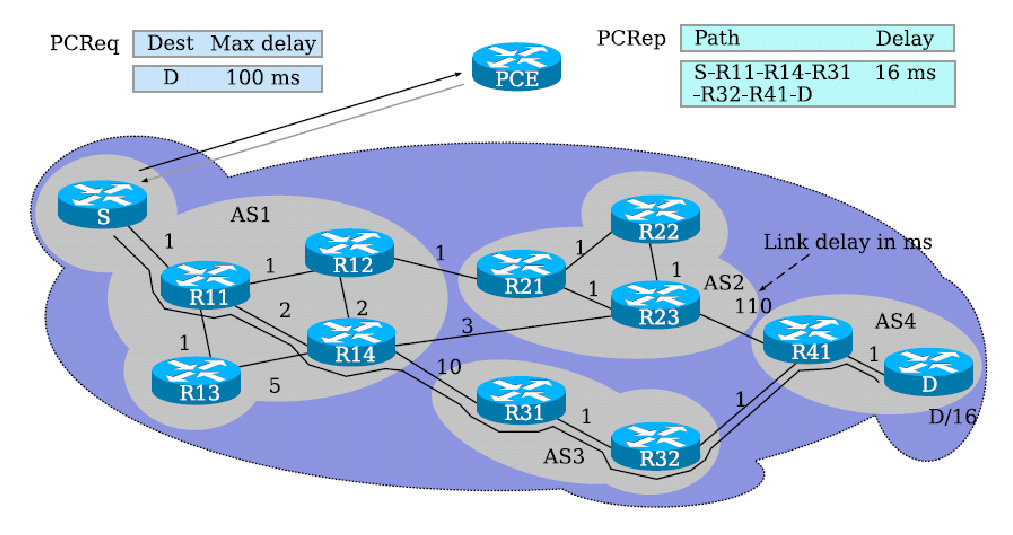
\includegraphics[scale=0.8]{Figures/CentralizedPce.eps}
\caption{Centralize computation with a global PCE}
\label{fig:CentralizedPce}
\end{figure}

\subsubsection{Centralized PCE Path Computation}
Using this technique, the computation is performed by a single entity, that we call ``global PCE''. The domain of the global PCE covers all the domains crossed by an LSP. We assume that the global PCE learns the complete topology by receiving the link state updates from each domain. The global PCE performs as a path computation for each LSP. The algorithm used by the global PCE for path computation is the CSPF algorithm, in this thesis. This CSPF computation by a global PCE provides an indication of the path quality that can be achieved with a centralized computation.

Such a centralized solution could be envisaged when MPLS LSPs are entirely contained within ASes that belong to the same company (\ie intra-carrier case). However, it is not realistic for LSPs that cross ASs from different companies (inter-carrier LSPs) as this requires the ASs to cooperate and reveal their internal topology. As well, this solution also exhibits scalablility issues with the number nodes and links of subscribing ASes. We use this scheme as a benchmark and compare it with our proposed techniques.

In Figure~\ref{fig:CentralizedPce}, we assume that the domain of the PCE covers AS1, AS2, AS3, AS4 as well as their interconnections. When an LSP is required between the head-end $S$ and the tail-end $D$, $S$ sends a PCReq message to the PCE. The constraints required for the LSP are specified in this message. Upon reception of the PCReq, the PCE computes a path that respects the constraints. Then, it sends the path back to the PCC, $S$ in a PCRep message. Here, we see that the path returned by the PCE is the path with shortest delay because the PCE uses the CSPF algorithm.

\subsubsection{Cooperative PCE Path Computation}
A cooperative PCE communicates with other PCEs in order to request or delegate the computation of path segments contained in domains or regions for which it does not possess enough topological information. As mentioned earlier, a cooperative PCE asking for a path computation from another PCE is considered as a PCC.

Using this technique, a PCReq message specifying the constraints for the LSP is relayed from the PCE of one domain to the PCE of downstream domains. Upon reception of the PCReq, the PCEs in downstream domains run a path computation technique to attempt finding path segments starting from the domain ending at the tail-end of the LSP. These segments are sent to the upstream PCE inside a PCRep message.

One such path computation technique, called Backward Recursive PCE-based Computation (\gls{BRPC}) [XXXX] was designed to find the shortest path for a constrained inter-AS LSP makes the assumption that the list of domains to be crossed by the LSP is known prior to the computation. Thus, the computed path is the best path that can be obtained along this inter-domain path. Such assumption is usually applicable in the inter-area case where areas to be crossed by the LSPs are known prior to the computation of the path. This is since an AS is usually divided into a backbone area and stub areas connected to the backbone. The path between two stub areas always goes from the area of the head-end LSR to the backbone area and ends in the area of the tail-end LSR.

However, The above assumption concerning the knowledge of the domains to be crossed by the LSPs holds true if each domain corresponds to an area. However, ASs to be crossed by a constrained inter-AS LSP cannot be known in advance. In Chapter~\ref{chap:ServiceGuarTE} we present a novel scheme that extends the cooperative PCE path computation techniques to finding the list of domains to be crossed by a QoS constrained LSP so suitable PCEs  residing in each can be consulted for path segment calculation.

Figure 4.4 illustrates the computation of inter-AS constrained paths by means of cooperative PCEs. We assume that the list of domains to be crossed by the LSP is not known a priori contrary to [VZB06]. Thus, the PCEs contact a PCE in each downstream domain available from the TED, in order to find the shortest path for the LSP. As a consequence, the optimality of the path found for the LSP depends on the content of TED. Here, we assume that the TED of a PCE is composed of all the BGP routes learned inside the AS6. In general, the TED could be populated
by other means than with BGP. However, a PCE has to be able to determine a set of possible downstream domains from the TED and to contact the PCEs that are discovered inside these domains. The LSP to establish is subject to a maximum delay constraint of 100ms. The head-end of this LSP is router S in AS1. The tail-end of the LSP, node D, belongs to AS4. The longest matching prefix advertised for D is D=16. The central part of the figure shows the physical topology of the ASs and their interconnections. In the top part of the figure, we see the PCEs of each ASs, labels for the messages exchanged between PCEs and the BGP routes known by the PCEs. The content of the messages exchanged between PCEs is shown at the bottom of the figure.

The head-end of the LSP, S sends a PCReq message to the PCE of its AS, PCE1. PCE1 in AS1 has three routes for prefix D=16. We observe from the
AS-path that two of these routes are received from AS2, with two different BGP Next-Hops (NHs) and the other route is received from AS3. Thus, it sends a PCReq message to PCE2 and PCE3, the PCEs inside AS2 and AS3. The PCReq messages contain the address of the tail-end of the LSP and the constraints for the LSP. The delay constraint is not necessary because the output of the computation technique is the shortest delay path. If the delay of the path returned to the LSPs head-end is above the delay constraint, there is no suitable path for the LSP.

PCE2 and PCE3 have one route for prefix D=16. The NH for this route is router R41 in AS4. Therefore, PCE2 and PCE3 both send a PCReq to PCE4.
PCE4 computes a path segment from R41 to D, the tail-end of the LSP. Then, it sends the segment with its delay in PCRep messages (5) and (6) upstream to PCE2 and PCE3, respectively. When PCE2 receives PCRep (5), it has the response to the single PCReq that it sent for the LSP. It has all the requested information. Thus, it is now able to compute path segments from the entrances inside its domain to the destination of the LSP or to determine that is such path segments respecting the requested constraints cannot be provided. For this purpose, the PCE performs a SPF computation on the graph composed of the local topology, the inter-AS links and the segments received from the downstream PCE. The result is two path segments starting at nodes R21 and R23, ending at D. Upon reception of PCRep (6), PCE3 performs the same actions as described for PCE2.

Next, PCE2 sends the resulting segments and their delays inside PCRep (7) to PCE1. In addition, PCE3 sends path segment from R31 to D and the delay of the segment to PCE1, in PCRep (8). Because PCE1 received replies from all the PCEs it sent PCReq messages to, it computes the end-to-end path based on the local topology, the inter-AS links connected to AS1 and the received segments. The resulting path is S-R11-R14-R31-R32-R41-D with delay of 16ms.

This path is sent in PCRep (9) to the head-end of the LSP, S. Finally, S initiates the establishment of the LSP along this path. For this purpose it stores the list of nodes along the computed path inside the ERO. Thus, the RSVP Path message follows the computed path and the LSP is established along this path.

In order to respect the confidentiality requirement of SPs (see section 3.4), PCEs may return path keys [BVF06] inside PCRep messages, instead of returning path segments that reveal sequences of hops inside their domains. A Path Key Sub-object consists of a key that replaces the Confidential Path Segment (CPS) generally contained inside the domain of the PCE and of the identifier of the PCE.
Path Key Sub-objects (PKS) can be stored inside the ERO of the RSVP Path messages. Such sub-object must follow the node responsible for expanding the path key, that is the first node of the confidential path segment. This node sends the path key to the PCE with identifier contained in the PKS for expansion of the path key into a sequence of nodes.

In section A.4 of appendix A, we provide a detailed description of our implementation of this technique. We implemented this technique in parallel to the elaboration of BRPC [VZB06] at the IETF. Thus, our implementation differs from BRPC in matters that were not described at the IETF at the time of our implementation.

Moreover, our implementation solves certain issues that have not yet been considered at the IETF.We show in appendix A that these divergences do not have an impact on the resulting computed paths. However, they induce differences on the information and number of messages exchanged between cooperative PCEs. In the next paragraphs, we give a brief overview of these differences. A more detailed description is provided in section A.4.2 of appendix A. The first difference is that, in our implementation, we do not assume that the list of domains to be crossed by an LSP is known prior to the computation of its paths.

It results that all the PCEs that are downstream of the current PCE on the path to the LSP�s tail-end need to be contacted if the optimal path to the destination has to be found. This difference implies that a PCE may receive multiple requests (PCReqs) for the same LSP. These requests may have crossed a different list of upstream PCEs. Our implementation has to distinguish such PCReqs from PCReqs that are looping. A looping PCReq results in the generation of a Path Computation Error (PCErr) message. The other PCReqs should trigger a PCReq message as reply.

Because PCEs may receive multiple requests for the same LSP, they may benefit from maintaining a cache in order to avoid recomputations and to reduce the exchange of messages with other PCEs. In our implementation, we distinguish two types of PCEs. Stateless PCEs do not maintain a cache with the computed path segments and the responses from the downstream PCEs contacted before, for an LSP. These PCEs need to recompute the local paths segments and to contact all the downstream PCEs each time a PCReq is received. On the contrary, stateful PCEs maintain a cache for each LSP. This cache contains the local paths computed for the LSP and the responses from the downstream PCEs that were contacted for
the previous requests. A stateful PCE does not need to recompute already known local path segments. Moreover, it only sends PCReq messages to the PCEs that did not participate in previous computations for the available NHs.
The second difference between BRPC and our implementation concerns the computation of the local path segments. In BRPC, a PCE computes the segments from its ingress ASBRs to a set of ingress ASBRs inside the downstream domains upon reception of the replies to the PCReqs that it sent. In our implementation, the local path segments are computed on receipt of a PCReq message. We show in section A.4.2 of appendix A that this difference has an impact on the number of messages exchanged during the computation of interdomain paths. In certain cases, BRPC requires fewer messages to be exchanged while in others fewer messages are exchanged with the technique that we implemented.

In section A.4, we describe the algorithm that we use for the computation of the lower and upper bounds on the number of messages that are exchanged in the computation of each LSP with our implementation of cooperative PCEs. The number of messages exchanged for the computation of a particular LSP with our implementation of cooperative PCEs is comprised between these bounds. This number approaches the upper bound if the PCEs are stateless. The number of messages exchanged between cooperative PCEs approaches the lower bound if all PCEs are stateful and maintain the content of their cache during an infinite period of time. The lower bound is also a lower bound on the number of messages exchanged with BRPC. However, we show in A.4.2 that the upper bound on the number of messages with BRPC may be higher than the upper bound computed
for our implementation with algorithm 4.

TSAAD: we need simulations on IP forwarding, ERO expansion and PCE path computation��..

\section{Problem Definition and Formulation}
\subsection{TE Problem Definition}
The problem of concern, hereafter denoted by the TE problem (TP) for short, entails minimizing the overall path cost (\eg typical costs that are considered are IGP or TE cost, or  aggregate transmission delay) over all data flows, each of which is subject to constraints on the link bandwidth capacity. The TP is similar to the restricted-shortest path problem (RSP) [], a NP-complete problem whose goal is to find a shortest path that does not violate a resource constraint. To not violate the constraint, LSPs would tend to be configured along paths that could be longer than the shortest ones, potentially incurring higher costs (\eg higher end-to-end transmission delays, \etc). Thus the minimization of the total cost is pertinent, whereby shorter paths are favored so long as they do not violate the bandwidth constraints. The problem formulation assumes that the data flows and LSPs are one-to-one related. The routing problem is formulated as an integer-programming problem, whose objective function amounts to minimizing the overall cost in all of the links, and whose constraints prevent the violation of the link-bandwidth limits as well as impose the connection-oriented transmission of the MPLS architecture.

In MPLS terminology connections are set-up between an ingress-egress pair of routers. Each connection request arrives at an ingress router
which determines the explicit route for the LSP according to the current topology and to the available capacities at the IP layer. It is assumed that every router runs a link state routing protocol with extensions for link residual bandwidth advertisements.

A connection request $i$ is defined by a triplet $(i_i, e_i, b_i)$, where $i_i$ and $e_i$ specify the ingress and egress routers and $b_i$ indicates the amount of bandwidth required. In the rest of the chapter we will consider only the routing of bandwidth guaranteed connections.

The corresponding LSPs will be routed through the network and, at each instant, one determines the virtual load of a link by summing the bandwidth $b_i$ of the connections passing through the link. The difference between the \textit{link capacity} and the \textit{virtual load} gives the \textit{residual bandwidth}. The \textit{minimum residual bandwidth} over all links of a network is called the \textit{available capacity of the network}. This value identifies the most congested links.


\subsection{Intra-domain TE Problem Formulation}
Consider a single domain IP/MPLS network which consists of LSR nodes and TE links connecting them. Let $\mathcal{N}$ denote the set of LSR nodes and $\mathcal{L}$ the set of TE links of the network. We denote by $l_{ij}$ a link from node $i$ to node $j$. The network topology can be modeled as a directed graph $G=(\mathcal{N},\mathcal{L})$, where $|\mathcal{N}|= n$, and $|\mathcal{L}| = m$. 

Some of the information pertinent to the network topology and links states are characterized by:

\begin{definition}{$\mu_l$}
or $\mu_{ij}$ the capacity of the TE link $l_{ij}$-- \eg the available bandwidth on $l$.
\end{definition}

\begin{definition}{$c_l$}
the cost of transmission when using link $l_{ij}$-- \eg the communication delay on $l_{ij}$.
\end{definition}

\begin{definition}{$a_l$}
the administrative cost of using link $l_{ij}$.
\end{definition}

\begin{definition}{$M_l$}
the maximum allocation multiplier or over-subscription factor of a link $l$.
\end{definition}

We denote the set of LSPs as $\mathcal{K}$. The parameters describing the LSP data flows are:

\begin{definition}{$\mathcal{K}$}
total number of LSPs, where $s_k$ and $d_k$ are the ingress and egress nodes of $LSP_{k}$.
\end{definition}

\begin{definition}{$\lambda_k$}
the bandwidth requested by $LSP_{k}$.
\end{definition}

\begin{definition}{$h_k$}
the maximum allowed number of LSR-hops through the network for a $LSP_{k}$.
\end{definition}

Given the above, the TE constraint-based routing (CBR) problem is charaterized by a set of demands (LSPs)--  described by a set of attributes-- that are to be routed through the network. The objective is to select the optimal placement of LSPs through the network while adhering to the constraints imposed. The unknown variables that need to be determined based on optimizing a certain objective function and satisfying a set of constraints.

The rate of traffic allocated by IE-pair $k$ on link $l$ is denoted by $x_l^k$:

\begin{equation}
\label{eqn:trafficRate}
x^k_l =
\begin{cases}
1, &\text{if $LSP_k \in \mathcal{K}$ is routed over link $l \in \mathcal{L}$} \\
0, &\text{otherwise}
\end{cases}
\end{equation}

The induced load $y_l$ on link $l$ is:
\begin{equation}
\label{eqn:inducedLoad}
y_l = \sum_{k_l \in \mathcal{K}} x^k_l, \quad \mbox{for all $l \in \mathcal{L}$}.
\end{equation}

Load $y_l$ on link $l$ incurs a cost $C_l(y_l)$, which is assumed to be an increasing and convex function of the load $y_l$. The objective in the unconstrained path computation problem is to minimize the total cost by choosing an optimal traffic allocation $x^* = (x^k_l ; k \in \mathcal{K}, l \in \mathcal{L}))$. The problem is formulated as follows:

Resource based optimization would lead to an objective function that minimizes the sum over all links of the product of the cost and the total flow on each link. The cost can be assumed any of the applicable additive defined costs (\eg communication delay, link-availability, \etc).

\begin{equation}
\label{eqn:min1}
Minimize \quad C(x) = \sum_{l \in \mathcal{L}} C_l(y_l)
\end{equation}

Or,

\begin{equation}
\label{eqn:min2}
Minimize \quad z = \sum_{l \in \mathcal{L}} \sum_{k=1}^{\mathcal{K}} c_l \lambda_{k} x^k_l, \qquad \mbox{for all $l \in \mathcal{L}$}.
\end{equation}

The basic set of constraints are:

\begin{equation}
\label{eqn:constraint1}
\sum_{k \in \mathcal{K}} \lambda_k x_l^k \leq \mu_l M_l
\end{equation}

\begin{equation}
\label{eqn:constraint2}
x^k_l \geq 0, \qquad \mbox{for each $l \in \mathcal{L}$ and $k \in \mathcal{K}$}
\end{equation}


\begin{equation}
\label{eqn:constraint3}
\sum_{l \in \mathcal{L}} x_l^k \leq h_k, \qquad \mbox{for all $k \in \mathcal{K}$}
\end{equation}


\begin{equation}
\label{eqn:constraint4}
\sum_{\forall l | i = s_k}  x_{il}^{k} - \sum_{\forall l | i = d_k} x_{il}^k = b_i^k, \qquad \mbox{for all $i \in \mathcal{N}$}
\end{equation}

where:
\[
b_i^k =
\begin{cases}
1, &\text{if $i=s_k$, ingress LSR for $LSP_k$} \\
-1, &\text{if $i = d_k$, egress LSR for $LSP_k$} \\
0, &\text{otherwise}
\end{cases}
\]

Constraint family (2) imposes bounds on the data traffic in each link, whereas (3) . Variable $x_k^l$ takes on value 1 if, and only if, the virtual path of the k-th $LSP_k$ uses link $l$ between $(i, j)$.

From the above set of equations, Constraint~\ref{eqn:constraint1} imposes bounds on the data traffic on each link. Constraint~\ref{eqn:constraint2} guarantees that the nodes selected for each $LSP_k$ form a simple path from its source $s_k$ to its destination $d_k$. Constraint~\ref{eqn:constraint3} imposes a bound on the number of hops for an acceptable path for $LSP_k$. Constraint~\ref{eqn:constraint4} is the flow conservation constraint that states that traffic for each IE-pair incoming to a node has to be equal to the outgoing traffic from that node.

\subsection{Inter-domain TE Problem Formulation}

In the proposed scheme, flows on the inter-AS links are used as constraints for the low-level intra-domain TE problem. For this reason, we assume that the domain being considered, $D_i$, consists of its set of $\mathcal{N}$ nodes and set of intra-domain links $\mathcal{L}$. The topology of Domain $D_I$ can be modelled as directed graph $G_I(\mathcal{N},\mathcal{L})$. Further more, we assume each domain $D_I$ knows the following:

\begin{itemize}
    \item the intra-domain traffic rate load, $x_{ij}$
	 \item the outgoing inter-domain requirements, $x_{iJ}$, where $I \neq J$
	 \item the total incoming traffic destined to an egress node in domain $I$, $r_{iI}$
	 \item the number of LSPs, $x_gJ$, in all gateway links $g$ entering domain $I$ and destined to domain $J$.
			 Denote by $g \rightarrow i$ and $g \leftarrow i$ inter-domain links $g$ \textit{in} and \textit{out} of gateway node i, respectively.
\end{itemize}

The intra-domain TE problem can be formulated as shown in section. The total flow $T_{iJ}$ that a node $i$ in $I$ sends to domain $J$ (including both locally and externally generated traffic) appears like local traffic generated in $i$ is compuated as:

\section{Conclusions}
As we have seen, selecting a path for an LSP that satisfies the LSP constraints is particularly difficult when the LSP must span multiple areas. Different standards bodies are developing different strategies to tackle these issues�the IETF is actively working on drafts ([1], [2], [3], [6]) that show how existing technologies can be leveraged to provide a solution relevant to many packet switched networks. However, the OIF and ITU are currently developing a different DDRP-based approach for optical networks ([4],[5],[7]). This difference is motivated by the significant differences in the requirements of optical carriers in comparison with say, incumbent carriers owning IP networks. Given this, some of these solutions are likely to co-exist in the future. 

Within each of the rough positions assumed by the IETF or OIF and ITU, there are many solutions being discussed. Each solution has its own drawbacks; for example some solutions may not scale well but implementing other more scalable approaches is a significantly more complex issue. However, carriers will not decide which solution to implement on the technical issues we have discussed alone. They will carefully weigh up the investment needed to implement each solution against the savings it could provide to the running costs of their network. It is these factors together that will determine which solutions are accepted by the industry and deployed in tomorrow�s networks.

\chapter{Link Resource Tree Aggregation for Hierarchical Networks}
\label{chap:HierarchyRTAggregation}
\markright{Link Resource Tree Aggregation for Hierarchical Networks}

%======================================================================
\section{Introduction}
%======================================================================
As described in Chapter~\ref{cha:HierarchyOfNetworks}, transport networks consist of hierarchies of network switching layers as well as physically or logically divided domains. To achieve scalability in routing and network state advertisements, domains and switching layers advertise summary, or aggregated views of their internal structure to their peer and client layers. In other cases, topology aggregation is also needed for security reasons to hide the details of the underlying domain from others. In these cases, the aggregation scheme should not misrepresent information about the domains or layer's internal structure.

While Topology Aggregation (TA) is needed to ensure the scalability of the path selection schemes, the reliance on aggregate information to determine an appropriate path for a LSP connection request may sometimes result in infeasible paths being used-- ultimately leading to failing the call admission test at some intermediate intra-domain node. This type of a blockage (due to a discrepancy between actual and advertised information, or due to changes that might have occurred since the last advertisement) causes the LSP connection request to retrace its steps from the point of blockage back to its original entry point into the domain (\eg ABR node)-- a process described in previous chapter as a crankback. Once the request has returned to the point where it first entered the domain or layer, a new path through the domain can be computed; if such a path is found the LSP connection is established, otherwise the request cranks back further upwards towards its origin as shown in Figure~\ref{fig:crankback}. Crank-backs continue until either the network decides that no new path can be found, or the signaling protocol timers expire. Ultimately, the target in general when designing efficient resource and topology aggregation schemes is to have lower such frequency of crankbacks at signaling time which inherently indicates faster setup times for connections and less control traffic load.

\begin{figure}[t]
\centering
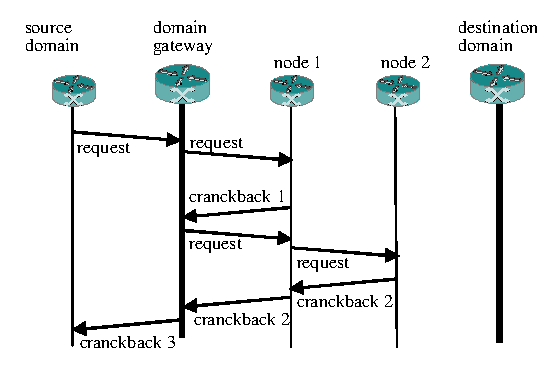
\includegraphics{Figures/crankback.eps}
\caption{Crankbacks with inter-domain signaling}
\label{fig:crankback}
\end{figure}

\section{Hierarchical Path Computation}
State-dependent QoS-enabled path computation schemes necessitate the provisioning of scalable routing solutions that take into account the QoS requirements of prospective LSP connections as well as the available network resources. Examples of such protocols are the Private Network-to-Network Interface (PNNI) and the QoS-enhanced OSPF protocol, both of which are link-state and inherently hierarchical.

In fact, no node in a real network holds the exact state of the complete network in real time due to inherent latencies in distributing the advertised link state parameters. Consequently, the chosen path at the source node may sometimes not guarantee the requested QoS, and each node along the signaled path has to perform its own call admission and that may end-up blocking the call. The goal of aggregation is to achieve a simplified representation of both topology and QoS advertisements.

Using a hierarchical path computation a path is computed based on a mixture of detailed and aggregated state information. A signaling or call-processing entity in each domain will compute intra-domain path or paths between border routers using detailed information about the domain's internal topology and advertises logical link state attributes to its neighboring domains-- see Figure~\ref{fig:TwoLevelHrchy}. Based on the aggregate advertisements between domains, the source-domain call processing entity or border node calculates a feasible inter-domain ``loose path'' for the connection that satisfies the end-to-end QoS requirement. As such, a hierarchical QoS network has to use a QoS aggregation scheme within each of its logical and corresponding physical layers.

\subsection{Topology and Link State Aggregation Procedure}
\label{TopologyLinkStateAggregation}
The extent of aggregation of information and what to aggregate play an important role in determining feasible paths and improving the chances of establishing an LSP request. Yet typically, very little information is conveyed to non-local lower level areas of the hierarchy, \eg in the previous example only prefix reachability information was provided by the BGP protocol. However, for some networks, this could cause significant problems when attempting to set up LSPs that guarantee bandwidth for traffic routed across multiple areas.

Alternatively, carriers can attempt to push a summary containing more information about their network link state to intra-level nodes. There is an important trade-off with doing that however-- \ie increasing the information included in the link state summary, will also increase the amount of information that needs to be stored, maintained, processed, and considered by intra-domain nodes in their path computation algorithms.

At one extreme, an aggregation scheme must not represent any information about a domain's internal structure. In this case, all possible aggregated representations that could be generated will have to include the costs of all possible transits through the domain. Such a representation may be viewed as a complete weighted graph whose vertices are the border nodes of the domain whose edges represent the costs of the corresponding transits. Unfortunately, the size of such a representation grows quadratically in the number of nodes, which implicates scalability problems.

The performance benefits of having higher-fidelity aggregation scheme need to be balanced against real-world burdens imposed by the use of larger representations. Such burdens include having grater space requirements for the topology database within each domain, increase background traffic between domains due to topology updates, and longer computation times for determining the least-cost paths.

The concept of levels is used to help aggregate properties of a particular area. One example of such aggregation would be to represent the Internet as a \emph{level-1} graph with vertices representing abstract nodes and edges representing the inter-domain links-- we refer to this as the simple-node representation. Another aggregation scheme would be to abstract the domain by its ABR that are connected by abstract links-- we refer to this as the complex-node representation. This can be viewed as a complete weighted graph whose vertices are the border nodes of the domain and whose edges represent the costs of the corresponding transits as shown in Figure~\ref{fig:TwoLevelHrchy}.

\begin{figure}[t]
\centering
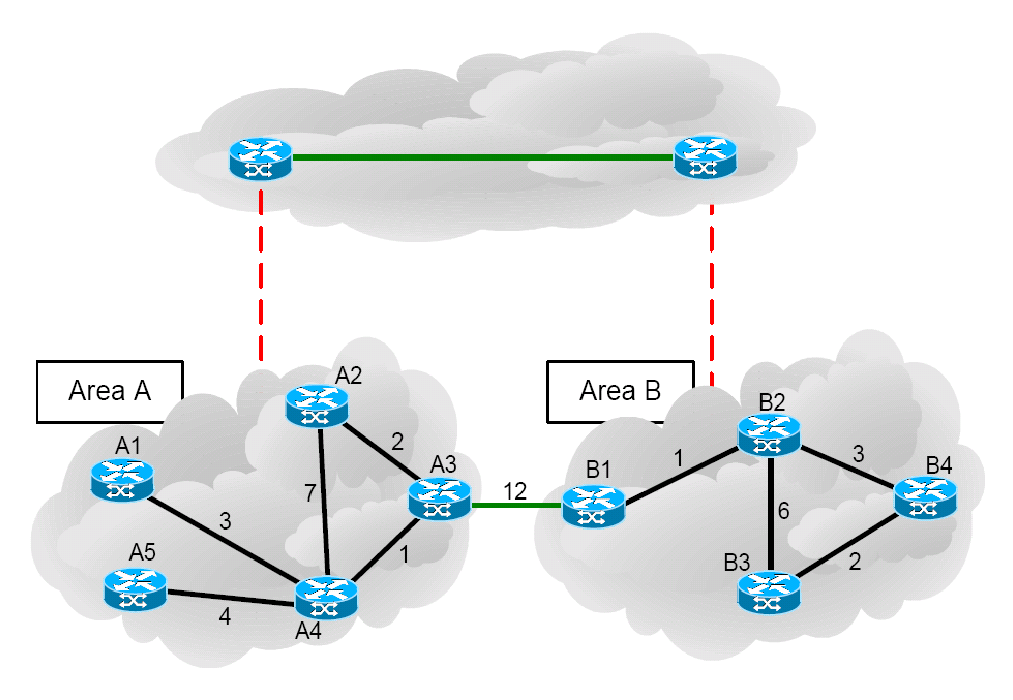
\includegraphics[scale=0.75]{Figures/TwoLevelHrchy.eps}
\caption{Path computation in two level hierarchy networks}
\label{fig:TwoLevelHrchy}
\end{figure}

For example, consider the example of a 2-level hierarchical network in Figure~\ref{fig:TwoLevelHrchy}. In this example, the physical nodes and links are at the lowest level of the hierarchy. The higher level consists of abstract nodes and links that are summarization of the lower level topology.

Every node in each area discovers Link State information about the links and nodes inside that area. These links are physical links, and so they should be viewed as being part of the lowest level. At the higher level, each area is represented by an abstract node. If there is at least one physical link between two areas, then the corresponding abstract nodes have an abstract link between them. The set of abstract nodes at the higher level form a virtual area, and distribute information about each of the an abstract links amongst themselves.

Each abstract node ``feeds down'' summarized information about these abstract links to the lower level nodes in the area it represents. From the perspective of the lower level nodes, there is now a link between node A3 and area B.

It is important to note that the above aggregation scheme equally applies to horizontally adjacent domains at the same layer (\eg IP packet neighboring domains), as well as between vertically adjacent domains (\eg IP and optical layer domains). In the latter case, the border model scheme discussed in Chapter~\ref{cha:HierarchyOfNetworks}, can be used to flood logical link representations (also referred to as forwarding adjacencies) to higher layers (\eg packet layer). Consequently, these FA links can be used in the path computation for requests that are originate at packet layer.

\begin{figure}[t]
\centering
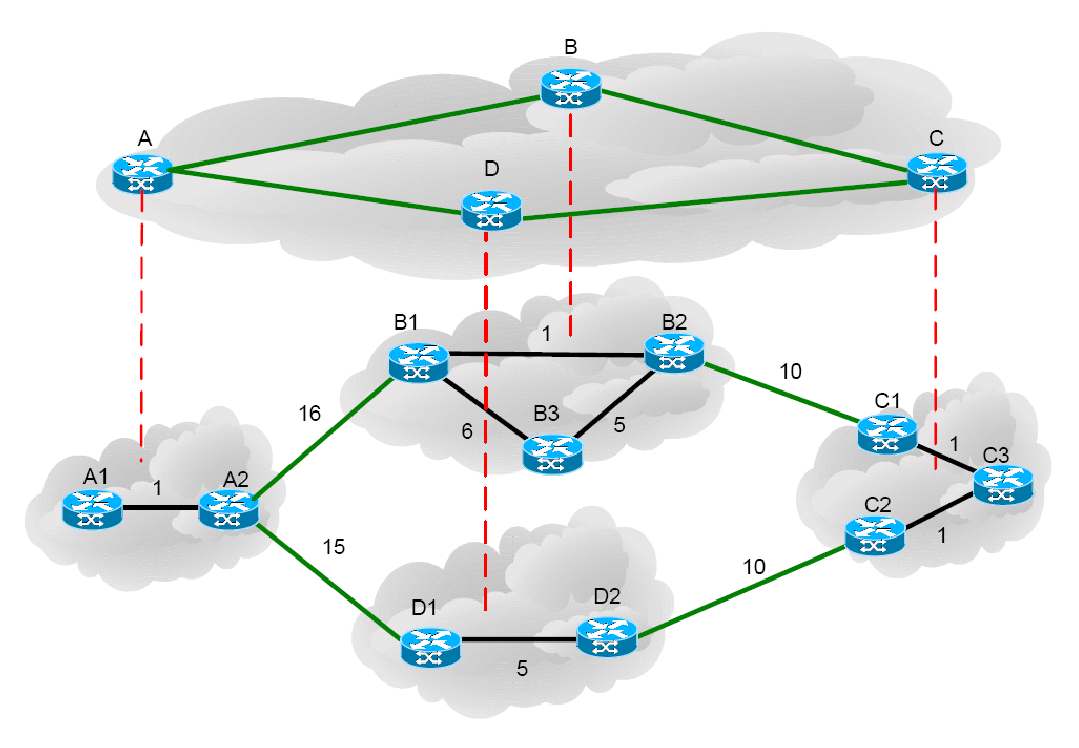
\includegraphics[scale=0.75]{Figures/TEVirtual.eps}
\caption{TE path computation with abstract links}
\label{fig:TEVirtual}
\end{figure}

\subsection{Simple and Complex Node Domain Abstraction}
Figure~\ref{fig:TEVirtual} provides an example of Simple Node Representation because each area is represented by a single node at the higher level of the hierarchy. However, this type of representation does not take into account differences in the Traffic Engineering constraints associated with different paths across an area.

In this case, determining the cost that should be associated with the logical links  (\eg link A-B) is problematic. If we do not include the cost of the intra-area links when calculating the cost of these logical links then it appears that the cost of A-B is 16 units, A-D is 15 and B-C and D-C are both 10. Given this, if A1 wanted to calculate a path to C3 it would select the path A1-A2-D-C. At the lower level, this path is actually A1-A2-D1-D2-C2-C3 which has a cost of 32 units, which might be unacceptable. Also, in this example, the path A1-A2-B1-B2-C1-C3, which was overlooked, costs just 29 units.

However, including the cost of the intra-area links is not straightforward. A carrier could configure a fixed cost to traverse each abstract node in any direction but this may not represent the lower level area topology. In the above example, if B1, B2 and B3 were all Area Edge Points, then the cost associated with traversing area B would be dependent on the direction in which the area is traversed. While B1 to B2 only has a cost of 1 unit, traversing the network from B1 to B3 costs at least 6 units.

Representing an entire area as an abstract node, these intra-area differences cannot be displayed in the routing protocol. To solve this problem, carriers may opt to use a different form of representation for each area-- the complex node representation.

Using the complex node representation, the underlying area is not advertised merely as a single abstract node-- but as a series of abstract nodes and links that illustrate, at the higher level, how the area can be traversed. Like any other links, these links can have properties such as available bandwidth, delay or cost associated with them. Exactly how a particular area is represented depends on the hierarchical routing protocol being used.

Suppose an abstract link is to be set up between A1 and A3 (the dotted line in Figure~\ref{fig:TEVirtual}). There are two possible paths across the area A1-A2-A3, A1-A4-A3. The first path between A1 and A3 has a greater amount of bandwidth available, the latter minimizes delay. In networks such as this, associating bandwidth values with the abstract link becomes difficult. If the larger available bandwidth (5000 Mbits/s) and the smaller end-to-end delay (10ms) are associated to the link it would appear, at the higher level, that the area is capable of supporting an LSP that requires 4000 Mbits/s and an end-to-end delay of 10ms. This is not true. However, if the carrier associates a lower bandwidth value with the abstract link (\eg 3000 Mbit/s) it appears, at the higher level, that the area cannot support LSPs that require 4000 Mbits/s of bandwidth at all, which again is untrue. To get round this problem, the area could be represented with multiple abstract links advertised between two nodes. However advertising more and more information into the higher level of hierarchy is not always desirable-- keeping in mind that the point of hierarchical routing is to minimize the amount of link state information that nodes in other areas/layers have to maintain.

\subsection{Limitations of Hierarchical Schemes}
Using the hierarchical model, setting up protected paths is still challenging job. For example in Figure~\ref{fig:TEVirtual}, assuming A1 is responsible for selecting the path , but that node is unaware of the intra-domain topology information needed to allow it to calculate a diverse path that could protect the original LSP. SRLG information could be associated to the abstract links for this reason. However meaningfully associating a set of SRLGs to an abstract node representing multiple areas may be very difficult.

In the next section, we present a novel scheme to aggregating SRLG information in the flooded logical links that will allow intra-domain link to compute diverse paths for their protected LSPs. 

\begin{figure}[t]
\centering
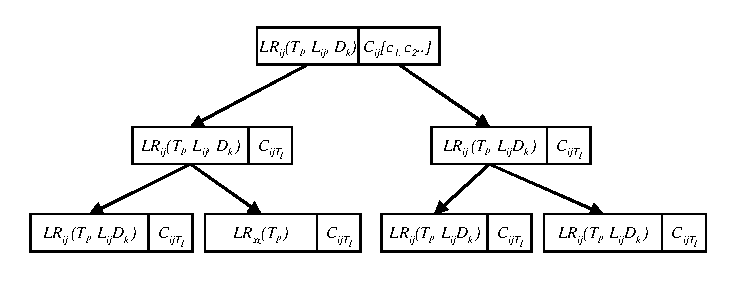
\includegraphics{Figures/LRT.eps}
\caption{Hierarchical link resource tree organization}
\label{fig:LRT}
\end{figure}

\section{Proposed Link Resource Tree Aggregation}
In this section, we propose extensions to Shared Risk Link Groups (SRLGs) tree representation technique [NAS04] that permit the computation of diverse working and protecting paths with differentiated protection levels along multiple vertical and/or horizontal domains. Our scheme proposes a link resource aggregation scheme that applicable to abstract links that we refer to as Aggregate Link Resource Trees (ALRT) representation.

 this model, every link at a given layer is associated with a Link Resource Tree (\gls{LRT}) as shown in Figure~\ref{fig:LRT}. The root of the tree is the resource parameters of the link at that layer, and the leaves are the LRTs of abstract or physical links that the given link is tunneled through at lower layers. The link parameters constitute of properties pertaining to the link's QoS state as well as its protection \gls{SRLG} group at a specific switching layer.

Among other properties, the concept of \gls{LRT} generalizes the notion of link diversity to take into account multiple layer of diversity. To provide failure-diversity at a client layer, we propose an abstraction scheme for diversity at the server layer. Here, the upper layer (encompassing lower layers) is referred to as the client layer, and lower layers are referred to as the server layers. In such a topology, a link at the client layer (for example, an IP link) can mean many nodes and links in the server layer (for example, SONET/SDH, optical and fiber level).

Figure~\ref{fig:LRT} shows how a link at client layer $T_l$ $(0<T_l<8)$ can be associated with a LRT  $(LR_l(T_l, L_{ij}, D_k), C_{ij})$where $L_{ij}$ represents the link identifier and $D_k$ identifies the domain that the link belongs to, and the triplet $(T_l, L_{ij}, D_k)$ signifies the link's resource attribute at layer $T_l$. The LRT at layer $T_l$ becomes the head of a tree whose leaves are LRTs at layers below it. The above procedure essentially creates a hanging LRT from every link at each layer.

\subsection{Inherent Properties of Link Resource Trees}
Firstly, the LRT tree conveys to the client layer any topological information changes in lower layers. For example, if a link in a lower layer is taken out of service for maintenance or upgraded, links at the client layer tunneled inside that same link are also taken out of service or notified of the change in the QoS and/or bandwidth change. These links can easily be identified if information about the out-of-service link is propagated upward along the LRT tree. In addition, the below are properties of LRTs:

\begin{definition}{Multiple inheritances} a child resource can have more than one ancestor resource. In this case, for example, a failure of a given link may be caused by a failure of one of many links at the lower layers through which the given link is tunneled in.
\end{definition}

\begin{definition}{Failure propagation} the \gls{LRT} tree also conveys to the client layer the topological changes in the lower layers. If a link in a lower layer fails or is taken out of service for maintenance/upgrade, all the links in the client layer (upper layer) that are tunneled inside the server link are directly affected and are also taken out of service.
\end{definition}

\begin{definition}{Protection bandwidth propagation} A resource may carry the working paths of several connections established at any particular client layer. If the resource fails, the connections are restored (if protection is requested) by redirecting them to their backup paths in the client layer. In order to restore these connections, some amount of backup bandwidth will be required on the links along the backup paths. A failure of a child of the above resource will require at least the same amount of backup bandwidth on these links as well. Hence, when an amount of bandwidth is reserved on a link at any given layer it must also be reserved on all links at lower layers through which the link is tunneled in.
\end{definition}

\begin{definition}{QoS parameter propagation} A link typically carries quantitative performance attributes that various classes of service normally are required to meet. An example of such attributes are packet-layer specific (\eg delay, delay-jitter, packet loss-rate), or optical-layer specific (for example, optical SNR, wavelength registration, \etc). In this case, each node in the LRT carries link attribute information about at that specific layer. Based on the metric, the ancestor can be derived from children's parameters by either recursively adding (\eg for additive metric like delay), multiplying (\eg for multiplicative attributes like availability), or choosing the minimal value (\eg for convex attributes like bandwidth).
\end{definition}

\subsection{ALRT for Horizontal Partitions}
The computation of optimal and diverse paths between end nodes of different domains requires intelligent topology abstraction with the necessary SRLG information per layer being present. The applicability of the LR tree organization per link presented earlier can be extended to abstract links-defined as sequence of physical links at a certain switching layer and included in the same domain. The domain can be a group of resources (nodes and links) that provide similar capabilities and that share the same set of risk(s) (refer to Section~\ref{TopologyLinkStateAggregation}). This abstraction of SRLG resources in a domain can be useful in summarizing and reducing the amount of information propagated in the routing protocols across layers and in hiding the topology of the domain for the sake of loose path specification, and distributed diverse path calculations.

\begin{figure}
\centering
\includegraphics[clip]{Figures/ALRT1.eps}
\caption{Example of a hierarchical ALRT organization}
\label{fig:ALRT1}
\hfill
\centering
\includegraphics[clip]{Figures/ALRT2.eps}
\caption[ALRT formation]
{ALRT formation: (a) relaxed individual trees, and (b) aggregated tree}
\label{fig:ALRT2}
\end{figure}

The ALRT tree can formed between domain-gateways in each domain as follows. For each border-gateway pair in the domain, one or more paths are computed (\eg a path per class of service supported by the domain). Each path is composed of a concatenation of a number of individual links, each associated with an individual LR tree consisting of ancestor and children resources as described in previous section (see Figure~\ref{fig:LRT}) .
 
The ALR trees of the links between the gateways become supersets of all the information contained in individual LRTs along the path. Each ALR tree is defined by one SRLG type-1 head and several SRLG type-n leaves underneath. The following steps are followed for the formation of such an ALR tree:

\begin{itemize}
\item Replace all type-$1$ heads (IT at switching layer $L_1$) by one type-1 head in the ALRT.
\item If any of type-$1$ LRs in any of the ITs is connected to a type-$n$ $(n>1)$ resource, a type-$n$ resource is also connected directly to the head in the ALRT
\item Starting with the head of the formed AT, for all successors replace all individual links that share the same domain D.
\item The trees are traversed a step lower, and above steps are repeated for the type-2 resources, and so on.
\end{itemize}

\section{Application to Multi-domain WDM Networks}
The increase in demand for bandwidth from user applications has paved way for numerous innovations in Wavelength Division Multiplexing (\gls{WDM}) networks that are capable of transporting multi-gigabit signals faster and for longer distances over a single optical fiber. An all-optical wavelength-routed WDM network consists of optical wavelength routing nodes interconnected by optical fiber links. In order to transfer data, a connection-oriented optical communication channel-- typically referred to as a lightpath is usually established over a number of optical nodes or cross-connects (\gls{OXC}s).

One of the key challenges in any QoS-based network environment is that of finding QoS guaranteed paths since they form the basis for higher-level QoS dependent services. In general, the provision of certain QoS requirements between two end-points in a network depends upon the performance properties of individual network elements such as links and nodes (\eg delay, loss rate, error rate, etc.) QoS routing tries to select a feasible path that satisfies the set of required constraints, while also achieving overall network resource efficiency. It has been found that computing a path that is subject to multiple additive constraints is an \emph{NP}-complete problem with complexity of finding a solution, in the worst case, growing exponentially with the size of network.

In wavelength-routed networks, QoS-based routing affects the routing decision (\ie choice of traversed links), as well as the selection of dedicated wavelengths.

The objective of a QoS routing scheme is to select network paths with sufficient resources to satisfy a connection's QoS request. In general, the provision of certain QoS requirements between two end-points in a network depends upon the performance properties of individual network elements such as links and nodes (\eg delay, loss rate, error rate, \etc). QoS routing tries to select a feasible path that satisfies a set of required con-straints, while also achieving overall network resource efficiency. It has been found that computing a path that is subject to multiple additive constraints (e.g., delay, SNR degradation) is an $NP$-complete problem that cannot be exactly solved in polynomial time [5].
In all-optical WDM networks, the performance of a network depends not only on the available physical re-sources (e.g., OXCs, converters, fiber links, number of wavelengths per fiber, \etc), but also on how it is con-trolled. The objective of an RWA algorithm is always to maximize the number of connection requests serviced given certain user requirements and network resource constraints. Moreover, in optical networks that are architecturally heterogeneous or spread over multi-vendor do-mains, the performance of the management and surveillance functions, as well as the network policies differ for different routes and wavelengths.

In large topology networks, topology aggregation is adopted as a technique to reduce the message overhead involved in QoS routing and achieve a scalable architecture. For example, in a multi-domain internetwork like the Internet, each ABR in each domain constructs aggregate information of two parts: (a) aggregate information about connectivity and (b) aggregate information about resource availability in the domain.

For example, in Fig. 2 the intra-routing algorithm calculates an internal path or a set of paths between the two \gls{ABR}s (A) and (B) and assigns its metrics to the logical link in the topology aggregate. After constructing such an aggregate, a domain advertises it to all other ABRs.
Hence, the routers in the internetwork will have detailed information about their own domain's state and aggregated information about other domains states. Inter-domain routing decisions are based on the aggregated state information while intra-domain routing decisions are based on the detailed state information. 

Hierarchical QoS routing is the process of selecting a path based on this mixture of detailed and aggregated state information. In this model, a signaling or call-processing entity in each domain will compute intra-domain path or paths between border routers using detailed information about the domain's internal topology and advertises the logical link's attributes to neighboring domains. Based on the aggregate advertisements between domains, the source-domain call processing entity or ABR calculates a feasible ``loose route'' for the connection that satisfies the end-to-end QoS requirement.

\begin{figure}[t]
\centering
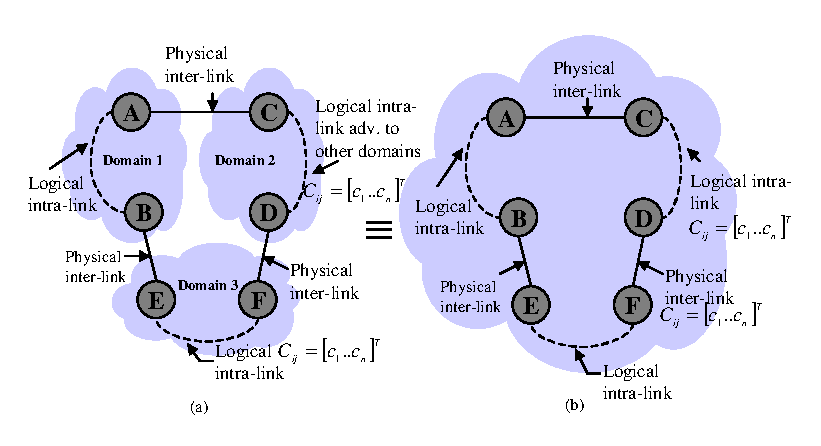
\includegraphics{Figures/MultiDomainAbstraction.eps}
\caption[Hierarchical multi-domain network]
{Hierarchical multi-domain network:
 (a) hierarchical representation,
 (b) transformed flat topology network
}
\label{fig:MultiDomainAbstraction}
\end{figure}

\subsection{Network Model}
We represent a point-to-point multi-domain communication network by a global bi-directional graph of abstract nodes $G_g(V_g, E_g)$ with $V_g$ global abstract nodes (domains) and \eg global uni-directional set of edges (inter-links) connecting different domains. Each global abstract node represents a separate domain network and is internally modeled as another directional sub-graph. $G_n(V_n, E_n)$ corresponds to domain $n$'s graph with $V_n$ set of nodes representing (optical switches) and $E_n$ set of uni-directional edges, representing to the set of intra-domain links connecting optical switches, where $n=1,2,\cdots,N$ corresponds to a domain in the global graph. We assume for every $(vi, vj)$ in $V$, there is maximally one directed edge between $v_i$ and $v_j$. Each link in the graph is characterized by a set of quality attributes parameters to reflect the quality performance on the link. To compute a cumulative feasible path, the attributes can be additive (e.g. delay, optical SNR), multiplicative (e.g. reliability) or restrictive (e.g. number of available wavelengths).

Moreover, the feasibility objective can be \emph{minimization} or \emph{maximization} of the cumulative path information. For example, ``maximum SNR path'' or ``most-reliable path'' objectives require the path with the maximum cumulative weight, while ``minimum number of hops'' or ``minimum SNR degradation'' the minimum cumulative weight [5].

\begin{figure}[t]
\centering
\includegraphics[clip]{Figures/MConstraintLink.eps}
\caption{Multi-cost abstract link translation}
\label{fig:MConstraintLink}
\end{figure}

It is known that multiplicative constraints can be transformed to additive with an additional transformation step. Also, in the case of concave (or restrictive) constraints, the problem can be further simplified by first pruning out all links that do not satisfy these constraints. Hence, in this paper we mainly focus on additive QoS parameters, namely delay and cost. Cost of the link is typically intended as an abstraction that could, in practice, be mapped into a number of link metrics (\eg available wavelength or number of calls using the link). For our simulations, we assign an adaptive cost c to each intra and inter link in our network that is dependent on  , the number of free available wavelengths on link $(v_i,v_j)$, as follows:

\begin{equation}
c_{ij} =
\begin{cases}
-log(1-\frac{1}{\lambda_{ij}^a}), &\text{$\forall \lambda_{ij}^a < 1 (i,j) \in E$} \\
1, &\text{otherwise}
\end{cases}
\end{equation}

Here, the term $(1-\frac{1}{\lambda_{ij}^a})$ denotes the measure of willingness a link offers to accept a call request. The greater the number of available wavelengths, the lower is the probability that a request will be blocked. Given a graph $G(V, E)$ and a source node $s$, a destination node $t$, and a constraint vector $c = [c1, c2, \dots, c_k],  (k \ge 2)$, we denote by $p$ a path from $s$ to $t$ as a multi-constrained path (MCP) if $w_l(p) \leq c_l$ for any $1 \leq l \leq k$. For short, we write $w(p) \leq c$. Note: $w(e)$ and $c$ are both $k$-dimensional vectors.

For a given QoS request and its constraint vector $c$, QoS routing seeks to find a feasible path $p$ satisfying $w(p) \leq c$ based on the current network state information.

By proposing energy functions, multiple QoS weights can be translated into a single metric. For example, to simplify the 2-constrained QoS routing problem, Jaffe [XXX] proposed heuristics based on the convergence of multiple weights. He proposed the linear energy function $g(p) = a_1w_1(p)+ a_2w_2(p)$, where $wi(p)$ is the $i$'th weight of path $p$. He concluded that for a given constraint vector $(c1, c2)$ of a QoS request, when the path $p$, found by Dijkstra's algorithm by minimizing $w(p)$, is feasible with maximum probability [1].

One of the problems studied in this class of con-strained-based path problems is the least-cost delay con-strained routing problem [6]. Delay constraint is a very common requirement of many multimedia and realtime applications. Cost minimization captures the need to dis-tribute the network resources efficiently amongst the various calls.

In our simulations, we restrict our study to the 2-constraint problem (\emph{cost} and \emph{delay}). We also adopt the earlier mentioned heuristic approach by Jaffe to solve for the multi-constraint shortest path problem. Hence, path $P = (v0, v1, v2, \cdots vn)$ has two associated characteristics: 

\begin{eqnarray}
Cost \qquad C(P)=\sum_{i=0}^{n-1}C(v_i,v_{i+1}) \\
Delay \qquad D(P)=\sum_{i=0}^{n-1}C(v_i,v_{i+1})
\end{eqnarray}

In Figure~\ref{fig:ExpResults-01}, we show a sample hierarchical network of interconnected domains, and the equivalent transformed graph of interconnected border routers.

\subsection{Experimental Results}
We present a study that addressed the mentioned problem of dynamically provisioning an end-to-end paths at the optical layer subject to user and network constraints and spanning multiple wavelength-routed WDM optical domains. A hierarchical connection-provisioning algorithm for the computation and setup of the end-to-end constraint-based path was proposed.

In this section, we present experimental results of simulations run on a 40-node, 72 bi-directional links, and 4-domain meshed network. All links in the network are assumed to have a 4-wavelength capacity. 
Each node in the network is defined by a tuple $(node_id, domain_id)$. Call requests in each domain are generated according to a \emph{Poisson} process with an arrival rate $\lambda_i$. The holding time for a call is exponentially distributed with an average mean $\mu_i$. The traffic load per domain is obtained by the formula $i =\lambda_i \dot \mu_i$. The source-destination pair $(s, t)$ for each call is selected randomly with a uniform probability for local and global traffic.

We assign link delays to normalized uniformly distributed random numbers. For each QoS request, we randomly generate the 2-constraints delay,  and cost with uniform distribution. In our simulations, we also assume that call requests are equally probable to be local and global. For the allocation of an available wavelength, we apply the First-Fit (FF) wavelength assignment algorithm.

In each experiment we generate 100,000 call requests and measure the blocking probability of the network. Blocking probability is defined by the ratio of number of blocked calls to the total number of calls generated.

\begin{figure}[t]
\centering
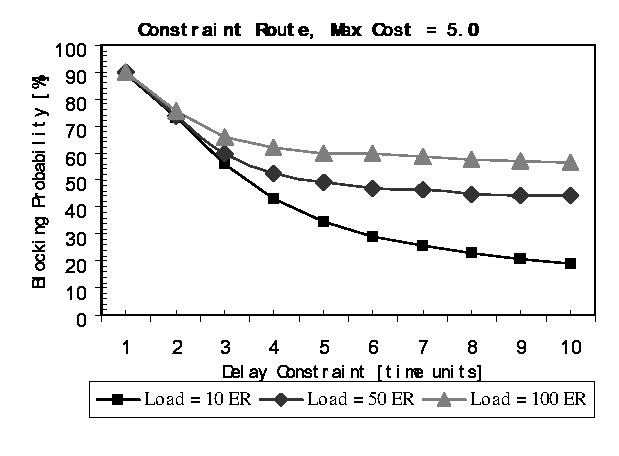
\includegraphics{Figures/InterdomainWDM.eps}
\caption[LSP blocking probability]
{LSP Blocking probability versus delay constraint for different aggregate traffic load per domain}
\label{fig:InterdomainWDM}
\end{figure}

In Figure~\ref{fig:InterdomainWDM}, we show the blocking probability of the QoS call requests versus the maximum delay constraint. It is clear that the blocking in call requests decreases as the dominating constraint of QoS calls is relaxed (i.e. delay  ). Also, as the traffic load per domain increases, more QoS call requests are likely to be blocked resulting in higher blocking probability.


\section{Conclusions}
In this chapter, we presented an aggregation of topology and network state information is implemented to achieve control layer scalability as well as reduce the complexity of the path selection algorithms. To achieve this, an efficient aggregation scheme is needed to convey the necessary information (e.g. bandwidth state, QoS, or protection SRLGs), reduce the frequency of crank-backs happening at signaling time, and achieve faster setup times for connections. For this, we propose a novel link aggregation scheme that is capable of addressing the former challenges. In the course of completing this thesis, we will expand on our study of the performance of implementing such a scheme in a multilayered multi-domain networks to reduce the connection blocking ratio, the frequency of crank-backs, as well as LSP setup time.

In the inter-carrier inter-domain case, we studied the challenges posed in signaling an end-to-end service guaranteed LSP in the presence of minimal or no exchange of network state information between adjacent domains. To address this problem, we propose to employ 2 potential solutions: 1) a game theory approach to optimize the coordination and partitioning of the overall service among all transiting domains, and 2) a discovery message flooding mechanism to collect the service constraint on per domain for each of the transit domains and allow the receiver to make the most favorable decision on path selection. We anticipate the conclusion of this thesis will provide ample analysis and performance evaluations for the above two proposals.

\chapter{Service Guaranteed Inter-AS Traffic Engineering}
\label{chap:ServiceGuarTE}
\markright{Service Guaranteed Inter-AS Traffic Engineering}

\section{Background}
Today's Internet is composed of approximately 20,000 competing autonomous systems (ASes) which have to cooperate with each other to provide the end-to-end services across them. Each AS is typically controlled by a different administrative entity, and therefore encodes various economic, business, and performance decisions in its routing and TE policies. Due to security concerns, when different carriers administer networks, they will not disclose any sensitive internal information about their network topology to neighboring carriers (who may be competitors). For example, carriers may be reluctant to disclose details of the bandwidth available within their network or whether their topology allows them to protect a particular LSP. This makes it much harder to design an efficient path computation algorithm that can calculate routes spanning multiple carriers.

The advent of distributed control plane technologies such as MPLS and GMPLS has opened the door to an array of end-to-end QoS-based services that were previously hard to provide over the shared Internet. The global adoption of service delivery using these technologies assumes that users can be provided connections with well-defined attributes that will not change over the service delivery period with changes in network or user population. Fundamental to this assumption is the ability to dynamically compute routes through the network that satisfy certain connection attributes (\eg\ administrative or other types of constraints). In this context, constrained-based routing or path-computation is an essential functionality in MPLS, GMPLS, or any control plane architecture with end-to-end performance objective.

In Chapter~\ref{cha:PathCompTechniques}, we presented a number of techniques for computing inter-domain paths. Among these, the PCE scheme is well suited for computing paths that span multiple ASes. However, this scheme assumes either a priori knowledge of the AS path the inter-AS LSP will take, or the dynamic selection of next-hop PCE (\eg based on preferred BGP next-hop). As a result, the existing proposals still fall short from finding an optimal inter-AS feasible constrained path. 

In this Chapter, we present a novel PCE-based scheme that we propose as a solution for the inadequacies of existing mechanisms. We investigate the problem of handling end-to-end constraints across multiple service provider networks without requiring any internal network information which is usually the case in inter-carrier multi-domain connection setup scenarios. We assume the users specify, on a per-connection basis, absolute parameter bounds such as the maximum bandwidth, maximum delay, and minimum connection availability. Typically network providers offer a a variety of different services at different prices.

\section{Problem definition}
There are two requirements that carriers are continuously striving to find novel solutions for :
\begin{itemize}
\item \textbf{reliability}-- for example, in order to meet end-user requirements for service availability, traffic may need to be protected by a diverse backup connections
\item \textbf{quality}-- in accordance with SLA that is contracted with  customers, and the type of data transported (for example, minimal and consistent delay for voice traffic).
\end{itemize}

Furthermore, carriers require that, wherever possible, data be transmitted following a path which minimizes the impact on the performance of the carrier's overall network. Today most carriers are deploying MPLS and GMPLS in their networks to ensure that the above requirements can be met. However, in order to set up TE LSPs that satisfy certain that meet these requirements in terms of quality and reliability, carriers must be able to compute and reserve resources over a suitable path (or sequence of sub-paths) across their network(s).

For the intra-domain case, there are well understood methodologies for selecting such a TE path. In this case, the TE topology and related TE link attributes (\eg\ QoS, and/or resource availability) are flooded using extensions to existing routing IGP protocols such as OSPF and ISIS. Every LSR within an IGP domain or area has visibility over the full TE topology and is able to run a CSPF algorithm to compute an end-to-end constrained path for an LSP.
However, extending this service across different areas or ASes becomes not trivial. In this case, the desire of SPs to hide their internal topology and the need to compute constrained LSP paths are not easily simultaneously satisfiable. In a hierarchical network, different routing protocols can be used at different levels of the network.

The most prominent Internet inter-domain routing protocol today is the Border Gateway Protocol (BGP). BGP is a path vector based protocol, where a path refers to a sequence of intermediate domains between source and destination routers. BGP only provides reachability information for the destinations. More precisely, it only provides the addresses of Next Hops (NHs), the nodes at the border of the domain, that are able to forward the packets to a given destination. The QoS properties of the paths, such as the delay and bandwidth, behind these NHs are not provided. This results in several limitations for the computation and establishment of constrained interdomain LSPs.

While the existing path computation techniques that we have mentioned in Chapter~\ref{cha:PathCompTechniques}  may be sufficient for some inter-provider deployment scenarios, it may be desirable to select among multiple available inter-domain paths based on the QoS and cost requirements for different classes of traffic. That is, there may be cases in which the current path selection capabilities of BGP, which yield only a single best path for a given prefix, may not yield a feasible path that satisfies the end-to-end service requirements for a connection.

Also, since every domain is allowed to use its own policy to determine routes, the final outcome may be a path that is locally optimal at within some domains but globally sub-optimal due to the lack of a uniform policy or metric used to find an end-to-end route.

\section{Service Level Agreements}
A Service Level Agreement (SLA) is a contract in which a certain level of service is agreed between a service provider and a service consumer. It may specify the levels of availability, serviceability, performance and operation conditions.
In a multi-domain environment where applications or users require resources from different service providers the issue of acquiring a specified level of QoS is of great importance.

Different network providers offer a variety of differing services at different prices. A Service Level Agreement (SLA) between the Service Provider (SP) and its customer usually defines the level of the service that is agreed upon between them. It typically specifies levels of availability, serviceability, performance and operation conditions. SLAs are attractive to service providers since they permit differential treatment and provide incentives for users to choose the service that is most appropriate to their needs, thereby discouraging over-allocation of resources and maximizing statistical multiplexing capabilities. To customers, on the other hand, SLAs can play be decdefine measurable levels of the service performance they expect and pay for, and in turn, a way to demand for compensation for the lack thereof.

Given the large number of inter-connected networks in the Internet, it is likely that a LSP connection originating in one SP will traverse multiple ISP networks before reaching its destination. Moreover, it is possible that multiple ISPs can collaborate to provide the requested end-to-end service. To guarantee certain QoS assurances to the end-to-end path, the complete path should be configured and reserved to offer the particular requested service and the global network setup should be compliant and aware of the service being offered. By offering end-to-end SLAs, ISPs could collectively profit from higher revenue traffic. At the same time, a customer whose sites belong to different ISP networks could benefit from the same kind of performance assurance a single-ISP customer receives.

\section{Service Availability as a Path Constraint}
Assuming that an inter-domain LSP path $p$ traverses domains $D_1, D_2, \ldots, D_n$. Then, path $p$ is a reliable path for connection $t$ only if it satisfies the inequality:

\begin{equation}
\label{eqn.availabilityProduct}
 Ap = \prod_{i=0}^{n}\left({A_1\times A_2 \times \ldots \times A_n}\right) \geq A_t
\end{equation}
where Ai is the availability of the selected service j in domain i, and A't is availability requirement of connection t. Computing the logarithm and multiplying both sides by -1, while noting that service availabilities are between 0 and 1, we get:
\begin{equation}
-log(A_p) = -log(A_1) - log(A_2) - \ldots - log(A_n) \leq -logA_t
\end{equation}

Now, if the cost of link $L_i$ $(C_i)$ is defined as a function of its availability (i.e., $Ci = -log(A_i)$, the cost is additive and the path with minimum cost will be the path with maximum availability (such a path is called the most reliable path (MRP)). This Multiplication-to-Summation (MS) technique can be used to compute the MRP. If the availability of a MRP is lower than $A_t$, then the path is not reliable enough for connection $t$. Note, in this case the availability of a sub-path or link can be increased as mentioned in Chapter~\ref{eqn.availabilityProduct}. 

Cooperative PCEs


\chapter{Evaluation of PCE Selection Schemes}
\label{chap:EvaluationPCESelectionSchemes}
\markright{Evaluation of PCE Selection Schemes}
%======================================================================
\section{Background}
%======================================================================

\section{PCE Architecture}
The notion of Path Computation Element (PCE), originally named Path Computation Server (PCS), was initially introduced in order to solve the specific issue of inter-domain path computation for TE LSPs. The basic idea was to rely on the collaboration of ABRs or ASBRs to compute a TE LSP spanning multiple IGP areas or ASes.
The PCE framework [88] provides functions and protocol-extensions to address the computation of paths spanning multiple TE routing areas or administrative domains. There are several motivations for PCE-based architecture; among those are offloading the highly CPU-intensive path computation functions from control plane of core routers to some other devoted network routers or PCE(s).
Using the PCE architecture, prior to signaling an LSP that spans multiple domains, the TE LSP path is computed distributively and collaboratively� optionally applying various computational constraints� through communicating between cooperating PCEs usually residing at domain borders or exit points. Of particular interest in this chapter, is cooperative nature of PCE path computation. We show that depending on the information available to each PCE it is possible to enhance the total path computation time for the inter-domain LSP path, and consequently improve the blocking probability of the LSP.

The PCE is usually used as a generic term to define the overall architecture (specified in [88]), which is made of several components:
Traffic Engineering Label Switched Path (TE LSP): a unidirectional MPLS connection whose path is determined under certain QoS constraints by a TE module and defined as a collection of strict and/or loose hops.
The Path Computation Client (PCC): an entity originating a path computation request to a PCE (Path Computation Element) to compute a TE LSP. The PCC is typically an MPLS LSR (Label Switching Router).
The Path Computation Element (PCE): an entity (component, application or network node) that is capable of computing a network path or route based on a network graph and applying computational constraints.
PCE Protocol Signaling (PCEP): a PCC or PCE communicates with other PCE using a defined signaling protocol called PCEP and specified in [90].
PCE discovery: PCC(s) or PCE(s) can either use statically defined set of PCE(s) to consult for the path computation or discover the presence of PCEs and their capabilities using some discovery protocol (e.g. using extension to existing IGP flooding protocols like OSPF and ISIS).
Path Computation procedure: there are several PCE path computation techniques presented in the literature. Among those is the Backward Path Recursive Computation defined in [89]. As pointed out, the PCE can be used to cope with complex path computation problems in the context of intra-domain, inter-domain with partial domain visibility (case of inter-area or inter-Autonomous System (AS), or packet/non-packet domain in the context of GMPLS). In this document, we focus on the inter-domain MPLS TE case with BRPC.
PCE Policy: when PCE-based computation procedures are used to compute inter-AS TE LSP spanning multiple ASs managed by different Service Providers, policy becomes a key component of the architecture responsible for ensuring that path computation requests are directed to a specific PCE according to pre-established contract agreement (rate at which requests are sent, total amount of requested bandwidth, total number of TE LSPs, accounting, etc�). Furthermore, in some case, crossing AS boundaries require constraints mapping (bandwidth pool, preemption, affinity, etc�) should the two neighboring ASs make use of different conventions.
Traffic Engineering Database (TED): contains the topology and TE link resource information of the domain or area usually populated using extensions to IGP protocols like OSPF or ISIS, or other means (e.g. by a management application).

\subsection{PCE Path Computation Procedure}
One or more PCE routers typically residing at the domain or area borders are capable of performing optimal and/or diverse TE path computation for TE LSPs on behalf of other domain nodes usually referred to as PCCs. In the context of multi-layer networks, a PCE typically resides at the border of the adjacent layers (e.g. packet, optical, etc.) and accepts requests for hierarchical TE LSPs from the client upper layer (e.g. packet layer) and supplies the end-to-end multi-layer path.
When using PCE, the path computation for the TE LSP does not occur at the head-end (ingress) of the TE LSP. Instead, the head-end acting as a PCC determines and forwards the request with the desired path computation constraints to one of eligible PCEs capable of further processing the request (see Figure 1.2). The path computation request is then relayed until reaching the PCE that can resolve the full path to the inter-domain LSP�s destination node. 
Using BRPC, once the PCE determines that it can not solely compute the end-to-end path, it can consult other PCE(s) present neighboring domain(s) to do so.
If no next PCE can be found or if the next hop PCE of choice is unavailable, the procedure stops, and a path computation error is returned.  If multiple PCEs capable of serving the computation request are discovered, the upstream PCE may select a subset of these PCEs based on some local policies or heuristics (see Figure 1.3).

When a PCE receives a request for which it has direct visibility to the TE LSP destination node in its TED, it performs a local path computation for the shortest path from an ABR to the destination node, and replies back with the path to the upstream PCE. The upstream PCE in their turn append their own local domain paths to the full path and forward the PCE reply eventually to the PCC �the initiator of the request.
In the remaining of the chapter, we will study the effect of the PCE selection scheme on the path computation time and the LSP blocking probability. We will also present two heuristics to enhance this probability.


\subsection{PCE Selection for Path Computation}
Requests for path computation of an inter-area/domain TE LSP can be performed by either using a centralized PCE instance that has TE visibility over all of the other areas/domains, or can be distributed among multiple PCE instances �one responsible for each domain. In the latter case, when a PCE is not able to compute the full end-to-end path, a decision has to be made to select and forward the computation request to a downstream PCE node. This downstream PCE node selection process is crucial in the amount of overall time taken to compute the full end-to-end path. Typically, routing information � e.g. reachability to the destination announced by area border routers or autonomous system border routers or another user set routing policy� is used to define a set of eligible PCEs that are capable of processing further the path computation request.

However, among the set of candidate PCE(s), the decision to elect a certain PCE and forward the path computation request can affect significantly the overall end-to-end path computation response time depending on the degree of congestion on this PCE and the available resources for the computation process. Consequently, as the path computation time increases significantly, the signaled LSP can be potentially blocked at transit nodes due to reasons like: 1) the PCC can timeout waiting for the expected path reply after crossing a certain acceptable time threshold, 2) due to network state dynamics in each of the traversed domain(s) due to resources no longer available (e.g. due to other competing intra/inter-area LSPs), specifically after a considerable time had elapsed from the time of last path computation in that domain.

\section{Proposed PCE selection schemes}
There are a number of schemes that can be considered to elect a preferred PCE from a set of candidates that can collaboratively compute the overall end-to-end inter-area or domain TE LSP�s path. In this section we present two approaches that attempt to forward the PCE requests to PCEs that are less loaded.
In the first approach, the selection decision is done on per PCE-hop to determine the next hop PCE to further process the path computation request. Each PCE keeps a record for the performance measure to peering PCE(s) (e.g. the path computation response time) and utilizes this in its decision making. We refer to this approach as per-Hop PCE selection.
The second approach relies on keeping an average of the response time for each downstream PCE and sharing this state with a tier-1 PCE instance that overlooks over all other areas. We refer to this as source-specified PCE approach (SSPCE).
We describe in more details the 2 approaches and present some results for simulation runs that we collected on the topology described in Figure 1.9.

\subsection{Analysis and Mathmatical Model}
We assume that each PCE can be modeled as an $M/M/1$ queue where path computation requests arrive at rate $\lambda_p$. Each PCE takes, on average, time $T_p$ to process a request with the average path computation serviced rate $\mu=\frac{1}{T_p}$. The expected response time at $PCE_p$ can be written as:

\begin{equation}
E(t)=\dfrac{1}{\mu_p-\lambda_T^p}
\end{equation}

and  $\lambda_T^p$ being the total rate of arrival of path computation requests from all possible upstream PCE(s) to node $p$.

\begin{equation}
\lambda_T^p=\sum_{i=1}^n\lambda_i^p
\end{equation}

The expected number of requests R queued in PCE p can be written as:
\begin{equation}
E(R)=\dfrac{\lambda_T^p}{\mu_p-\lambda_T^p}
\end{equation}

Considering the case where arriving requests at a PCE node can be forwarded to $m$ downstream PCEs. The probability that any particular PCE request is directed to a particular PCE is $\frac{1}{m}$. It follows the probability that exactly $x$ out of $R$ requests are directed to that PCE is:

\begin{equation}
P(x)=
\begin{pmatrix}
R  \\ 
x  
\end{pmatrix}
m^{-R} (m-1)^{R-x}
\end{equation}

where,
\begin{equation}
\begin{pmatrix}
R  \\ 
x  
\end{pmatrix} = \dfrac{R!}{x!(R-x)!}
\end{equation}

The following properties then apply:
\begin{enumerate}
\item The stability condition is given by $\lambda_T \langle m\mu$.
\item The quantity $\rho=\frac{\lambda_T}{m\mu}$  gives the utilization of a single server.
\item The steady-state probabilities for $\rho \langle 1$ are given by:

\begin{equation}
p_0= \left[ \sum_{k=0}^{m-1} \dfrac{(m\rho)^k}{k!} +
\left( \dfrac{(m\rho)^m}{m!}\right) 
\left( \dfrac{1}{1-\rho}\right) 
 \right]^{-1}
\end{equation}

\begin{equation}
p_k= \begin{cases} 
p_0 \dfrac{(m\rho)^k}{k!}, & k\leq m \\
p_0 \dfrac{m^m\rho^k}{m!}, & k \geq m
\end{cases}
\end{equation}

\end{enumerate}

For example, consider the case where a PCE takes on average $T=2.5\,milliseconds$ to complete a TE path computation transaction, (i.e. requests are serviced at rate $\mu=400\,req/sec$), Figure XXX shows the expected number of PCE requests queued as a function of load utilization $\rho$. As the total rate arrival of PCE requests ?T approaches the rate of service the path computation requests $\mu$, the number of queued PCE requests and subsequently the expected response time increases significantly.

Within a time period $t_x$, assuming $x$ requests arrive at a certain PCE $p$, as long as $xT < t_x$ there will be no queuing of requests at PCE $p$; the latency experienced in this case for each request will be $T$, usually negligible. When $xT > t_x$, the request processing rate is limited by the server, each request averaging one transaction in each period $xT$. The extra delay per each request transaction is $(xT - t_x)$.

We can observe from previous discussion that the number of redundant/eligible PCEs m that can process a certain path computation request plays a key role in bounding the maximum response time experienced by the request. In general, the base (minimum adequate) number of PCEs must provide acceptable response time, so must not be very far into the overload region.

\subsubsection{Source Specified PCE Selection}
This scheme assumes that each PCE keeps track of mean aggregate arrival rate of path computation requests and uses this information to periodically flood a metric associated with the cost of using that PCE for a path computation. Each PCE creates a PCE virtual topology in the form of a graph $G(V,E)$ where $V$ corresponds to the set of PCEs in all areas, and $E$ the set of virtual links/edges between peering PCEs and whose link-weights reflect the amount of system utilization for that downstream PCE (see Figure 1.7). In summary, PCEs that are highly utilized will flood a large metric to be used for the virtual links and consequently will be avoided in any future path computations.

The originator of the PCE request (e.g. PCC or PCE) directs the PCE request to a PCE in its domain. In turn, the PCE computes the least PCE utilized path that is capable of computing the end-to-end inter-area path. The PCE-hops sequence can then be carried in the PCEP path computation request message and be used at each PCE hop to forward the requests downstream

In order to define a meaningful link cost associated with expected response time when using that PCE, we attempt to model each PCE as an $M/M/1$ queue. 
Equation 5.7 defines the PCE utilization $(\rho_p)$ which represents the amount of load at any PCE router $p$. It is defined as the ratio of the total request arrival rate $\lambda_T^p$ to the request service $rate \mu_p$:

\begin{equation}
\rho_p = \dfrac{\lambda_T^p}{\mu_p}
\end{equation}

The load intensity on each PCE which serves as an indication of the total number of requests queued awaiting processing at PCE $p$ is shown in Equation 1.9.  Note as $\rho\longrightarrow1$, the cost the virtual link to use PCE $p$ increases dramatically. This means that as the PCE server queue grows in size the PCE is penalized by increasing this cost so that incoming requests can use other PCEs to compute their path.

\begin{equation}
c_p=\dfrac{\rho_p}{1-\rho_p}
\end{equation}

\section{Per-hop PCE Selection}
This approach assumes the PCE selection is performed at each traversed PCE hop to elect a preferred next hop PCE to further process the request. Along this vein we present three methods to partition the requests: 1) by equal partitioning (e.g. round-robin distribution), 2) by forwarding requests to the PCE with least response time, and 3) using an adaptive approach to partition the requests using token quotas defined based on an average response time for each peering PCE.

\subsection{Round-robin PCE selection}
The Round-robin PCE seclection (RRS) method assumes that requests are distributed equally in a round-robin fashion among a number of eligible PCEs that are capable of processing further the path computation request. In this scheme, requests from a certain source can be assumed to be locally distributed evenly among the available candidate PCEs. However, this does not guarantee global request balancing among the all candidate PCEs, and hence, can lead to some PCEs being overloaded with large queue of requests leading to increased delays in the overall path computation response.

\subsection{Least response PCE selection}
The Least Response PCE (LRS) selection heuristic assumes that each PCE preserves locally an average path computation response time to each peering PCE. The downstream PCE would be always picked based on the least PCE response time. This scheme will achieve relatively better load request load balancing among PCEs. However, depending on the accuracy of the average response time stored locally, might not always yield the best PCE to forward to.

\subsection{Token-based PCE selection}
The Token-based PCE (TBS) selection heuristic also assumes an average response time is kept to each of the peering PCE(s). Arriving requests are partitioned among the eligible PCEs based on a token-based quota policy that is define based on the recorded average response times for each peering PCE. The main idea behind this heuristic is to penalize the PCE with the higher path computation response time by sending to it less path computation requests at any one time. Note, we assume in this case that the partitioning quotas (tokens) can be updated periodically or once every time a path computation reply is received from downstream PCE. Algorithm 1 shows the steps included in executing this algorithm.

\begin{algorithm}
\caption{Token-based PCE selection heuristic}  % give the algorithm a caption
\label{alg.TBS}
\begin{algorithmic}                    % enter the algorithmic environment
\WHILE{More PCE path compute request in queue}
\STATE Initialize token vector $T$ for all peering PCEs:
\STATE $T \Leftarrow \phi$
\STATE Find $S_r$ set of eligible PCEs for request $R$
\STATE Extract PCE $p$ with highest request tokens
\STATE Forward path compute request to $p$
\STATE Decrement PCE request tokens for PCE $p$
\ENDWHILE
\end{algorithmic}
\end{algorithm}


\chapter{Multi-layer Simulator}
\label{cha:Simulator}
\markright{Multi-layer Simulator}

\section{Introduction}
We designed and implemented a simulation toolkit to investigate path computation and performance issues in hierarchical networks. The simulator is a high level implementation of the RSVP-TE signalling protocol for GMPLS-TE networks, The C++ software has a modular architecture, allowing users to readily ``plug-in'' new code and quantitatively assess the impact of different proposed strategies on network performance. 

\section{The Model}
Connection requests are modeled by a Poission process, and connection holding time is exponentially distributed. The inter-arrival time for connection requests are exponentially distributed with a mean $\lambda$.
In order to be able to use crankback frequency as a measure of network performance, we assume that connection requests are not persistent. In other words, if a connection fails to reach its destination in-spite of all crankbacks, it does not re-initiate another attempt. 

\section {Link attributes}

To this end, we define the load being placed on the network as the product of the average request rate and average connection holding time, 
\section{Horizontal Inter-domain Simulation}
Each domain has nodes/links.

\section{Vertical Inter-layer Simulation}
Each upper layer node layer is modelled by a single domain ABR node which is connected to an ABR node at the lower-layer. It is also possible for an other non-ABR nodes to exist at a certain layer (example of those nodes are those that are directly connecting by point-to-point fibers that do not use the virtual lower layer meshed network). In lower layer, nodes (e.g. connected by fibers) can exist.
 
\section{Conclusions}

\chapter{Conclusions and Future Research}
% new right header
\markright{Conclusions and Future Research}

\section{Concluding Remarks}
We conclude this thesis proposal with a review of the addressed problems and the proposed solutions, as well as the tools that will be used to solve them. We highlight the work that has been completed and what still needs to be done to conclude the remaining part:

\begin{itemize}

\item Review of the design and planning of horizontally and vertically layered transport networks�we have conducted a broad study on how multiple switching layer interaction impacts the network design and planning, and its effect on the dynamic LSP provisioning paradigms (e,g, independent single-layer provisioning, or integrated multi-layer provisioning). We considered the challenges posed in providing the appropriate level of protection � at each individual layer� for a connection according to a predefined service availability requirement.

\item Novel hierarchical aggregation scheme� we proposed a scheme that is suitable for the integration in the border model multilayered multi-domain network architecture. The scheme defines the notion of link resource trees that encode useful information about links at each of the network switching layers (e.g. SRLG, and layer-specific QoS information). The aggregated scheme is extended to carry summarized information about abstract links between domain border nodes.

\item Intra-carrier inter-domain hierarchical QoS path calculation/selection policy� we presented a path selection scheme suitable for deployment in a multilayered transport network that makes use of the hierarchical aggregation scheme mentioned above. The scheme is capable of the computation of optimal service guaranteed and/or failure diverse LSPs across multiple switching layers and domains.

\item Inter-carrier inter-domain QoS path calculation/selection policy� we addressed an important and timely issue in today�s multi-provider networks to provide multi-carrier service guaranteed SLAs across heterogeneous networks in the presence of minimal or no exchange of network state information. To solve this problem, we propose 2 potential resolutions: 1) a game theory approach to optimize the coordination and partitioning of the overall service among all transiting domains especially when ISPs exercise heterogeneous service-cost models, and 2) a discovery message flooding mechanism to collect the service pledge on per domain for each of the transit domains. The receiver in turn, makes the most favorable decision on path selection.

\item Inter-layer coordination protection schemes� we reviewed several techniques for the coordination of the restoration procedures at different switching layers, including recovery at the highest layer, lowest layer, or timer and/or token coordinated. In our study, we will attempt to realize a suitable technique that provides efficient cross-layer and cross domain coordination for end-to-end recovery.

\end{itemize}

\section{Future Research}

This is the future research...


% Appendices
\appendix
% Designate with \appendix declaration which just changes numbering style 
% from here on
% \include{useful_pkgs} %"Some Useful \LaTeX2e Packages"
% An appendix
%======================================================================
\chapter{Sources of Information and Help}
\markright{Sources of Information and Help}
%======================================================================
The best source of information about \LaTeX\ is the two books mentioned in this course \cite{lamport.book,goossens.book}.
Another excellent resource is the UseNet newsgroup \verb=comp.text.tex=.
A frequently-asked-questions (FAQ) list is also maintained by this news group.
You might also search the World Wide Web for ``LaTeX'' for other sources of help.
 %"Sources of Information and Help"

% Bibliography 
% If done using the BibTeX program, use
% \bibliographystyle{plain} % sorted alphabetically, labeled with numbers

\bibliographystyle{alpha}  % sorted alphabetically, labeled with NAME(YEAR)% 
%%% \bibliographystyle{wmaainf}
\bibliography{bibliography/keylatex} % names file keylatex.bib as my bibliography file
\printindex

%----------------------------------------------------------------------
\end{document}
%======================================================================
